\documentclass{ctexrep}
\usepackage[colorlinks=true,linkcolor=mydarkblue]{hyperref}
\usepackage[top=1in,bottom=1in]{geometry}
\usepackage[dvipsnames]{xcolor}
\usepackage{adjustbox}
\usepackage{tcolorbox}
\usepackage{mathtools}
\usepackage{extarrows}
\usepackage{arydshln}
\usepackage{graphicx}
\usepackage{varwidth}
\usepackage{mathrsfs}
\usepackage{amsfonts}
\usepackage{amsmath}
\usepackage{amssymb}
\usepackage{amsthm}
\usepackage{braket}
\usepackage{tikz}
\usepackage{bm}
\tcbuselibrary{breakable}
\tcbuselibrary{skins}
\usetikzlibrary{
  decorations.pathreplacing,
  cd,
  arrows,
  angles,
  quotes,
  calc,
  calligraphy,
  chains,
  decorations.pathmorphing,
  intersections,
  positioning,
  shapes}

\title{数学分析 (3)}

\graphicspath{{./image/}}
\newcommand{\img}[2]{\begin{center}\includegraphics[width=#1\textwidth]{#2}\end{center}}

\newcommand{\makecolorbox}[3]{
    \newcounter{#1}
    \numberwithin{#1}{section}
    \NewTColorBox{#1box}{o m +o}{
    enhanced,colframe=#2!5!white,interior empty,
    coltitle=white,fonttitle=\bfseries,colbacktitle=#2,
    extras broken={frame empty,interior empty},
    borderline={0.5mm}{0mm}{#2},
    breakable=true,
    top=4mm,
    before skip=3.5mm,
    attach boxed title to top left={yshift=-3mm,xshift=5mm},
    boxed title style={boxrule=0pt,sharp corners=all},varwidth boxed title,
    IfNoValueTF={##1}{title=##2~\csname the#1\endcsname}{title=##2~\csname the#1\endcsname~(##1)},
    IfNoValueTF={##3}{}{##3}
    }
    \NewDocumentEnvironment{#1}{o +d""}{
    \refstepcounter{#1}
    \begin{#1box}[##1]{#3}[##2]
    }{\end{#1box}}
}

\definecolor{mygreen}{HTML}{00A652}
\definecolor{myorange}{HTML}{FF8618}
\definecolor{myblue}{HTML}{00AEF7}
\makecolorbox{definition}{mygreen}{定义}
\makecolorbox{property}{myblue}{性质}
\makecolorbox{theorem}{myorange}{定理}
\makecolorbox{lemma}{myorange}{引理}
\makecolorbox{inference}{myorange}{推论}

\newtheoremstyle{examplestyle}
  {}{}{}{}{\bfseries}{.}{0.5em}
  {\color{mygreen}\thmname{#1}\thmnumber{#2}\thmnote{#3}}
\theoremstyle{examplestyle}
\newtheorem{example}{例}
\counterwithin*{example}{subsection}

\newtheoremstyle{hintstyle}
  {}{}{}{}{\bfseries}{.}{0.5em}
  {\color{myorange}\thmname{#1}\thmnumber{#2}\thmnote{#3}}
\theoremstyle{hintstyle}
\newtheorem{hint}{注}
\counterwithin*{hint}{subsection}

\renewcommand{\proofname}{\color{myorange}\textrm{证明}}

\definecolor{mydarkblue}{HTML}{3C71B7}
\newcommand{\mychapter}[1]{{\color{mydarkblue}\chapter{#1}}}
\newcommand{\mysection}[1]{{\color{mydarkblue}\section{#1}}}
\newcommand{\mysubsection}[1]{{\color{mydarkblue}\subsection{#1}}}
\newcommand{\mysubsubsection}[1]{{\color{mydarkblue}\subsubsection{#1}}}

\newcommand{\RR}{\mathbb{R}}
\newcommand{\abs}[1]{\left\lvert{#1}\right\rvert}
\newcommand{\eps}{\varepsilon}
\newcommand{\td}{\widetilde}
\newcommand{\dd}{\mathrm{d}}
\newcommand{\pard}[2]{\frac{\partial{#1}}{\partial{#2}}}
\newcommand{\inner}[1]{\left\langle{#1}\right\rangle}
\newcommand{\grad}{\mathrm{grad}\;}
\newcommand{\curl}{\mathrm{curl}\;}
\newcommand{\ddiv}{\mathrm{div}\;}

\begin{document}
\maketitle
\tableofcontents

\setcounter{chapter}{11}
\mychapter{$n$ 维空间中的曲面和微分形式}

本章进一步研究曲面的概念,并为下一章曲线曲面积分作必要的准备。为此我们将讲述曲面的其它定义;曲面的定向;带边曲面及其定向;曲面的面积以及微分形式这些内容.

\mysection{$\RR^n$ 中的曲面}

在第八章,我们已经定义了 $\RR^n$ 中的光滑曲面. 本章我们进一步来定义一般的曲面(可能不光滑).

\begin{definition}\label{df:surface}
设 $S\subseteq\RR^n$ 非空. 设 $k\le n$.

称 $S$ 是一个 $k$ 维曲面,若 $\forall x\in S$ ,存在 $x$ 在 $S$ 中的邻域 $U$ 以及同胚映射 $\varphi:\RR^k\to U$.
\end{definition}

\img{0.5}{12.1.1.png}

直观来讲:若 $S$ 的每个局部看起来都像是 $\RR^k$ 的一个“形变”,则 $S$ 是一个 $k$ 维曲面.

\begin{definition}
上一定义中出现的同胚 $\varphi$ 称为是 $S$ 的一个图或者局部图,其中 $\RR^k$ 称为参数域,而 $U$ 称为是 $\varphi$ 的有效域.
\end{definition}

设 $S\subset\RR^n$ 是一个 $k$ 维曲面.

则对 $\forall x\in S,\exists U_x$ 以及 $\varphi_x:\RR^k\to U_x$ 使得 $\varphi_x$ 为同胚.

特别地,
$$
S=\bigcup_{x\in S}U_x
$$

事实上,可以证明:

\begin{property}
设 $S\subset\RR^n$ 为一个 $k$ 维曲面,则存在至多可数的指标集 $I$ 满足 $\forall i\in I,\exists U_i\subset S$ 以及映射 $\varphi_i:\RR^k\to U_i$ 为同胚,且有
$$
S=\bigcup_{i\in I}U_i
$$
\end{property}

即可以用可数个图的有效域覆盖曲面 $S$.

\begin{definition}
设 $S$ 是一个 $k$ 维曲面. 设 $I,\varphi_i,U_i$ 满足如上性质.

则称 $\set{\varphi_i:\RR^k\to U_i|i\in I}$ 是曲面 $S$ 的一个图册.

特别地,若可取指标集 $I$ 为单点集,则称 $S$ 是一个初等曲面.
\end{definition}

以下给出几个注记.

\begin{hint}
\begin{enumerate}
    \item 可以将曲面定义中的 $\RR^k$ 替换成任何与 $\RR^k$ 同胚的集合,例如
$$
I^k=[-1,1]^k\qquad\text{或}\qquad B^k=\set{x\in\RR^k:\abs{x}<1}
$$
    在实际应用中,我们经常取 $I^k$.

    \item 可以认为 $\varphi$ 在 $S$ 的局部引入了一个曲线坐标:对任意的点 $x=\varphi(t)\in U$ 我们给定一个坐标 $t$.

    \item 这里我们对图 $\varphi$ 仅假定连续性,从而实际得到的曲面可能十分奇怪(例如 Alexander 角球面).
    
    另一方面若我们要求所有的图 $\varphi$ 均为光滑且满秩映射,则由此得到的曲面事实上与第八章中定义的曲面相同.
\end{enumerate}
\end{hint}

\begin{property}
若在曲面定义中进一步假设 $\varphi\in C^{(m)}(\RR^k;\RR^n)$ 且 $\forall t\in\RR^k,\mathrm{r}(\varphi'(t))=k$ ,则由此得到的曲面定义与第八章给定的 $m$ 阶光滑曲面的定义等价.
\end{property}
\begin{proof}
设 $S\subset\RR^n$.

先设 $S$ 是第八章中定义的 $m$ 阶光滑曲面.

则 $\forall x\in S,\exists x$ 在 $\RR^n$ 中的邻域 $U(x)$ 以及 $C^{(m)}$ 微分同胚 $\varphi:U(x)\to I^n$ 使得
$$
\varphi(S\cap U(x))=\set{t\in I^n|t_{k+1}=\cdots=t_n=0}
$$

记 $\psi=\varphi^{-1}$. 定义
$$
\hat\psi:I^k\to\RR^n,\hat\psi(t)\triangleq\psi(t,0)
$$

则 $\hat\psi$ 为 $C^{(m)}$ 光滑,且 $\hat\psi:I^k\to\hat\psi(I^k)=S\cap U(x)$ 为同胚. 且 $S\cap U(x)$ 是 $x$ 在 $S$ 中的邻域.

即 $S$ 是新定义下的曲面.

再设 $S$ 是新定义下的曲面,且满足前述的正则性.

任取 $x_0\in S$. 由假设,存在 $C^{(m)}$ 光滑的同胚 $\varphi:\RR^k\to U(x_0)\subset S$ 且满足 $\forall t\in\RR^k,\mathrm{r}(\varphi'(t))=k$.

不妨设 $\varphi(0)=x_0$ 且 $\displaystyle\left(\pard{\varphi_i}{t_j}(0)\right)_{1\le i,j\le k}$ 可逆.

令 $\td\varphi=(\varphi_1,\cdots,\varphi_k)$.
由反函数定理,存在 $\eps>0$ 使得 $\td\varphi:I_\eps^k\to V\triangleq\td\varphi(I_\eps^k)$ 为 $m$ 阶微分同胚.
记 $\td\varphi$ 的逆为 $\psi:V\to I_\eps^k$.

\img{0.6}{12.1.2.png}

则可见 $\Gamma(\varphi\circ\psi)\subset S$ 且 $x_0=\varphi\circ\psi(\hat{x}_0)$.

现定义 $\Psi:V\times \RR^{n-k}\to \RR^n$ 为
$$
\Psi(x)\triangleq(\psi(\hat{x}),x_{k+1}-\varphi_{k+1}\circ\psi(\hat{x}),\cdots,x_n-\varphi_n\circ\psi(\hat{x}))
$$

这里 $\hat{x}=(x_1,\cdots,x_k)$.

则 $\Psi(x_0)=0$ 且
$$
J_\Psi(x_0)=\begin{bmatrix}
    J_\psi(\hat{x}_0) & 0 \\
    \ast & I_{n-k}
\end{bmatrix}
$$

可逆.

由反函数定理知存在 $x_0$ 的邻域 $\td U(x_0)$ 使得 $\Psi:\td U(x_0)\to\Psi(\td U(x_0))$ 为 $C^{(m)}$ 微分同胚.

注意到 $\Psi(S\cap\td U(x_0))=\set{t\in\Psi(\td U(x_0))|t_{k+1}=\cdots=t_n=0}$.

这就证明了 $S$ 满足第八章曲面的定义.
\end{proof}

有了这个性质,我们可以对定义 \ref{df:surface} 作如下的补充:

\begin{definition}
设 $S\subset\RR^n$ 是由定义 \textup{\ref{df:surface}} 给定的一个 $k$ 维曲面.

称其为 $C^{(m)}$ 光滑 $(m\ge 1)$ ,若在定义中我们进一步要求 $\varphi\in C^{(m)}(\RR^k)$ 且 $\mathrm{r}(\varphi'(t))\equiv k$.
\end{definition}

\begin{hint}
\begin{enumerate}
    \item 由上面的性质可知,如上的 $m$ 阶光滑曲面的定义与第八章中的 $m$ 阶光滑曲面定义是吻合的.

    \item 上面定义中的满秩假设是必须的,否则可以考虑如下的例子:
    
设 $\varphi:\RR\to\RR^2$ 为 $\varphi(t)=(t^2,t^3)$.

令 $S=\mathrm{Im}(\varphi)$. 此时尽管有 $\varphi\in C^{\infty}(\RR)$ 且 $\varphi:\RR\to S$ 为同胚,但 $S$ 不为光滑曲线.

\img{0.5}{12.1.3.png}

问题在于 $\mathrm{r}(\varphi'(0))=0<1$.

    \item 既然已经有了第八章关于光滑曲面的定义,为什么在这里我们还要引入一个新的定义呢?
    新的定义有两个好处. 第一,在实际计算中,我们往往需要将曲面局部参数化,而这正是新定义的目的。
    第二,新的定义可以在今后更方便地推广到抽象流形地情形.
\end{enumerate}
\end{hint}

以下,我们讨论一些例子.

\begin{example}
设 $F:\RR^n\to\RR^{n-k}$ 为 $C^{(m)}$ 光滑.

设 $S\triangleq\set{x\in\RR^n|F(x)=0}\ne\varnothing$ 且 $\forall x\in S,\mathrm{r}(F'(x))=n-k$.

则 $S$ 为 $m$ 阶光滑曲面.
\end{example}
\begin{proof}
记 $x=(\hat{x},\hat{y}),\hat{x}=(x_1,\cdots,x_k),\hat{y}=(x_{k+1},\cdots,x_n)$.

任取 $x_0\in S$. 我们来构造一个局部图.

记 $x_0=(\hat{x}_0,\hat{y}_0)$. 不妨设 $\pard{F}{\hat{y}}(x_0)$ 可逆.

由隐函数定理,存在 $I_{\hat{x}_0},J_{\hat{y}_0}$ 以及光滑映射 $\psi:I_{\hat{x}_0}\to J_{\hat{y}_0}$ 满足
$$
\forall x\in I_{\hat{x}_0}\times J_{\hat{y}_0}\triangleq U(x_0),F(x)=F(\hat{x},\hat{y})=0\iff\hat{y}=\psi(\hat{x})
$$

定义 $\varphi(\hat{x})\triangleq(\hat{x},\psi(\hat{x}))$. 则 $x\in S\iff x=\varphi(\hat{x})$.

从而对 $x_0$ 的邻域 $U_S(x_0)\triangleq U(x_0)\cap S$ ,存在 $m$ 阶光滑映射 $\varphi:I_{\hat{x}_0}\to U_S(x_0)\subset\RR^n$.

且 $\varphi$ 为同胚且 $\mathrm{r}(\varphi'(\hat{x}))\equiv k$.

从而 $\varphi$ 是一个局部图,由此验证了 $S$ 为 $m$ 阶光滑曲面.
\end{proof}

\begin{example}
$\RR^n$ 中的 $n-1$ 维球面
$$
S^{n-1}=\set{x\in\RR^n:\abs{x}=1}
$$
\end{example}

\begin{example}
$\RR^n$ 中的柱面,其中 $k<n$
$$
\set{x|x_1^2+\cdots+x_k^2=1}
$$
\end{example}

\begin{example}
$\RR^n$ 中的二维环面,其中 $a>b>0$.

\img{0.6}{12.1.4.png}

$$
\begin{cases}
x=(a+b\sin\psi)\cos\varphi\\
y=(a+b\sin\psi)\sin\varphi\\
z=b\cos\psi
\end{cases}\qquad,\varphi\in[0,2\pi),\psi\in[0,2\pi]
$$
\end{example}

\begin{example}
Möbius 带

\img{0.5}{12.1.5.png}
\end{example}

\begin{example}
Klein 瓶

\img{0.7}{12.1.6.png}
\end{example}

\mysection{曲面的定向}

定向的概念我们并不陌生. 在高中物理学习中经常出现顺时针、逆时针、左手系和右手系等概念. 这些都是有关定向的概念. 本节我们详细地讨论定向这个概念以及如何对曲面定向的概念.

\mysubsection{$\RR^n$ 及其子空间的定向}

\begin{definition}
称 $\xi=(\xi_1,\cdots,\xi_n)\in(\RR^n)^n$ 是 $\RR^n$ 的一个标架,若 $\xi$ 是 $\RR^n$ 的一个基.
\end{definition}

等价地,$\xi$ 是一个标架当且仅当 $\xi$ 是一个有序基底.

我们用 $\mathscr{F}(\RR^n)$ 表示 $\RR^n$ 所有标架的全体.

\begin{hint}
若将 $\xi\in\mathscr{F}(\RR^n)$ 等同于一个矩阵,则 $\mathscr{F}(\RR^n)=\mathrm{GL}(n;\RR)$ 为所有可逆矩阵的全体.
\end{hint}

在 $\mathscr{F}(\RR^n)$ 上可以定义一个等价关系
$$
\xi\sim\xi'\iff\det\xi~\text{与}~\det\xi'~\text{同号}
$$

易见 $(\mathscr{F}(\RR^n),\sim)$ 仅有两个等价类. 我们称每个等价类是 $\RR^n$ 的一个定向. 称取定了 $\RR^n$ 的一个定向,若我们固定了其中的某个等价类.

\begin{hint}
在实际应用中,我们通常取定等价类中的某个特殊标架来确定相应的定向.

例如,在 $\RR^2$ 中,我们有 $(e_1,e_2)$ 和 $(e_2,e_1)$ 两个定向.
\end{hint}

设 $V$ 是 $\RR^n$ 的 $k(k<n)$ 维线性子空间. 仿照 $n$ 维情形,我们也用标架来定义.

\begin{definition}
$V$ 的标架定义为 $V$ 的一个有序基底,将 $V$ 所有标架的全体记为 $\mathscr{F}(V)$.
\end{definition}

注意到此时我们不再能用行列式来定义等价类. 为此我们先回到 $n$ 维情形,寻找可能的等价刻画.

\begin{property}
设 $\xi,\xi'\in\mathscr{F}(\RR^n)$ ,且 $A$ 满足 $\xi'=\xi\cdot A$.

则 $\xi\sim\xi'\iff\det A>0$.
\end{property}

\begin{definition}
设 $\xi,\xi'\in\mathscr{F}(V)$ ,且 $A\in M_k(\RR)$ 满足 $\xi'=\xi\cdot A$.

定义 $\xi\sim\xi'\iff\det A>0$.
\end{definition}

\begin{property}
\begin{enumerate}
    \item $\sim$ 是 $\mathscr{F}(V)$ 上的等价关系.
    
    \item $(\mathscr{F}(V),\sim)$ 恰有两个等价类,每个等价类称为 $V$ 的一个定向.
\end{enumerate}
\end{property}

\mysubsection{$\RR^n$ 中开集的定向}

设 $S$ 是 $\RR^n$ 中的一个光滑 $k(k<n)$ 维曲面. 则在每一点 $x_0\in S$ 处有切空间 $T_{x_0}S$ ,我们可以在其上指定一个定向.

当 $x_0$ 在 $S$ 上移动时,一般来说 $T_{x_0}S$ 也不再是一个固定的子空间,从而相应的定向也随之变化. 我们的目标是以一种“好的”、“一致的”对所有的切空间 $T_{x_0}S$ 统一地指定一个定向.

为了明确什么是“好的”、“一致的”定向,我们再次回到 $n$ 维情形.

\img{0.5}{12.2.1.png}

\begin{definition}
设区域 $D\subset\RR^n$ ,则在每点 $x\in D$ 出的切空间均为 $T_xD=\RR^n$.

称在 $D$ 上制定了一个定向,若在每个点 $x$ 处均指定了一个标架 $\xi(x)$ ,满足 $\forall x,y\in D,\xi(x)\sim\xi(y)$.
\end{definition}

\img{0.4}{12.2.2.png}

\begin{hint}
\begin{enumerate}
    \item 在此情形下,我们可以令 $\xi(x)\equiv\xi$ (任何一个固定的标架),从而在 $D$ 上确实可以指定一个定向,且易见此时 $D$ 上只有两种本质不同的定向.
    
    \item 这种定向的方法显然无法推广到曲面的情形,为此我们需要寻找一些等价的指定定向的方法.
\end{enumerate}
\end{hint}

\begin{definition}
设 $F:D\to\mathscr{F}(D)$ 是一个(连续映射),则称 $F$ 是一个(连续)标架场.
\end{definition}

\begin{property}
设区域 $D\subset\RR^n,F:D\to\mathscr{F}(D)$ 是一个连续标架场. 则 $F$ 在 $D$ 上指定了一个定向.
\end{property}
\begin{proof}
定义 $d:D\to\RR$ 为 $d(x)\triangleq\det F(x)$.

则 $d$ 为联通集 $D$ 上的连续函数,且 $d(x)\ne 0,\forall x\in D$.

从而 $\forall x\in D,d(x)>0$ 或 $\forall x\in D,d(x)<0$.

这就说明 $F(x)\sim F(y),\forall x,y\in D$. 从而 $F$ 在 $D$ 上指定了一个定向.
\end{proof}

根据这个性质,为了在 $D$ 上指定一个定向,只需在其上定义一个连续的标架场. 受此启发,我们可以以一种典型的方式来构造这样的标架场.

\begin{definition}
设开集 $D\subset\RR^n,\varphi:\widetilde{D}\to D$ 为微分同胚,则称 $(\varphi,\widetilde{D})$ 是 $D$ 的一个光滑曲面坐标系.
\end{definition}

\begin{property}
设区域 $D\subset\RR^n$.

\begin{enumerate}
    \item 若 $\varphi:\widetilde{D}\to D$ 是一个光滑曲面坐标系,则 $(\varphi'(x)e_1,\cdots,\varphi'(x)e_n)$ 指定了 $D$ 上的一个定向.

    \item 若 $\varphi_1:\widetilde{D}_1\to D$ 与 $\varphi_2:\widetilde{D}_2\to D$ 是两个光滑曲面坐标系,则
$$
\begin{aligned}
&\varphi_1'(x)\eps~与~\varphi_2'(x)\eps~指定相同的定向\\
\iff&\det(\varphi_2^{-1}\circ\varphi_1)'(t)>0,\forall t\in\widetilde{D}_1\\
\iff&\det(\varphi_2^{-1}\circ\varphi_1)'(t)>0,\exists t\in\widetilde{D}_1\\
\end{aligned}
$$

    其中 $\eps=(e_1,\cdots,e_n)$.
\end{enumerate}
\end{property}

\img{0.8}{12.2.3.png}

以上我们讨论了如何在区域(联通开集)$D$ 上指定一个定向. 接下来设 $D\subset\RR^n$ 是一个开集. 若 $D=D_1\cup\cdots\cup D_n$ ,其中每个 $D_i$ 均为联通开集且互不相交,则为指定 $D$ 上的定向我们只需对每个 $D_i$ 指定定向. 从而 $D$ 上本质不同的定向个数为 $2^n$.

\mysubsection{曲面的定向}

\mysubsubsection{初等曲面的定向}

有了以上的预备讨论,我们现在可以来讨论曲面的定向了. 我们从初等曲面开始.

设 $S$ 为 $k$ 维初等光滑曲面. 设 $\varphi:\RR^k\to S$ 满足 $\varphi\in C^{(m)}$.

\begin{definition}
设 $S$ 是 $\RR^n$ 中的一个 $k$ 维初等光滑曲面.

若 $F$ 是 $S$ 上的一个连续标架场,则称 $F$ 在 $S$ 上指定了一个定向.

其中 $F:S\to(\RR^n)^k$ 满足 $\forall x\in S,F(x)\in\mathscr{F}(T_xS)$.
\end{definition}

我们来证明初等光滑曲面可定向.

\begin{property}
设 $F(x)\triangleq\varphi'(t)\eps=\varphi'(\varphi^{-1}(x))\eps$ ,其中 $\eps=(e_1,\cdots,e_n)$. 则 $F$ 是 $S$ 上的一个定向.
\end{property}
\begin{proof}
由 $\varphi$ 为光滑同胚知 $F$ 连续.

由 $\varphi$ 满秩知 $\varphi'(t)\eps\in T_xS,\forall x\in S$.

从而 $F$ 是 $S$ 上的连续标架场.
\end{proof}

\begin{definition}
设 $S$ 为初等光滑曲面,$F$ 与 $G$ 均为 $S$ 上的连续标架场.

称 $F\sim G$ ,若 $F(x)\sim G(x),\forall x\in S$. 此时称 $F$ 和 $G$ 在 $S$ 上指定了相同的定向.
\end{definition}

\begin{property}
设 $S$ 为初等光滑曲面,则

\begin{enumerate}
    \item 如上定义的 $\sim$ 是 $S$ 上连续标架场集合上的等价关系,且其有 $2$ 个等价类.
    
    \item 若 $\varphi_1:D_1\to S,\varphi_2:D_2\to S$ 是 $S$ 的两个不同的图,则 $\varphi_2^{-1}\circ\varphi_1:D_1\to D_2$ 是微分同胚,且其光滑程度与 $\varphi_1,\varphi_2$ 相同.
    
    且有 $F_{\varphi_1}\sim F_{\varphi_2}\iff\det(\varphi_2^{-1}\circ\varphi_1)'(t)>0$.

    其中 $F_{\varphi_1}$ 与 $F_{\varphi_2}$ 为由 $\varphi_1$ 和 $\varphi_2$ 给出的定向.

    特别的,不同的图所指定的定向本质上只有两个.
\end{enumerate}
\end{property}
\begin{proof}
\begin{enumerate}
    \item 留作习题.
    
    \item 由 $\varphi_1,\varphi_2$ 为同胚知 $\varphi_2^{-1}\circ\varphi:D_1\to D_2$ 为同胚.
    
    下证其光滑. 设 $\varphi_1,\cdots,\varphi_2\in C^{(m)}$. 我们已经证明了如下的结论:

    对任意 $x\in S$ 存在 $\eps>0$ 以及
$$
\begin{aligned}
\phi_1:I_\eps^n(t_1,0)\to U(x)\\
\phi_2:I_\eps^n(t_2,0)\to U(x)
\end{aligned}
$$

    为 $C^{(m)}$ 光滑微分同胚,满足 $\phi_1|_{I_\eps^k(t_1)}=\varphi_1,\phi_2|_{I_\eps^k(t_2)}=\varphi_2$.

    其中 $t_1=\varphi_1^{-1}(x),t_2=\varphi_2^{-1}(x),U(x)\subset\RR^n$ 为 $x$ 的邻域.

    从而 $\varphi_2^{-1}\circ\varphi_1=(\phi_2^{-1}\circ\phi_1)|_{I_\eps^k(t_1)}\in C^{(m)}$.

    即证 $\varphi_2^{-1}\circ\varphi_1$ 为 $C^{(m)}$ 微分同胚.
    
    \img{0.8}{12.2.4.png}

    剩下的结论留作习题.
\end{enumerate}
\end{proof}

\mysubsubsection{一般曲面的定向}

受上一小节的启发,我们希望:称一个一般的曲面可定向,若可以在其上定义一个连续的标架场. 但不幸的是,这会排除掉很多我们希望可以定向的曲面,例如 $2$ 维球面 $S^2$.

\begin{theorem}[毛球定理,发球定理,Hair Ball Theorem]
在 $S^2$ 上不存在处处非零的连续切向量场.

等价的,不存在 $F:S^2\to\RR^3$ 连续且满足 $\forall x\in S^2,F(x)\ne 0$ 且 $F(x)\in T_xS^2$.
\end{theorem}

根据以上定理,球面上不存在连续的标架场.

因此,我们必须减弱这个条件. 以下我们来定义一般曲面的定向.

\begin{definition}
设 $S$ 为 $k$ 维光滑曲面,
$$
\begin{aligned}
\varphi_1:D_1\to U_1\subset S\\
\varphi_2:D_2\to U_2\subset S
\end{aligned}
$$

是 $S$ 的两个图. 称它们相容,要么 $U_1\cap U_2=\varnothing$ ,要么
$$
U_1\cap U_2\ne\varnothing~\text{且}~\det(\varphi_2^{-1}\circ\varphi_1)'(t)>0,\forall t\in\varphi_1^{-1}(U_1\cap U_2).
$$
\end{definition}

\img{0.8}{12.2.5.png}

\begin{hint}
这个定义的直观理解是:$\varphi_1$ 和 $\varphi_2$ 在它们有效域的交集上指定了相同的定向.
\end{hint}

\begin{definition}
设 $S$ 为 $k$ 维曲面,$\mathscr{A}=\set{\varphi_i|i\in I}$ 是 $S$ 的一个可数图册.

若 $\forall i\ne j$ 都有 $\varphi_i$ 与 $\varphi_j$ 相容,则称 $\mathscr{A}$ 是 $S$ 的一个定向图册.
\end{definition}

\begin{definition}
称 $S$ 是一个可定向曲面,若 $S$ 存在一个定向图册.
\end{definition}

\begin{definition}
设 $\mathscr{A}_1,\mathscr{A}_2$ 均为 $S$ 的定向图册,定义 $\mathscr{A}_1\sim\mathscr{A}_2\iff \mathscr{A}_1\cup\mathscr{A}_2$ 是 $S$ 的定向图册.
\end{definition}

\begin{property}
\begin{enumerate}
    \item $\sim$ 是 $S$ 的所有定向图册 $\set{\mathscr{A}_i|i\in I}$ 上的等价关系.
    
    \item 若 $S$ 联通,则 $\sim$ 恰有两个等价类.
\end{enumerate}
\end{property}

\begin{definition}
设 $S$ 为可定向曲面,则 $S$ 所有定向图册集合的每个等价类称为 $S$ 的一个定向.

称取定了 $S$ 的一个定向,若我们固定了其中的某个等价类.
\end{definition}

\mysubsection{曲面可定向的判定}

综合以前的讨论,我们已知:初等光滑曲面必可定向,且其图诱导了其上的一个定向. 另一方面,如下的充分条件成立:

\begin{property}
若 $S$ 为光滑曲面,且其上可以定义一个连续标架场,则 $S$ 可定向.
\end{property}

除此之外,目前为止,我们并没有其它的方法来判断曲面能否定向. 以下我们描述一种方法,其对于 $n$ 维空间中 $n-1$ 维曲面可定向的判定十分有效.

\begin{definition}
设 $S$ 为 $n-1$ 维光滑曲面,称 $N:S\to\RR^n$ 是 $S$ 上的(连续)单位法向量场,若 $N$ 为(连续)映射且
$$
N(x)\perp T_xS,\abs{N(x)}=1,\forall x\in S
$$
\end{definition}

\begin{property}
设 $S$ 为 $n-1$ 维光滑曲面,则 $S$ 可定向 $\iff S$ 上存在一个连续单位法向量场.
\end{property}
\begin{proof}
$\implies$ :设 $\set{\varphi_i:D_i\to U_i}$ 是 $S$ 的一个定向图册. 我们先在每个 $U_i$ 上定义一个法向量场.

已知此时 $(\varphi_i'(t)e_1,\cdots,\varphi_i'(t)e_{n-1})$ 是 $U_i$ 上的一个连续标架场,其中 $t=\varphi_i^{-1}(x)$.

定义 $n_i:U_i\to\RR^n$ 满足
$$
\begin{cases}
n_i(x)\perp T_xS,\abs{n_i(x)}=1\\
(n_i(x),\varphi_i'(\varphi_i^{-1}(x))e_1,\cdots,\varphi_i'(\varphi_i^{-1}(x))e_{n-1})\sim(e_1,\cdots,e_n)
\end{cases}
$$

不难验证,$n_i$ 是 $U_i$ 上的连续单位法向量场.

由 $\varphi_i$ 与 $\varphi_j$ 相容,易证 $n_i|_{U_i\cap U_j}=n_j|_{U_i\cap U_j}$.

于是定义 $N:S\to\RR^n$ 为:$\forall x\in S,\exists U_i,x\in U_i$ ,定义 $N(x)\triangleq n_i(x)$.

则 $N$ 为 $S$ 上的连续单位法向量场.

$\impliedby$ :下设 $N:S\to\RR^n$ 是连续单位法向量场. 设 $\set{\varphi_i:D_i\to U_i}$ 是 $S$ 的图册.

对任意 $i$ ,定义 $\widetilde\varphi_i$ 如下:

任取 $x\in U_i$ ,设 $t\in D_i$ 满足 $\varphi_i(t)=x$.

若 $(N(x),\varphi_i'(t)e_1,\cdots,\varphi_i'(t)e_{n-1})\sim(e_1,\cdots,e_n)$ ,则令 $\widetilde\varphi_i=\varphi_i$.

若 $(N(x),\varphi_i'(t)e_1,\cdots,\varphi_i'(t)e_{n-1})\not\sim(e_1,\cdots,e_n)$ ,则令
$$
\widetilde\varphi_i(t_1,\cdots,t_{n-1})=\varphi_i(t_2,t_1,t_3,\cdots,t_{n-1})
$$

相应地定义 $\widetilde{D}_i$ ,则可以验证 $\set{\widetilde\varphi_i:\widetilde{D}_i\to U_i}$ 是 $S$ 的定向图册,从而 $S$ 可定向.
\end{proof}

若 $S$ 是一个 $n-1$ 维可定向的联通曲面,则其上可以定义一个连续单位法向量场 $N:S\to\RR^n$. 其给定了曲面的一个定向.
注意到 $-N$ 也是一个连续单位法向量场,且显然 $N$ 与 $-N$ 给出了不同的定向.
由于 $S$ 联通,$S$ 上仅有两个定向. 由此可知,$N$ 与 $-N$ 决定了所有的定向.

正是在这个意义下,我们称 $S$ 是一个双面曲面.
\mysubsection{一些例子}

利用法向量的准则,我们可以得到二维球面 $S^2$ 与二维环面 $\Pi^2$ 可定向.

一般的,$n$ 维球面 $S^n$ 与 $n$ 维环面 $\Pi^n$ 可定向.

\begin{example}
Möbius 带不可定向,因为其上不存在连续单位法向量场.
\end{example}

\begin{example}
Klein 瓶不可定向,因为 Klein 瓶中包含了 Möbius 带.
\end{example}

\mysection{带边曲面及其定向}

在实际应用中,我们经常面对有边界的曲面. 本节我们来讨论它们的严格定义以及定向.

\img{0.6}{12.3.1.png}

\mysubsection{带边曲面的定义}

正如 $\RR^k$ 是 $k$ 维曲面的标准局部模型,带边曲面也有一个标准的局部模型. 令
$$
H^k=\set{t\in\RR^k|t_1\le 0}
$$

\img{0.4}{12.3.2.png}

则
$$
\begin{aligned}
\partial H^k&=\set{t\in\RR^k|t_1=0}\simeq\RR^{k-1}\\
\mathring{H^k}&=\set{t\in\RR^k|t_1<0}\simeq\RR^k
\end{aligned}
$$

从这种角度理解,$H$ 是由 $k$ 维曲面 $\mathring{H^k}$ “粘上”一个 $k-1$ 维曲面 $\partial H^k$ 得到的.

\begin{definition}
设 $S\subset\RR^n$ ,称 $S$ 是一个带边 $k$ 维曲面,若 $\forall x\in S$ 存在 $x$ 的邻域 $U(x)\subset S$ 使得:

$U(x)$ 要么与 $\RR^k$ 同胚,要么与 $H^k$ 同胚.
\end{definition}

直观的说:$S$ 的每个小局部看起来要么像 $\RR^k$ ,要么像 $H^k$.

\begin{definition}
设 $S\subset\RR^n$ 为 $k$ 维带边曲面.

若对 $x\in S$ 存在 $x$ 的邻域 $U(x)\subset S$ 以及 $\varphi:H^k\to U(x)$ 为同胚,且满足 $x\in\varphi(\partial H^k)$ ,则称 $x$ 是 $S$ 的边界点.

用 $\partial S$ 记 $S$ 所有边界点的集合.
\end{definition}

\begin{hint}
\begin{enumerate}
    \item 我们用局部图来定义边界点,从而 $\partial S$ 的定义有可能依赖于局部图的选取. 但事实上我们有:
    
    \begin{property}
        $\partial S$ 不依赖于局部图的选取.
    \end{property}
    \begin{proof}
        利用以下定理:
    \end{proof}

    \begin{theorem}[Brouwer 定理]
        设 $A,B\subset\RR^k,\varphi:A\to B$ 为同胚,则 $\varphi(\partial A)=\partial B,\varphi(\mathring{A})=\mathring{B}$.
    \end{theorem}

    \item 在我们的定义中包含了 $\partial S=\varnothing$ 的情形,从而包含了之前曲面的定义. 以后提到带边曲面 $S$ 时,总假设 $\partial S\ne\varnothing$.
    
    \item 当 $k=1$ 时,注意到 $H^1=\set{t\in\RR|t\le 0}\implies \partial H^1=\set{0}$ 为单点集. 今后我们使用记号 $\RR^0$ 来表示单点集,并约定 $\partial\RR^0=\varnothing$.
\end{enumerate}
\end{hint}

类似于曲面情形,我们对带边曲面也可以定义其局部图与图册.

且可以证明:只需至多可数个图的有效域即可覆盖 $S$.

\begin{definition}
设 $\set{\varphi_i:\RR^k\to U_i}\cup\set{\psi_j:H^k\to V_j}$ 是带边曲面 $S$ 的一个图册.

若 $\forall i,j$ 均有 $\varphi_i\in C^{(m)}(\RR^k),\psi_j\in C^{(m)}(H^k)$ 且 $\mathrm{r}(\varphi_i')\equiv k\equiv\mathrm{r}(\psi_j')$ ,则称 $S$ 为 $m$ 阶光滑曲面.
\end{definition}

\begin{property}
若 $S$ 为 $k$ 维带边曲面,$\set{\varphi_i:\RR^k\to U_i}\cup\set{\psi_j:H^k\to V_j}$ 是 $S$ 的一个图册.

则 $\partial S$ 是 $k-1$ 维曲面,且 $\set{\psi_j|_{\partial H^k}}$ 是 $\partial S$ 的一个图册.

若 $S$ 为 $m$ 阶光滑,则 $\partial S$ 也为 $m$ 阶光滑.
\end{property}
\begin{proof}
    由定义.
\end{proof}

\begin{example}
    $\overline{B}^n=\set{x\in\RR^n:\abs{x}\le 1}$ 为 $C^{\infty}$ 光滑 $n$ 维带边曲面,其边界为 $\partial\overline{B}^n=S^{n-1}$.
\end{example}

\begin{example}
    $\overline{I}^2=\set{(x,y)\in\RR^2:\abs{x},\abs{y}\le 1}$ 是 $2$ 维带边曲面.
    
    其边界为 $\partial\overline{I}^2=\set{(x,y)\in\RR^2:\max\set{\abs{x},\abs{y}}=1}$.

    但 $\overline{I}^2$ 不是光滑带边曲面.

    \img{0.4}{12.3.3.png}

    而 $\overline{I}^2\setminus\set{a,b,c,d}$ 为 $2$ 维光滑带边曲面.

    其边界 $(a,b)\cup(b,c)\cup(c,d)\cup(d,a)$ 为四段开区间的并,也是光滑 $1$ 维曲面,但不连通.
\end{example}

\begin{example}
    将闭长方体以如下方式粘连得到光滑柱面 $C$.

    \img{0.6}{12.3.4.png}

    其边界为 $S_1\cup S_2$ ,为 $1$ 维光滑曲线. 注意到 $C$ 与如图的 $S$ 同胚.
\end{example}

\begin{example}
    将闭长方体以如下方式粘连得到 Möbius 带.

    \img{0.5}{12.3.5.png}

    只要粘连方式足够规则,则 $M$ 是一个光滑 $2$ 维带边曲面.
    
    其边界是一条封闭的空间曲线,而非两条分离的圆周.
\end{example}

\mysubsection{带边曲面及其边界的定向}

设 $S\subset\RR^n$ 是一个 $k$ 维光滑带边曲面,我们可以用与无边曲面相同的方式对其定义可定向性,即要求 $S$ 有一个定向图册.

\begin{property}
    若 $S$ 为 $k$ 维光滑带边曲面,且可定向.

    设 $\mathscr{A}=\set{\varphi_i:\RR^k\to U_i}\cup\set{\psi_j:H^k\to V_j}$ 是 $S$ 的一个定向图册.

    则 $k-1$ 维光滑曲面 $\partial S$ 也可定向,且 $\set{\psi_j|_{\partial H^k}}$ 是 $S$ 的一个定向图册.
\end{property}
\begin{proof}
    令 $\widetilde\psi_j=\psi_j|_{\partial H^k},\widetilde{V}_j=V_j\cap\partial S$.

    我们只需证明 $\widetilde\psi_i$ 与 $\widetilde\psi_j$ 相容,为此设 $\widetilde{V}_i\cap\widetilde{V}_j\ne\varnothing$.

    \img{0.8}{12.3.6.png}

    任取 $x\in\widetilde{V}_i\cap\widetilde{V}_j$. 通过适当的平移,不妨设 $\psi_i(0)=\psi_j(0)=x$.

    令 $\Psi=\psi_j^{-1}\circ\psi_i$. 则由 $\psi_i$ 与 $\psi_j$ 相容知 $\det J_\Psi(0)>0$.

    令 $\widetilde\Psi=\widetilde\psi_j^{-1}\circ\widetilde\psi_i$. 更确切的,$\widetilde\Psi(t_2,\cdots,t_k)\triangleq\widetilde\psi_j^{-1}\circ\widetilde\psi_i(0,t_2,\cdots,t_k)=\Psi(0,t_2,\cdots,t_k)$.

    则我们只需证 $\det J_{\widetilde\Psi}(0)>0$.

    由 $\Psi$ 的定义知 $\Psi(0,t_2,\cdots,t_k)\subset\partial H^k$.

    从而 $\Psi_1(0,t_2,\cdots,t_k)\equiv 0$. 则有
$$
J_\Psi(0)=\left[\begin{array}{c|ccc}
    \partial_1\Psi(0) & 0 & \cdots & 0\\
    \hline
    * & \partial_2\widetilde\Psi_2(0) & \cdots & \partial_k\widetilde\Psi_2(0)\\
    \vdots & \vdots & \ddots & \vdots\\
    * & \partial_2\widetilde\Psi_k(0) & \cdots & \partial_k\widetilde\Psi_k(0)
\end{array}\right]=\begin{bmatrix}
    \partial_1\Psi(0) & 0\\
    * & J_{\widetilde\Psi}(0)
\end{bmatrix}
$$

    故 $\det J_\Psi(0)=\partial_1\Psi(0)\cdot\det J_{\widetilde\Psi}(0)>0$.

    由定义知当 $t_1<0$ 时 $\Psi_1(t_1,0,\cdots,0)<0$ ,从而 $\partial_1\Psi(0)>0$.

    从而 $\det J_{\widetilde\Psi}(0)>0$.
\end{proof}

我们来解释一下其中的直观. 首先我们取定 $\RR^k$ 的标准定向 $(e_1,\cdots,e_k)$ ,并取 $(e_2,\cdots,e_k)$ 为 $\partial H^k$ 的定向.

\img{0.4}{12.3.7.png}

直观来说,第一个向量 $e_1$ 指向 $H^k$ 的外部,此时我们称 $(e_2,\cdots,e_k)$ 是 $\partial H^k$ 上的与 $H^k$ 上的定向 $(e_1,\cdots,e_n)$ 相容的定向.

当 $k=1$ 时,$\partial H^1$ 为单点集. 我们规定 $\partial H^1$ 的定向为 $+$ ,并称其是与 $\mathring{H}^1$ 上的定向 $(e_1)$ 相容的定向.

\img{0.6}{12.3.8.png}

现在我们回到直观的理解.

\img{0.8}{12.3.9.png}

由 $\psi_i,\psi_j$ 的定义知 $\psi'_i(0)$ 与 $\psi'_j(0)$ 将 $e_1$ 映射到 $T_xS$ ,且指向曲面外($T_xS$ 的同侧).

而 $\psi'_i(0)$ 与 $\psi'_j(0)$ 同时将 $(e_1,\cdots,e_k)$ 映射为 $T_xS$ 中的标架,且相容,从而限制在 $T_x\partial S$ 上也相容.

由此性质可知:

\begin{definition}
    设 $S$ 为 $k$ 维带边光滑曲面,且可定向.

    设 $\mathscr{A}(S)=\set{\varphi_i:\RR^k\to U_i}\cup\set{\psi_j:H^k\to V_j}$ 是 $S$ 的一个定向图册.

    则 $\mathscr{A}(\partial S)=\set{\psi_j|_{\partial H^k}}$ 是 $\partial S$ 的一个定向图册.

    此时我们称由 $\mathscr{A}(\partial S)$ 指定的 $\partial S$ 的定向与由 $\mathscr{A}(S)$ 指定的 $S$ 的定向相容.
\end{definition}

\begin{hint}
\begin{enumerate}
    \item 在实际应用中,为了确定在 $S$ 和 $\partial S$ 上的相容定向,我们可以采取如下的方式:
    
    任取 $x_0\in\partial S$ ,先取 $\xi_1\in T_{x_0}S$ 使得 $\xi_1\perp T_{x_0}\partial S$ 且指向曲面的外部.

    再将 $\xi_1$ 扩充成 $T_{x_0}S$ 上的标架,使得 $\xi_2,\cdots,\xi_k\in T_{x_0}\partial S$.

    则此时 $(\xi_1,\cdots,\xi_k)$ 在 $S$ 上指定的定向与 $(\xi_2,\cdots,\xi_k)$ 在 $\partial S$ 上指定的定向相容.

    \img{0.4}{12.3.10.png}

    \item 我们来考虑一个很有启发性的例子.
    
    令 $H^k_-\triangleq H^k$ ,与 $H^k_+\triangleq\set{t\in\RR^k|t_1\ge 0}$ 均为 $k$ 维带边曲面,且设它们都继承了 $\RR^k$ 的标准定向 $(e_1,\cdots,e_k)$.

    \img{0.4}{12.3.11.png}

    则它们在公共边界 $\Gamma=\set{t\in\RR^k|t_1=0}$ 上诱导的相容定向方向恰好相反(不同).

    更一般的,若一个 $k$ 维可定向的曲面被一个 $k-1$ 维光滑曲面割开,则在边界上两个部分也会诱导相反的定向.

    \img{0.5}{12.3.12.png}
\end{enumerate}
\end{hint}

以上的观察可以让我们将光滑(可定向)曲面的定义推广到分片光滑(可定向)曲面,在实际应用中会很方便.

\begin{definition}
    我们递归地定义分片光滑曲面如下:

    \begin{itemize}
        \item 单点集 $\set{x}\subset\RR^n$ 是 $0$ 维分片光滑曲面,且任意阶光滑.
        
        \item 设 $S$ 为 $k$ 维曲面(不一定光滑).
        
        称 $S$ 为 $k$ 维分片光滑曲面,若在去掉至多可数个 $\le k-1$ 维分片光滑曲面后,$S$ 是若干个 $k$ 维光滑曲面的(不交)并 $\bigcup_i S_i$.
    \end{itemize}
\end{definition}

\begin{hint}
    递归地分解一个 $k$ 维分片光滑曲面,可以得到:
    
    若 $S$ 为 $k$ 维分片光滑曲面,则
$$
S=\bigsqcup_iS_i
$$

    其中每个 $S_i$ 均为 $k_i$ 维光滑曲面,其中 $k_i\le k$.
\end{hint}

\begin{example}
    $\overline{I}^2$ 本身不是光滑曲面,但 $\overline{I}^2$ 去掉边界后是 $2$ 维光滑曲面.

    从而 $\overline{I}^2$ 是 $2$ 维分片光滑曲面.
\end{example}

接下来我们讨论分片光滑曲面的定向. 我们从 $0$ 维开始.

我们在 $\RR^0$ 上指定两种定向 $(\RR^0,+)$ 和 $(\RR^0,-)$.

下设 $[a,b]$ 是一个区间. 则我们可以用以下两种方式指定相容的定向:

\img{0.6}{12.3.13.png}

设 $S$ 为 $k$ 维分片光滑曲面. 设 $\set{N_i}$ 为至多可数个低维光滑曲面,且 $S$ 在去掉这些低维曲面后可以写成若干个 $k$ 维光滑曲面的不交并:
$$
S\setminus\set{N_i}=\bigsqcup_jS_j
$$

设 $\set{S_j}$ 均可定向且都已经指定了一个定向.

取定 $S_i$ 与 $S_j$. 设
$$
\overline{S}_i\cap\overline{S}_j=\bigsqcup_r\Gamma_r
$$

其中 $\Gamma_r$ 要么是 $k-1$ 维光滑曲面,要么是 $\le k-2$ 维的曲面.

若 $S_i$ 与 $S_j$ 在每个 $k-1$ 维 $\Gamma_r$ 上诱导相反的定向,则称 $S_i$ 与 $S_j$ 的定向相容.

\begin{definition}
    设 $S$ 为 $k$ 维分片光滑曲面.

    称 $S$ 可定向,若在去掉至多可数个低维曲面之后,$S$ 是若干个 $k$ 维光滑曲面 $S_i$ 的并,且 $\forall i\ne j$ 有 $S_i$ 与 $S_j$ 的定向相容.

    此时我们称 $\set{S_i|i\in I}$ 的定向决定了一个 $S$ 的定向.
\end{definition}

\img{0.6}{12.3.14.png}

\begin{hint}
    在分片光滑曲面的定义中,卓里奇《数学分析》并没有明确说明“若干”究竟指的是有限还是可数.

    但是,如果我们采取“可数”作为定义,曲面可定向性的一致性将会被破坏(即习题 12.3.4),也就是:存在光滑曲面 $S$ 不可定向,但 $S$ 在分片光滑曲面的意义下可定向.

    反例如下:考虑一条 Möbius 带

    \img{0.6}{12.3.15.png}

    在其上取一条分界线 $\Gamma$. 在 $\Gamma$ 两侧分别可以取越来越细的可数个曲面 $S_1,S_2,\cdots$ 与 $\widetilde{S}_1,\widetilde{S}_2,\cdots$. 在分界线两侧,取相反的定向.

    则对任意 $i,j$ 有 $\overline{S_i}\cap\overline{\widetilde{S}_j}=\varnothing$. 从而 $S_i$ 与 $\widetilde{S}_j$ 的定向相容.

    故在分片光滑曲面的意义下,Möbius 带是可定向的.

    从这一理由出发,采取“有限”作为定义或许是更加合理的选择.
\end{hint}

\mysection{曲面的面积}

在学完一元积分理论后,作为应用我们知道了如何求光滑曲线的长度,以及光滑旋转体的体积.
在学完多元积分理论后,我们知道了如何求 Jordan 可测集的体积.
但目前为止,我们还不知道如何求曲面的面积. 本节我们来讨论这个问题.

\mysubsection{平行多面体的体积}

设 $\xi_1,\cdots,\xi_k$ 是 $\RR^k$ 中的 $k$ 个向量. 则由线性代数知识可知:

由 $\xi_1,\cdots,\xi_k$ 张成的平行多面体的(有向)体积由行列式
$$
\det\xi=\det[\xi_1,\cdots,\xi_k]
$$

给出.

若 $\det\xi\ne 0$ ,其符号恰好对应于标架 $\xi$ 的两种可能定向.

如果我们只关心体积的大小,则其值由 $\abs{\det\xi}$ 给出.

事实上,有一种更对称的方式来表示这个值. 设方阵 $G\triangleq\xi^T\xi$ ,则
$$
\abs{\det\xi}=\sqrt{\det\xi^T\xi}=\sqrt{\det G}
$$

注意到 $G=[\inner{\xi_i,\xi_j}]_{i,j}$.

更为重要的是,这一结论还可以推广到一般情形:

\begin{property}
    设 $k\le n,\xi_1,\cdots,\xi_k\in\RR^n$.

    则由 $\xi_1,\cdots,\xi_k$ 张成的平行多面体的体积为
$$
V(\xi_1,\cdots,\xi_k)=\sqrt{\det\xi^T\xi}=\sqrt{\det[\inner{\xi_i,\xi_j}]_{i,j}}
$$
\end{property}

\mysubsection{光滑参数化曲面面积的定义}

设 $S\subset\RR^n$ 为 $k$ 维光滑曲面,且存在参数化 $\varphi:D\to S$.

其中 $D\subset\RR^k$ 为开集,$\varphi\in C^{(1)}(D)$ 且为同胚.

\img{0.8}{12.4.1.png}

设 $t\in D$. 考虑在 $t$ 处由 $h_1e_1,\cdots,h_ke_k$ 张成的 $k$ 维矩形 $I$. 其在映射 $\varphi$ 下变为 $S$ 内的一个曲边多面体.

由微分的几何意义知:当 $h_i$ 很小时,可以用在 $\varphi(t)$ 处的由切向量 $h_1\varphi'(t)e_1,\cdots,h_k\varphi'(t)e_k$ 张成的平行多面体近似替换该曲边多面体.

从而
$$
\begin{aligned}
    V(\varphi(I))\approx &V(h_1\varphi'(t)e_1,\cdots,h_k\varphi'(t)e_k)\\
    =&h_1\cdots h_k\det\sqrt{[\inner{\partial_i\varphi(t),\partial_j\varphi(t)}]_{i,j}}\\
    =&\det\sqrt{G(t)}V(I)
\end{aligned}
$$

其中 $G(t)\triangleq\varphi'(t)^T\varphi'(t)=[\inner{\partial_i\varphi(t),\partial_j\varphi(t)}]_{i,j}$.

现在设想我们将 $\RR^k$ 分成很小的矩形 $P=\set{I_\alpha}$ ,并考虑那些完全位于 $D$ 中的矩形 $I_\alpha$.

我们用 $\sqrt{\det G(t_\alpha)}$(其中 $t_\alpha$ 为 $I_\alpha$ 的端点)来近似地逼近 $\varphi(I_\alpha)$ 的体积. 从而
$$
V(S)\approx\sum_{I_\alpha\subset D}V(\varphi(I_\alpha))\approx\sum_{I_\alpha\subset D}\sqrt{\det G(t_\alpha)}V(I_\alpha)
$$

当 $P$ 的步长趋近于 $0$ 时
$$
\lim_{\lambda(P)\to 0}\sum_{I_\alpha\subset D}\sqrt{\det G(t_\alpha)}V(I_\alpha)=\int_D\sqrt{\det G(t)}\dd t
$$

基于以上的先验推理,如下的定义就变得很合理了:

\begin{definition}\label{df:area}
    设 $S$ 为 $k$ 维光滑曲面,且有参数化 $\varphi:D\to S$. 定义 $S$ 的面积($k$ 维体积)为
$$
V_k(S)\triangleq\int_D\sqrt{\det G(t)}\dd t=\int_D\sqrt{\det[\inner{\partial_i\varphi(t),\partial_j\varphi(t)}]_{i,j}}\dd t
$$

    若右式的极限存在.
\end{definition}

\begin{hint}
    \begin{enumerate}
        \item 可以认为右边的积分是开集 $D$ 上的广义积分.
        
        注意到积分函数 $\sqrt{\det G(t)}$ 连续且非负,从而以上的积分要么为有限非负值,要么为 $+\infty$.

        当极限为 $+\infty$ 时,我们称 $S$ 的面积为无穷大.

        \item 当 $k=1$ 时,$S$ 为一条参数化曲线. 设 $D=[a,b]$ ,则以上定义简化为
$$
V_1(S)=\int_a^b\sqrt{\inner{\varphi'(t),\varphi'(t)}}\dd t=\int_a^b\abs{\varphi'(t)}\dd t
$$
        
        这一定义与我们之前通过物理意义给出的定义是相同的. 现在,我们得以从几何的角度再次得到这一定义.

        \item 当 $k=n$ 时
$$
V_n(S)=\int_D\sqrt{\det \varphi'(t)^T\varphi'(t)}\dd t=\int_D\abs{\det\varphi'(t)}\dd t\xlongequal{u=\varphi(t)}\int_S1\dd u=\mu(S)
$$

        从而此时的体积 $V_n(S)$ 即为 $S$ 的 Jordan 测度 $\mu(S)$.

        \item 当 $k=2,n=3$ 时,传统上我们记
$$
G(t)=\begin{bmatrix}
    E & F\\
    F & G
\end{bmatrix}\implies
E=\inner{\partial_1\varphi(t),\partial_1\varphi(t)},
F=\inner{\partial_1\varphi(t),\partial_2\varphi(t)},
G=\inner{\partial_2\varphi(t),\partial_2\varphi(t)}
$$

        此时,三维空间中的二维曲面面积为
        \begin{property}
$$
V_2(S)=\iint_D\sqrt{EG-F^2}\dd t_1\dd t_2
$$
        \end{property}

        当 $S$ 是 $f:D\to\RR$ 的图像时有
$$
\begin{aligned}
    \varphi(t_1,t_2)&=(t_1,t_2,f(t_1,t_2))\\
    \varphi'(t)&=\begin{bmatrix}
        1 & 0\\
        0 & 1\\
        f'_x(t) & f'_y(t)
    \end{bmatrix}\implies
    E=1+(f'_x)^2,
    F=f'_xf'_y,
    G=1+(f'_y)^2\\
    EG-F^2&=1+(f'_x)^2+(f'_y)^2
\end{aligned}
$$

        从而我们得到
        \begin{property}
$$
V_2(S)=\iint_D\sqrt{1+(f'_x)^2+(f'_y)^2}\dd x\dd y
$$
        \end{property}

        \item 注意到我们对曲面面积的定义是在给定的参数化 $\varphi$ 下定义的. 一个自然的问题是:该定义是否不依赖于参数化的选取?答案是肯定的.
    \end{enumerate}
\end{hint}

\begin{property}
    可参数化曲面面积的定义不依赖于参数化的选取.
\end{property}
\begin{proof}
    设 $S\subset\RR^n$ 是一个 $k$ 维可参数化光滑曲面.

    设 $\varphi:D\to S,\psi:\widetilde{D}\to S$ 是 $S$ 的两个参数化. 我们有
$$
\begin{aligned}
    V_k(S)&=\int_D\sqrt{\det{G(t)}}\dd t\\
    \widetilde{V}_k(S)&=\int_{\widetilde{D}}\sqrt{\det{\widetilde{G}(t)}}\dd t
\end{aligned}
$$

    注意到 $\Phi=\psi^{-1}\circ\varphi:D\to\widetilde{D}$ 为微分同胚.

    \img{0.6}{12.4.2.png}

    由 $\varphi=\psi\circ\Phi$ 知 $\varphi'(t)=\psi'(\Phi(t))\Phi'(t)$. 从而
$$
\begin{aligned}
    G(t)&=\varphi'(t)^T\varphi'(t)\\
    &=\Phi'(t)^T\psi'(\Phi(t))^T\psi'(\Phi(t))\Phi'(t)\\
    &=\Phi'(t)^T\widetilde{G}(\Phi(t))\Phi'(t)
\end{aligned}
$$

从而由变量替换公式可得
$$
\begin{aligned}
\widetilde{V}_k(S)&=\int_{\widetilde{D}}\sqrt{\det\widetilde{G}(t)}\dd t\\
&=\int_D\sqrt{\det\widetilde{G}(\Phi(t))}\abs{\det\Phi'(t)}\dd t\\
&=\int_D\sqrt{\det\widetilde{G}(\Phi(t))}\sqrt{\det\Phi'(t)^T\Phi'(t)}\dd t\\
&=\int_D\sqrt{\det G(t)}\dd t\\
&=V_k(S)
\end{aligned}
$$
\end{proof}

\mysubsection{光滑曲面面积的定义}

接下来我们讨论如何定义一般光滑曲面的面积.
受可参数化曲面面积定义的启发,此时最自然的方法是:将 $S$ 分割成一些互不相交的片,使得每个片可参数化,然后再将它们的面积相加.
但在技术上,这涉及到是否与分割方式有关,是否带边等问题. 所以我们先来做一些准备.

\mysubsubsection{Lebesgue 意义下的零面积集}

\begin{definition}
    设 $N\subset\RR^n$. 称 $N$ 为 Lebesgue 意义下的 $k$ 维零面积集,若 $\forall\eps>0$ ,存在至多可数个 $k$ 维可参数化光滑曲面 $\set{S_i}$ 使得
    \begin{enumerate}
        \item $\displaystyle N\subset\bigcup_i S_i$
        \item $\displaystyle \sum_{i}V_k(S_i)<\eps$
    \end{enumerate}

    我们将其简称为 L--零 $k$ 维面积集.
\end{definition}

直观来说,这样的集合在 $k$ 维面积的意义下是可忽略的.

我们也使用记号 $\text{L--}V_k(N)=0$.

与之前讨论过的 Lebesgue 零测集的性质类似,我们也有

\begin{property}
    \begin{enumerate}
        \item 若 $\forall i,\text{L--}V_k(N_i)=0$ ,则 $\displaystyle\text{L--}V_k\left(\bigcup_iN_i\right)=0$.
        
        \item 若 $\text{L--}V_k(N)=0$ ,则对 $N'\subset N$ 有 $\text{L--}V_k(N')=0$.
        
        \item 若 $N$ 为至多可数个 $\le k-1$ 维光滑曲面的并,则 $\text{L--}V_k(N)=0$,
    \end{enumerate}
\end{property}

特别的,对于一个 $k-1$ 维分片光滑曲面 $S$ 有 $\text{L--}V_k(S)=0$.

\mysubsubsection{一般光滑曲面面积的定义}

如下的观察对于定义面积很重要:

\begin{lemma}
    设 $S$ 为 $k$ 维光滑可参数化曲面,$\varphi:D\to S$ 是一个参数化.

    若 $\widetilde{S}\subset S$ 是一个 $l$ 维分片光滑曲面,$l<k$ ,则 $\varphi^{-1}(\widetilde{S})\subset D$ 是一个 $\RR^k$ 中的 Lebesgue 零测集.
\end{lemma}
\begin{proof}
    首先注意到 $\widetilde{S}=\bigcup_i\widetilde{S}_i$ ,其中每个 $\widetilde{S}_i$ 均为光滑曲面且维数 $l_i\le l$.

    再注意到,对每个 $\widetilde{S}_i$ ,可以将 $\varphi^{-1}(\widetilde{S}_i)$ 表示为一个 $l_i$ 维区间的图像(光滑映射).

    从而有 $\varphi^{-1}(\widetilde{S}_i)$ 为 Lebesgue 零测集. 具体细节留作习题.
\end{proof}

\img{0.5}{12.4.3.png}

现在我们可以给出一般曲面面积的定义了.

\begin{definition}
    设 $S\subset\RR^n$ 为 $k$ 维光滑曲面.

    若在去掉至多可数个 $\le k-1$ 维的光滑曲面 $\set{N_i|i\in I}$ 后有
    $$
    S\setminus\bigsqcup_iN_i=\bigsqcup_jS_j
    $$

    其中 $\set{S_j}$ 为至多可数个 $k$ 维光滑可参数化曲面. 则定义
    $$
    V_k(S)\triangleq\sum_jV_k(S_j)
    $$
\end{definition}
\begin{hint}
    当然,为了使这个定义有意义,我们需要说明:
\end{hint}

\begin{property}
    以上定义中的分解 $\set{N_i},\set{S_j}$ 存在.
\end{property}

另一方面,我们需要验证曲面面积的定义不依赖于以上分解的选取.

为此,我们首先需要说明:将可参数化曲面进一步划分保持总面积不变.

\begin{lemma}
    设 $S$ 为 $k$ 维可参数化曲面,且存在至多可数个 $\le k-1$ 维光滑曲面 $\set{N_i}$ 使得
$$
S\setminus\bigsqcup_i N_i=\bigsqcup_jS_j
$$

    其中 $\set{S_j}$ 为至多可数个 $k$ 维可参数化光滑曲面. 则有
$$
V_k(S)=\sum_jV_k(S_j)
$$
\end{lemma}
\begin{proof}
    设 $\varphi:D\to S$ 为 $S$ 的参数化.

    记 $D_j=\varphi^{-1}(S_j)$. 则 $\varphi:D_j\to S_j$ 为 $S_j$ 的参数化.

    \img{0.5}{12.4.4.png}

    记 $N=\bigcup\limits_iN_i$. 则我们已经知道
$$
\varphi^{-1}(N)=D\setminus\bigsqcup_jD_j
$$

    为 $\RR^k$ 中的 Lebesgue 零测集. 从而

$$
\begin{aligned}
    V_k(S)&=\int_D\sqrt{\det G(t)}\dd t=\int_{D\setminus\varphi^{-1}(N)}\sqrt{\det G(t)}\dd t\\
    &=\int_{\bigcup\limits_jD_j}\sqrt{\det G(t)}\dd t=\sum_j\int_{D_j}\sqrt{\det G(t)}\dd t\\
    &=\sum_jV_k(S_j)
\end{aligned}
$$
\end{proof}

现在我们可以验证

\begin{property}
    $S$ 面积的定义与分解的方式无关.
\end{property}
\begin{proof}
    设 $\set{N_i},\set{S_j}$ 与 $\set{\widetilde{N}_i},\set{\widetilde{S}_j}$ 是 $S$ 的两个分解.

    令 $\widetilde{N}=\bigcup\limits_i\widetilde{N}_i$. 我们有
$$
S=\widetilde{N}\sqcup\left(\bigsqcup_{j'}\widetilde{S}_{j'}\right)
$$

    于是
$$
S_j=(S_j\cap\widetilde{N})\sqcup\left(\bigsqcup_{j'}(S_j\cap\widetilde{S}_{j'})\right)
$$

    应用前面的引理,可以得到
$$
V_k(S_j)=\sum_{j'}V_k(S_j\cap\widetilde{S}_{j'})
$$

    \img{0.8}{12.4.5.png}

    进而有
$$
V_k(S)=\sum_jV_k(S_j)=\sum_j\sum_{j'}V_k(S_j\cap\widetilde{S}_{j'})
$$

    对称地有
$$
\widetilde{V}_k(S)=\sum_{j'}V_k(\widetilde{S}_{j'})=\sum_{j'}\sum_jV_k(\widetilde{S}_{j'}\cap S_j)
$$

    即证 $V_k(S)=\widetilde{V}_k(S)$.
\end{proof}

至此,我们完成了光滑曲面面积的定义.

\mysubsubsection{分片光滑曲面面积的定义}

\begin{definition}
    设 $S$ 为 $k$ 维分片光滑曲面. 已知存在至多可数个 $\le k-1$ 维分片光滑曲面 $\set{N_i}$ 使得
$$
S\setminus\bigsqcup_iN_i=\bigsqcup_jS_j
$$

    其中 $\set{S_j}$ 为至多可数个 $k$ 维光滑曲面. 则我们定义 $S$ 的面积为
$$
V_k(S)\triangleq\sum_jV_k(S_j)
$$
\end{definition}

\begin{property}
    以上的定义不依赖于分解 $\set{N_i},\set{S_j}$ 的选取.
\end{property}

\mysection{微分形式}

简单来说,微分形式是定义在开集或曲面上,取值为交错线性型的光滑映射.
本节我们将给出其基本定义以及基本性质. 下一章我们将考虑微分形式在曲面上的积分.

\mysubsection{微分形式的预备定义}

\mysubsubsection{多重线性型及其张量积}

\begin{definition}
    设 $V$ 为实线性空间,$F:V^p\to\RR,p\in\mathbb{N}$.
    
    若 $F$ 满足对每个分量 $v_i$ 均线性,则称 $F$ 是一个 $p$ 重线性型.
\end{definition}

设 $\set{e_1,\cdots,e_n}$ 是 $V$ 的一个基. 则对任意 $(v_1,\cdots,v_p)\in V$ 有
$$
F(v_1,\cdots,v_p)=F\left(\sum_{i=1}^na_{1i}e_i,\cdots,\sum_{i=1}^na_{pi}e_i\right)=\sum_{1\le i_1,\cdots,i_p\le n}a_{1i_1}\cdots a_{pi_p}F(e_{i_1},\cdots,e_{i_p})
$$

从而 $F$ 由 $\set{F(e_{i_1},\cdots,e_{i_p})}$ 唯一确定.

我们用 $\mathscr{F}^p(V)$ 表示 $V$ 上所有 $p$ 重线性型的全体,则 $\mathscr{F}^p(V)$ 同构于 $\RR^{n^p}$.

\begin{definition}
    设 $F_1:V^{p_1}\to\RR,F_2:V^{p_2}\to\RR$ 均为线性型.

    定义 $F_1\otimes F_2:V^{p_1+p_2}\to\RR$ 为
$$
F_1\otimes F_2(v_1,\cdots,v_{p_1},w_1,\cdots,w_{p_2})=F_1(v_1,\cdots,v_{p_1})F_2(w_1,\cdots,w_{p_2})
$$

    则显然有 $F_1\otimes F_2$ 为 $V$ 上的 $p_1+p_2$ 重线性型.

    我们称 $F_1\otimes F_2$ 为 $F_1$ 和 $F_2$ 的张量积.
\end{definition}

\mysubsubsection{交错线性型以及线性型的交错化}

\begin{definition}
    设 $F:V^p\to\RR$ 是一个 $p$ 重线性型. 若其满足
$$
F(v_1,\cdots,v_j,\cdots,v_i,\cdots,v_p)=-F(v_1,\cdots,v_i,\cdots,v_j,\cdots,v_p),\forall i\ne j
$$

    则称 $F$ 是一个 $p$ 重交错型(反对称型,斜对称型).
\end{definition}

\begin{hint}
    \begin{enumerate}
        \item 从定义来看,我们至少需要要求 $p\ge 2$. 但按照惯例,我们也称一重线性型(即线性泛函)为一重交错线性型.
        
        \item 我们所熟知的一个例子是
$$
\begin{aligned}
    \det:(\RR^n)^n&\to\RR\\
    (a_1,\cdots,a_n)&\mapsto\det[a_1,\cdots,a_n]=\det A
\end{aligned}
$$
    \end{enumerate}
\end{hint}

我们用 $\mathscr{A}^p(V)$ 表示 $V$ 上所有 $p$ 重交错线性型的全体. 则显然有 $\mathscr{A}^p(V)\subsetneqq\mathscr{F}^p(V)$.

以上,我们考虑一种将线性型交错化的方法:

\begin{definition}
   设 $F\in\mathscr{F}^p(V)$. 定义 $A(F):V^p\to\RR$ 为
$$
A(F)(v_1,\cdots,v_p)\triangleq\frac{1}{p!}\sum_{\sigma\in S_p}(-1)^{\tau_\sigma}F(v_{\sigma_1},\cdots,v_{\sigma_p})
$$

    其中 $S_p$ 为 $p$ 阶交换群,$\sigma$ 为 $1,\cdots,p$ 的一个置换,$\tau_\sigma$ 为 $\sigma$ 的逆序数.
\end{definition}

\begin{property}
    \begin{enumerate}
        \item 若 $F\in\mathscr{F}^p(V)$ ,则 $A(F)\in\mathscr{A}^p(V)$.
        
        \item 若 $F\in\mathscr{A}^p(V)$ ,则 $A(F)=F$.
    \end{enumerate}
\end{property}

从而 $A:\mathscr{F}^p(V)\to\mathscr{A}^p(V)$ 为满射,且 $A|_{\mathscr{A}^p(V)}=\mathrm{id}_{\mathscr{A}^p(V)}$.

\begin{example}
    在 $\RR^n$ 中,$\dd x_i$ 与 $\dd x_j$ 均为线性泛函(一重线性型),则 $\dd x_i\otimes\dd x_j\in\mathscr{F}^2(\RR^n)$.
$$
\dd x_i\otimes\dd x_j(v,w)=\dd x_i(v)\dd x_j(w)=v_iw_j
$$

    由此进一步计算得到
$$
A(\dd x_i\otimes\dd x_j)(v,w)=\frac{1}{2!}\begin{vmatrix}
    v_i & w_i\\
    v_j & w_j
\end{vmatrix}
$$

    一般的,若 $1\le i_1,\cdots,i_k\le n$ ,则
$$
A(\dd x_{i_1}\otimes\cdots\otimes\dd x_{i_k})(v_1,\cdots,v_k)=\frac{1}{k!}\begin{vmatrix}
    v_{i_1,1} & \cdots & v_{i_1,k}\\
    \vdots & \ddots & \vdots\\
    v_{i_k,1} & \cdots & v_{i_k,k}
\end{vmatrix}
$$

    其中 $v_i=\begin{pmatrix}v_{1i}\\v_{2i}\\\vdots\\v_{ni}\end{pmatrix},i=1,\cdots,n$. 后同.
\end{example}

\mysubsubsection{多重线性型的外积}

设 $F\in\mathscr{A}^p(V),G\in\mathscr{A}^q(V)$. 则通常来讲 $F\otimes Q$ 不一定是 $p+q$ 重交错型. 以下介绍一种乘积的方式,使其保持交错性.

\begin{definition}
    设 $F\in\mathscr{A}^p(V),G\in\mathscr{A}^q(V)$. 定义
$$
F\wedge G\triangleq\frac{(p+q)!}{p!q!}A(F\otimes G)\in\mathscr{A}^{p+q}(V)
$$
\end{definition}

我们称 $F\wedge G$ 为 $F$ 与 $G$ 的外积. 从而有
$$
\wedge:\mathscr{A}^p(V)\times\mathscr{A}^q(V)\to\mathscr{A}^{p+q}(V)
$$

外积 $\wedge$ 有以下一些性质:

\begin{property}
    \begin{enumerate}
        \item 结合律:若 $F_1\in\mathscr{A}^p(V),F_2\in\mathscr{A}^q(V),F_3\in\mathscr{A}^r(V)$ ,则
$$
F_1\wedge(F_2\wedge F_3)=(F_1\wedge F_2)\wedge F_3
$$

        \item 分配律:若 $F_1,F_2\in\mathscr{A}^p(V),F_3\in\mathscr{A}^q(V)$ ,则
$$
(F_1+F_2)\wedge F_3=F_1\wedge F_3+F_2\wedge F_3
$$

        \item 反交换律:若 $F_1\in\mathscr{A}^p(V),F_2\in\mathscr{A}^q(V)$ ,则
$$
F_1\wedge F_2=(-1)^{pq}F_2\wedge F_1
$$

        \item 若 $l_1,\cdots,l_p\in\mathscr{A}^1(V)=\mathscr{F}^1(V)$ ,则
$$
l_1\wedge\cdots\wedge l_p(v_1,\cdots,v_p)=\begin{vmatrix}
    l_1(v_1) & \cdots & l_1(v_p)\\
    \vdots & \ddots & \vdots\\
    l_p(v_1) & \cdots & l_p(v_p)
\end{vmatrix}
$$

        \item 特别的,对 $V=\RR^n,l_j=\dd x_{i_j}$ 有
$$
\dd x_{i_1}\wedge\cdots\wedge\dd x_{i_p}(v_1,\cdots,v_p)=\begin{vmatrix}
    v_{i_1,1} & \cdots & v_{i_1,p}\\
    \vdots & \ddots & \vdots\\
    v_{i_p,1} & \cdots & v_{i_p,p}
\end{vmatrix}
$$

        即将 $v_1,\cdots,v_p$ 的第 $i_1,\cdots,i_p$ 行取出形成的方阵的行列式.
    \end{enumerate}
\end{property}

\mysubsubsection{微分形式的预备定义}

有了以上的准备,我们来给出微分形式的第一个定义.

\begin{definition}
    设 $D\subset\RR^n$ 为开集,设 $\omega:D\to\mathscr{A}^p(\RR^n)$ 是一个映射. 则称 $\omega$ 是 $D$ 上的一个 $p$--微分形式.
\end{definition}

简而言之:一个 $D$ 上的 $p$ 微分形式,就是在每点 $x\in D$ 处取定一个 $V=\RR^n=T_xD$ 上的 $p$ 重交错型.

\setcounter{example}{0}
\begin{example}
    设 $f\in C^{(1)}(D;\RR)$. 则
$$
\begin{aligned}
    \dd f:D&\to\mathscr{A}^1(\RR^n)\\
    x&\mapsto \dd f(x)=\pard{f}{x_1}\dd x_1+\cdots+\pard{f}{x_n}\dd x_n
\end{aligned}
$$

    是一个 $1$--微分形式.
\end{example}

\begin{example}
    设 $\varphi:D\to\RR$ 连续. 定义 $\omega:D\to\mathscr{A}^n(\RR^n)$ 为
$$
\omega(x)(\xi_1,\cdots,\xi_n)\triangleq\varphi(x)\det[\xi_1,\cdots,\xi_n]
$$

    即 $\omega(x)=\varphi(x)\dd x_1\wedge\cdots\wedge\dd x_n$.

    则 $\omega$ 是 $D$ 上的 $n$--微分形式.
\end{example}

\begin{example}
    设 $F:D\to\RR^n$ 连续,则可以定义
$$
\omega_F^1:D\to\mathscr{A}^1(\RR^n),\omega_F^1(\xi)\triangleq\inner{F(x),\xi}
$$

    若将 $F$ 解释为 $D$ 上的力场,则 $1$--微分形式 $\omega_F^1$ 刻画了沿 $\xi$ 方向做的功. 因此我们称 $\omega_F^1$ 是由力场决定的功形式.
\end{example}

\img{0.6}{12.4.6.png}

\begin{example}
    设 $V:D\to\RR^n$ 连续,则可以定义 $\omega_V^{n-1}:D\to\mathscr{A}^{n-1}(\RR^n)$ 为
$$
\omega_V^{n-1}(x)(\xi_2,\cdots,\xi_n)\triangleq\det[V(x),\xi_2,\cdots,\xi_n]
$$

    若将 $V$ 解释成一个稳定流,而 $V(x)$ 表示了在点 $x$ 处的流速,则 $\omega_V^{n-1}(\xi_2,\cdots,\xi_n)$ 的物理意义为:
    通过由 $\xi_2,\cdots,\xi_n$ 张成的 $n-1$ 维平行多面体的流量.
    从而此时我们也称 $\omega_V^{n-1}$ 是由流速场 $V$ 所决定的流形式.
\end{example}

\begin{example}
    设 $D\subset\RR^n$ 为开集,设 $1\le p\le n$ ,则
$$
\omega(x)\triangleq\sum_{1\le i_1<\cdots<i_p\le n}a_{i_1\cdots i_p}(x)\dd x_{i_1}\wedge\cdots\wedge\dd x_{i_p}
$$

    是 $D$ 上的一个 $p$--微分形式. 其中 $a_{i_1\cdots i_p}$ 为 $D$ 上的连续函数.

    事实上,我们很快就将看到,所有的 $p$--微分形式都具有如上的形式.
\end{example}

\mysubsection{微分形式的坐标表达式}

\mysubsubsection{多重交错线性型的坐标形式}

设 $V$ 为 $n$ 维实线性空间. 设 $\set{e_1,\cdots,e_n}$ 是 $V$ 的一个基.

则 $\set{e^1=e_1^*,\cdots,e^n=e_n^*}$ 是 $V^*$ 的一组基.(即对任意 $i,j$ 有 $e^i(e_j)=\delta_{ij}$.)

\begin{property}
    \begin{enumerate}
        \item 若 $1\le p\le n$ ,则 $\set{e^{i_1}\wedge\cdots\wedge e^{i_p}|1\le i_1<\cdots<i_p\le n}$ 是 $\mathscr{A}^p(V)$ 的一组基. 从而 $\forall\omega\in\mathscr{A}^p(V)$ 有
$$
\omega=\sum_{1\le i_1<\cdots<i_p\le n}a_{i_1\cdots i_p}e^{i_1}\wedge\cdots\wedge e^{i_p}
$$

        \item 若 $p>n$ ,则 $\mathscr{A}^p(V)=\set{0}$.
    \end{enumerate}
\end{property}
\begin{proof}
    设 $\omega\in\mathscr{A}^p(V)$. 则有
$$
\omega(v_1,\cdots,v_p)=\omega\left(\sum_{j=1}^nv_{j1}e_j,\cdots,\sum_{j=1}^nv_{jp}e_j\right)=\sum_{1\le j_1,\cdots,j_p\le n}v_{j_1,1}\cdots v_{j_p,p}\omega(e_{j_1},\cdots,e_{j_p})
$$

    故当 $p>n$ 时有 $\omega=0$.
    
    设 $1\le p\le n$. 由 $\omega\in\mathscr{A}^p(V)$ 可得
$$
\begin{aligned}
\omega(v_1,\cdots,v_p)&=\sum_{1\le j_1<\cdots<j_p\le n}\sum_{\sigma\in S_p}v_{j_{\sigma_1},1}\cdots v_{j_{\sigma_p},p}(-1)^{\tau_\sigma}\omega(e_{j_1},\cdots,e_{j_p})\\
&=\sum_{1\le j_1<\cdots<j_p\le n}\omega(e_{j_1},\cdots,e_{j_p})\begin{vmatrix}
    v_{j_1,1} & \cdots & v_{j_1,p}\\
    \vdots & \ddots & \vdots\\
    v_{j_p,1} & \cdots & v_{j_p,p}
\end{vmatrix}\\
&=\sum_{1\le j_1<\cdots<j_p\le n}a_{j_1\cdots j_p}e^{j_1}\wedge\cdots\wedge e^{j_p}(v_1,\cdots,v_p)
\end{aligned}
$$

    其中 $a_{j_1\cdots j_p}=\omega(e_{j_1},\cdots,e_{j_p})$. 这说明
$$
\omega=\sum_{1\le j_1<\cdots<j_p\le n}a_{j_1\cdots j_p}e^{j_1}\wedge\cdots\wedge e^{j_p}
$$

    又 $e^{j_1}\wedge\cdots\wedge e^{j_p}(e_{i_1},\cdots,e_{i_p})=\delta_{IJ}$ ,其中 $i_1\le\cdots\le i_p,I=(i_1,\cdots,i_p),J=(j_1,\cdots,j_p)$.

    故 $\set{e^{j_1}\wedge\cdots\wedge e^{j_p}|1\le j_1<\cdots<j_p\le n}$ 线性无关.

    综上,$\set{e^{j_1}\wedge\cdots\wedge e^{j_p}|1\le j_1<\cdots<j_p\le n}$ 是 $\mathscr{A}^p(V)$ 的一个基.
\end{proof}

作为推论,取 $V=\RR^n$ 以及 $V$ 的标准基 $\set{e_1,\cdots,e_n}$ ,有

\begin{inference}
    \begin{enumerate}
        \item 若 $1\le p\le n$ ,则 $\set{\dd x_{i_1}\wedge\cdots\wedge\dd x_{i_p}|1\le i_1<\cdots<i_p\le n}$ 是 $\mathscr{A}^p(\RR^n)$ 的一个基. 从而 $\forall\omega\in\mathscr{A}^p(\RR^n)$ 有
$$
\omega=\sum_{1\le i_1<\cdots<i_p\le n}a_{i_1\cdots i_p}\dd x_{i_1}\wedge\cdots\wedge\dd x_{i_p}
$$

        \item 若 $p>n$ ,则 $\mathscr{A}^p(V)=\set{0}$.
    \end{enumerate}
\end{inference}

\mysubsubsection{$p$--微分形式的坐标表达式}

根据刚才证明的结论可知:设 $1\le p\le n$ ,若 $\omega:D\to\mathscr{A}^p(\RR^n)$ 是一个 $D$ 上的 $p$--微分形式,则对每个 $1\le i_1<\cdots<i_p\le n$ 存在函数 $a_{i_1\cdots i_p}:D\to\RR$ 使得
$$
\omega=\sum_{1\le i_1<\cdots<i_p\le n}a_{i_1\cdots i_p}(x)\dd x_{i_1}\wedge\cdots\wedge\dd x_{i_p}
$$

我们称上式为 $\omega$ 的坐标形式.

作为例子,我们分别来看看之前几个例子的坐标形式.

\begin{example}[']
    设 $f\in C^{(1)}(D;\RR)$. 则
$$
\dd f(x)=\sum_{i=1}^n\pard{f}{x_i}\dd x_i
$$
\end{example}

\begin{example}[']
    设 $\varphi:D\to\RR$ 连续. 则由 $\varphi$ 定义的 $n$--形式
$$
\omega(x)=\varphi(x)\dd x_1\wedge\cdots\wedge\dd x_n
$$
\end{example}

\begin{example}[']
    设 $F:D\to\RR^n$ 为连续力场. 则
$$
\omega_F^1(x)=\sum_{i=1}^nF_i(x)\dd x_i
$$
\end{example}

\begin{example}[']
    设 $V:D\to\RR^n$ 为连续流速场,则
$$
\omega_V^{n-1}(x)=\sum_{i=1}^nV_i(x)(-1)^{i+1}\dd x_1\wedge\cdots\wedge\widehat{\dd x_i}\wedge\cdots\wedge\dd x_n
$$

    其中,微分上的记号 $\widehat{\quad}$ 表示在这一项把该微分舍去.
\end{example}

\mysubsection{微分形式的正式定义及其外微分}

根据前两小节的讨论,一个定义在 $D\subset\RR^n$ 上的微分形式形如
$$
w(x)=\sum_{1\le i_1<\cdots<i_p\le n}a_{i_1\cdots i_p}(x)\dd x_{i_1}\wedge\cdots\wedge\dd x_{i_p}
$$

其中 $a_{i_1\cdots i_p}:D\to\RR$ 是一个函数. 但在分析中,有意义的微分形式必须是光滑的,从而我们做出如下的定义:

\begin{definition}
    称如上定义的 $\omega$ 是一个 $m$ 阶光滑的 $p$--形式,若 $\forall 1\le i_1<\cdots<i_p\le n$ 有 $a_{i_1\cdots i_p}\in C^{(m)}(D;\RR)$.

    我们用 $\Omega^{p,m}(D)$ 表示 $D$ 上所有 $m$ 阶光滑的 $p$--形式全体.

    特别的,我们用 $\Omega^p(D)$ 表示 $\Omega^{p,\infty}(D)$.
\end{definition}

我们也采纳如下的定义:

\begin{definition}
    若 $f\in C^{(m)}(D;\RR)$ ,则称 $f$ 是一个 $m$ 阶光滑的 $0$--形式.

    我们用 $\Omega^{0,m}(D)$ 表示 $D$ 上所有 $m$ 阶光滑的 $0$--形式全体. 记 $\Omega^0(D)=\Omega^{0,m}(D)$.
\end{definition}

\begin{hint}
    当然我们已经知道,若 $p>n$ ,则 $\Omega^p(D)=\set{0}$.
\end{hint}

有了如上分析中微分形式的定义,我们就可以来定义微分形式的外微分了.

\begin{definition}
    设 $\omega\in\Omega^{p,m}(D),m\ge 1$.
$$
\omega(x)=\sum_{1\le i_1<\cdots<i_p\le n}a_{i_1\cdots i_p}(x)\dd x_{i_1}\wedge\cdots\wedge\dd x_{i_p}
$$

    我们定义 $\omega$ 的外微分 $\dd\omega$ 为
$$
\begin{aligned}
    \dd\omega(x)&\triangleq\sum_{1\le i_1<\cdots<i_p\le n}\dd a_{i_1\cdots i_p}(x)\wedge\dd x_{i_1}\wedge\cdots\wedge\dd x_{i_p}\\
    &=\sum_{1\le i_1<\cdots<i_p\le n}\sum_{j=1}^n\pard{a_{i_1\cdots i_p}(x)}{x_j}\dd x_j\wedge\dd x_{i_1}\wedge\cdots\wedge\dd x_{i_p}
\end{aligned}
$$
\end{definition}

由定义可见:外微分运算 $\dd$ 是从 $\Omega^{p,m}(D)$ 到 $\Omega^{p+1,m-1}(D)$ 的映射.

特别的,$\dd:\Omega^p(D)\to\Omega^{p+1}(D)$.

以下我们来计算几个以前的例子.

\begin{example}
    若 $f\in\Omega^0(D)$ ,则
$$
\dd f(x)=\sum_{j=1}^n\pard{f}{x_j}(x)\dd x_j\in\Omega^1(D)
$$
\end{example}

\begin{example}
    设 $D\subset\RR^3$ 为开集,$\omega\in\Omega^1(D)$.

    设 $\omega(x,y,z)=P(x,y,z)\dd x+Q(x,y,z)\dd y+R(x,y,z)\dd z$. 则
$$
\begin{aligned}
\dd\omega&=\left(\pard{P}{y}\dd y+\pard{P}{z}\dd z\right)\wedge\dd x+\left(\pard{Q}{x}\dd x+\pard{Q}{z}\dd z\right)\wedge\dd y+\left(\pard{R}{x}\dd x+\pard{R}{y}\dd y\right)\wedge\dd z\\
&=\left(\pard{R}{y}-\pard{Q}{z}\right)\dd y\wedge\dd z+\left(\pard{P}{z}-\pard{R}{x}\right)\dd z\wedge\dd x+\left(\pard{Q}{x}-\pard{P}{y}\right)\dd x\wedge\dd y
\end{aligned}
$$
\end{example}

\begin{example}
    设 $D\subset\RR^3$ 为开集,$\omega\in\Omega^2(D)$.

    设 $\omega(x,y,z)=P(x,y,z)\dd y\wedge\dd z+Q(x,y,z)\dd z\wedge\dd x+R(x,y,z)\dd x\wedge\dd y$. 则
$$
\dd\omega=\left(\pard{P}{x}+\pard{Q}{y}+\pard{R}{z}\right)\dd x\wedge\dd y\wedge\dd z
$$
\end{example}

以下我们将解释外微分如何与物理中常见的几个运算自然地联系起来.

\setcounter{example}{0}
\begin{example}[ 梯度]
    若 $D\subset\RR^3$ 为开集,$f:D\to\RR$ 光滑,则
$$
\nabla f\triangleq\left(\pard{f}{x},\pard{f}{y},\pard{f}{z}\right)
$$

    从而
$$
\dd f=\pard{f}{x}\dd x+\pard{f}{y}\dd y+\pard{f}{z}\dd z=\omega_{\nabla F}^1
$$

    即 $0$-形式的外微分是由其梯度决定的 $1$-形式.
\end{example}

\begin{example}[ 旋度]
    若 $D\subset\RR^3$ 为开集,$F:D\to\RR^3$ 光滑,$F=(P,Q,R)$ ,则
$$
\begin{aligned}
\curl F&=\begin{vmatrix}
    \hat{i} & \hat{j} & \hat{k}\\
    \pard{}{x} & \pard{}{y} & \pard{}{z}\\
    P & Q & R
\end{vmatrix}\\
&=\left(\pard{R}{y}-\pard{Q}{z},\pard{P}{z}-\pard{R}{x},\pard{Q}{x}-\pard{P}{y}\right)
\end{aligned}
$$

    形式上我们引入记号 $\nabla=\left(\pard{}{x},\pard{}{y},\pard{}{z}\right)$. 则有
$$
\curl F=\nabla\times F
$$

    我们有
$$
\begin{aligned}
\omega_F^1&=P\dd x+Q\dd y+R\dd z\\
\dd\omega_F^1&=\left(\pard{P}{x}+\pard{Q}{y}+\pard{R}{z}\right)\dd x\wedge\dd y\wedge\dd z\\
&=\omega_{\curl F}^2
\end{aligned}
$$

    即 $1$-形式的外微分是由其旋度决定的 $2$-形式.
\end{example}

\begin{example}[ 散度]
    设 $D\subset\RR^3$ 为开集,$F:D\to\RR^3$ 光滑,$F=(P,Q,R)$,则
$$
\ddiv F=\pard{P}{x}+\pard{Q}{y}+\pard{Q}{z}=\nabla\cdot F
$$

    从而
$$
\begin{aligned}
    \omega_{F}^2&=P\dd y\wedge\dd z+Q\dd z\wedge\dd x+R\dd x\wedge\dd y\\
    \dd\omega_F^2&=\left(\pard{P}{x}+\pard{Q}{y}+\pard{R}{z}\right)\dd x\wedge\dd y\wedge\dd z\\
    &=\omega_{\ddiv F}^3
\end{aligned}
$$

    即 $2$-形式的外微分是由其散度决定的 $3$-形式.
\end{example}

\mysubsection{向量与形式在映射下的转移}

在下一章的计算中,我们需要经常将一个在开集上定义的微分形式通过一个映射转移成另一个开集上的微分形式. 本节我们来详细讨论如何做这种转移.

设 $\varphi:D\to G$ 是从开集 $D\subset\RR^m$ 到开集 $G\subset\RR^n$ 的 $C^{(\infty)}$ 光滑映射.

设 $f\in\Omega^0(G)$ ,则我们可以用 $\varphi$ 诱导一个 $D$ 上的光滑映射 $\varphi^*f$ ,其定义为
$$
\varphi^*f\triangleq f\circ\varphi
$$

\img{0.5}{12.5.1.png}

即我们定义了:
$$
\varphi^*:\Omega^0(G)\to\Omega^0(D),f\mapsto\varphi^*f
$$

下面我们来说明:这种简单的作用可以被自然地推广到微分形式.

设 $\varphi:D\to G$ 同上. 设 $\omega\in\Omega^p(G)$.

我们希望使用 $\varphi$ 将 $\omega$ 转移到 $D$ 上成为 $U$ 上的一个微分形式.

为此我们来逐点地定义该微分形式 $\varphi^*\omega$ 如下
$$
(\varphi^*\omega)(t)(\xi_1,\cdots,\xi_p)\triangleq\omega(\varphi(t))(\varphi'(t)\xi_1,\cdots,\varphi'(t)\xi_p),\forall t\in D
$$

\img{0.5}{12.5.2.png}

由 $\varphi'(t)$ 为线性映射且 $\omega$ 为交错型知确实有 $(\varphi^*\omega)(t)\in\mathscr{A}^p(\RR^m)$.

从而 $\varphi^*\omega$ 是在预备定义下的微分形式. 接下来我们证明 $\varphi^*\omega$ 确实是一个微分形式,并给出其表达式.

\begin{property}
    设 $\varphi:D\to G$ 为 $C^{(\infty)}$ 光滑,$\omega\in\Omega^p(G)$ ,定义 $\varphi^*\omega$ 如上.

    则 $\varphi^*\omega\in\Omega^p(D)$ 且若
$$
\omega(x)=\sum_{1\le i_1<\cdots<i_p\le n}a_{i_1,\cdots,i_p}(x)\dd x_{i_1}\wedge\cdots\wedge\dd x_{i_p}
$$

    则
$$
\begin{aligned}
(\varphi^*\omega)(t)&=\sum_{1\le i_1<\cdots<i_p\le n}a_{i_1,\cdots,i_p}(\varphi(t))\dd\varphi_{i_1}(t)\wedge\cdots\wedge\dd\varphi_{i_p}(t)\\
&=\sum_{1\le i_1<\cdots<i_p\le n}a_{i_1,\cdots,i_p}(\varphi(t))\sum_{1\le j_1<\cdots<j_p\le n}\left\lvert\left(\pard{\varphi_{i_l}}{t_{j_s}}\right)_{l,s}\right\rvert\dd t_{j_1}\wedge\cdots\wedge\dd t_{j_p}
\end{aligned}
$$
\end{property}

\begin{hint}
    从计算上讲,为得到 $\varphi^*$ 的表达式,只需将 $\omega$ 表达式中所有 $x,\dd x_i$ 替换成 $\varphi,\dd\varphi_i$ 并展开即可.
\end{hint}

\begin{proof}
    只需对任意 $t\in D$ 证明以上公式成立.
    
    因为只要该公式成立,则由 $\omega\in\Omega^p(G),\varphi\in C^{(\infty)}$ 即知 $\varphi^*\omega$ 的所有系数均光滑,从而 $\varphi^*\omega\in\Omega^p(D)$.

    计算过程如下:
$$
\begin{aligned}
&(\varphi^*\omega)(t)(\xi_1,\cdots,\xi_p)\\
=&\omega(\varphi(t))(\varphi'(t)\xi_1,\cdots,\varphi'(t)\xi_p)\\
=&\sum_{1\le i_1<\cdots<i_p\le n}a_{i_1,\cdots,i_p}(\varphi(t))\dd x_{i_1}\wedge\cdots\wedge\dd x_{i_p}(\varphi'(t)\xi_1,\cdots,\varphi'(t)\xi_p)\\
=&\sum_{1\le i_1<\cdots<i_p\le n}a_{i_1,\cdots,i_p}(\varphi(t))\left\lvert\left(\varphi_{i_l}'(t)\xi_s\right)_{l,s}\right\rvert\\
=&\sum_{1\le i_1<\cdots<i_p\le n}a_{i_1,\cdots,i_p}(\varphi(t))\left\lvert\begin{pmatrix}\pard{\varphi_{i_1}}{t_1}(t) & \cdots & \pard{\varphi_{i_1}}{t_n}(t)\\\vdots & \ddots & \vdots\\\pard{\varphi_{i_p}}{t_1}(t) & \cdots & \pard{\varphi_{i_p}}{t_n}(t)\end{pmatrix}(\xi_1,\cdots,\xi_p)\right\rvert\\
=&\sum_{1\le i_1<\cdots<i_p\le n}a_{i_1,\cdots,i_p}(\varphi(t))\sum_{1\le j_1<\cdots<j_p\le m}\begin{vmatrix}\pard{\varphi_{i_1}}{t_{j_1}}(t) & \cdots & \pard{\varphi_{i_1}}{t_{j_p}}(t)\\\vdots & \ddots & \vdots\\\pard{\varphi_{i_p}}{t_{j_1}}(t) & \cdots & \pard{\varphi_{i_p}}{t_{j_p}}(t)\end{vmatrix}\begin{vmatrix}\xi_{j_11} & \cdots & \xi_{j_1p}\\\vdots & \ddots & \vdots\\\xi_{j_p1} & \cdots & \xi_{j_pp}\end{vmatrix}\\
=&\sum_{1\le i_1<\cdots<i_p\le n}a_{i_1,\cdots,i_p}(\varphi(t))\sum_{1\le j_1<\cdots<j_p\le m}\left\lvert\left(\pard{\varphi_{i_l}}{t_{j_s}}\right)_{l,s}\right\rvert\dd t_{j_1}\wedge\cdots\wedge\dd t_{j_p}(\xi_1,\cdots,\xi_p)\\
\end{aligned}
$$

    倒数第二个等号应用了 Cauchy-Binet 公式.
\end{proof}

形式的转移还有如下一些易于验证的性质:

\begin{property}
    设 $\varphi:U\to V,\psi:V\to W$ 光滑.

    \begin{enumerate}
        \item $\varphi^*:\Omega^p(V)\to\Omega^p(U)$ 为线性映射,即
$$
\varphi^*(\lambda_1\omega_1+\lambda_2\omega_2)=\lambda_1\varphi^*\omega_1+\lambda_2\varphi^*\omega_2
$$

        \item $(\psi\circ\varphi)^*=\varphi^*\circ\psi^*$
        
        \item 若 $U,V\subset\RR^n$ 为开集,$\varphi:U\to V$ 为微分同胚.
        
        则 $(\varphi^{-1})^*\circ\varphi^*=\mathrm{id}_{\Omega^p(V)},\varphi^*\circ(\varphi^{-1})^*=\mathrm{id}_{\Omega^p(U)}$.

        特别的,$\varphi^*:\Omega^p(U)\to\Omega^p(V)$ 为线性同构.

        \item $\varphi^*(\dd\omega)=\dd\varphi^*\omega$

        \item $\dd^2\omega=\dd(\dd\omega)=0$
    \end{enumerate}
\end{property}

\begin{example}
    设 $U,V\subset\RR^n$ 为开集,$\varphi:U\to V$ 光滑.

    设 $\omega\in\Omega^n(V)$ ,则 $\omega=f(x)\dd x_1\wedge\cdots\wedge\dd x_n$ ,其中 $f:V\to\RR$ 光滑. 此时
$$
\begin{aligned}
(\varphi^*\omega)(t)&=f(\varphi(t))\dd\varphi_1(t)\wedge\cdots\wedge\varphi_n(t)\\
&=f(\varphi(t))\left\lvert\left(\pard{\varphi_i}{t_j}\right)_{i,j}\right\rvert\dd t_1\wedge\cdots\wedge\dd t_n\\
&=f(\varphi(t))\det(J_\varphi(t))\dd t_1\wedge\cdots\wedge\dd t_n
\end{aligned}
$$

    若我们定义
$$
\int_V\omega=\int_Vf(x)\dd x_1\wedge\cdots\wedge\dd x_n\triangleq\int_Vf(x)\dd x
$$

    则形式上
$$
\begin{aligned}
\int_Vf(x)\dd x&=\int_Vf(x)\dd x_1\wedge\cdots\wedge\dd x_n=\int_V\omega=\int_{\varphi(U)}\omega\\
&=\int_U\varphi^*\omega=\int_Uf(\varphi(t))\det J_\varphi(t)\dd t_1\wedge\cdots\wedge\dd t_n=\int_Uf(\varphi(t))\det J_\varphi(t)\dd t
\end{aligned}
$$

    当 $\det J_\varphi(t)>0$ 时,上式即为已经证明的变量替换公式.

    在第 13 章我们将详细地探讨上面的公式
$$
\int_V\omega=\int_{\varphi(U)}\omega=\int_U\varphi^*\omega
$$
\end{example}

\mysubsection{曲面上的微分形式}

\begin{definition}
    设 $S\subset\RR^n$ 为 $k$ 维光滑曲面.

    若在每点 $x$ 处指定一个 $\omega(x)$ 满足 $\omega(x)\in\mathscr{A}^p(T_xS)$ ,则称 $\omega$ 是 $S$ 上的一个微分形式.
\end{definition}

\begin{hint}
    以上的定义比较松散,例如我们没有对 $x$ 变动时 $\omega(x)$ 如何变动作任何要求. 但我们有一种典型的构造曲面上微分形式的方式.
\end{hint}

\begin{example}
    设 $S$ 为光滑曲面,$S\subset D$,其中 $D\subset\RR^n$ 为开集.

    设 $\omega\in\Omega^p(D)$. 则由于在任意的 $x\in S$ 处有 $T_xS\subset T_xD=\RR^n$,我们可以将 $\omega$ 限制在 $T_xS$ 上. 从而我们得到一个 $S$ 上的微分形式
$$
\omega|_S(x)\triangleq\omega(x)|_{T_xS}
$$

    由此得到的微分形式称为 $\omega$ 在 $S$ 上的限制.
\end{example}

下设 $S$ 是一个可参数化 $k$ 维曲面. 设 $\varphi:U\to S$ 是一个参数化.

设 $S\subset D$,其中 $D\subset\RR^n$ 为开集. 设 $\omega\in\Omega^p(D)$ ,则 $\omega|_S$ 是 $S$ 上的一个微分形式.

接下来我们解释:就像曲面可以参数化一样,在这种情形下,我们也可以将 $\omega|_S$ “参数化”,使其成为 $U$ 上的微分形式.

\begin{property}
    \begin{enumerate}
        \item $\varphi^*\omega=\varphi^*(\omega|_S)$
        
        \item $\varphi'(t):T_tU\to T_{\varphi(t)}S$ 为线性同构.
    \end{enumerate}
\end{property}

此时,由于
$$
(\varphi^*\omega)(t)(\eta_1,\cdots,\eta_n)=\omega(\varphi(t))(\varphi'(t)\eta_1,\cdots,\varphi'(t)\eta_n)=\omega(\varphi(t))(\xi_1,\cdots,\xi_n)
$$

从而我们可以将 $\varphi^*\omega(t)$ 看成 $\omega(x)$ 的局部坐标化表示.

\img{0.8}{12.5.3.png}


\mychapter{曲线积分与曲面积分}

本章我们讨论如何在定向曲面上对一个微分形式作积分,以及与之相关的几个重要定理.

\mysection{微分形式的积分}

\mysubsection{定义的引入}

\mysubsubsection{力沿曲线所做的功}

设 $G\subset\RR^n$ 为开集,$F:G\to\RR^n$ 为 $C^{(1)}$ 光滑力场.

设 $\gamma$ 是 $G$ 中的一条光滑路径($1$ 维曲面),$\varphi:[a,b]\to\gamma$ 是 $\gamma$ 的参数化. 我们希望知道质点沿路径 $\gamma$ 运动时,力场 $F$ 对其做的功.

为了得到问题的解,我们采取逼近的方法:取时间区间 $[a,b]$ 的分划
$$
P:a=t_0<t_1<\cdots<t_m=b
$$

则在 $[t_{i-1},t_i]$ 的时间区间内
$$
\varphi(t_i)-\varphi(t_{i-1})=\varphi'(t_{i-1})(t_i-t_{i-1})+O(t_i-t_{i-1})
$$

\img{0.6}{13.1.1.png}

从而在这个时间区间内,我们可以用 $\Delta\varphi_i=\varphi'(t_{i-1})(t_i-t_{i-1})$ 来近似替代位移,用 $F(\varphi(t_{i-1}))$ 来近似在这个时间区间内的力. 从而
$$
\begin{aligned}
\Delta W_i\approx&F(\varphi(t_{i-1}))\cdot(\varphi(t_i)-\varphi(t_{i-1}))\\
\approx&F(\varphi(t_{i-1}))\cdot\varphi'(t_{i-1})(t_i-t_{i-1})\\
=&\inner{F(\varphi(t_{i-1})),\varphi'(t_{i-1})}\Delta t_i
\end{aligned}
$$

所以总的做功

$$
W=\sum_{i=1}^m\Delta W_i\approx\sum_{i=1}^m\inner{F(\varphi(t_{i-1})),\varphi'(t_{i-1})}\Delta t_i
$$

当 $\lambda(P)\to 0$ 时,上式右边趋于
$$
\int_a^b\inner{F(\varphi(t)),\varphi'(t)}\dd t
$$

从而我们将此定义为力 $F$ 沿路径 $\gamma$ 做的总功
$$
W\triangleq\int_a^b\inner{F(\varphi(t)),\varphi'(t)}\dd t
$$

上面的定义是一个很好的定义,但从物理意义上来讲,一旦力场 $F$ 和路径 $\gamma$ 给定,所做的功已完全确定,从而我们并不关心 $\gamma$ 的参数化.

为此我们需要找到一种仅依赖于 $F$ 和 $\gamma$ 的定义方式. 形式上,为了达到这个目的,我们可以这样表达:

令 $x_i\triangleq\varphi(t_i)$. 令 $\Delta x_i\triangleq x_i-x_{i-1}=\varphi(t_i)-\varphi(t_{i-1})$. 则
$$
\begin{aligned}
    \Delta W_i\approx F(x_{i-1})\Delta x_i=\sum_{i=1}^nF_j(x_{i-1})(\Delta x_i)_j
\end{aligned}
$$

其中 $(\Delta x_i)_j$ 表示 $\Delta x_i$ 的第 $j$ 个分量.

在形式上我们可以看到
$$
\Delta W_i\approx\sum_{i=1}^nF_j(x_{i-1})(\Delta x_i)_j\leadsto\sum_{i=1}^nF_j(x)\dd x_j=\omega_F^1
$$

将所有 $\Delta W_i$ 加起来,将 $\lambda(P)\to 0$ 时的极限记为
$$
\int_\gamma\sum_{j=1}^nF_j(x)\dd x_j=\int_\gamma\omega_F^1
$$

事实上,我们将用右侧的式子来作为 $F$ 沿 $\gamma$ 所做功的定义——一个不依赖于曲线坐标选取的定义.

\begin{hint}
    \begin{enumerate}
        \item 关于以上的定义,从物理意义上讲,我们必须首先指名 $\gamma$ 的“方向”,即 $\gamma$ 的定向. 只有明确这一点后,我们才能确定到底是做的“正功”还是“负功”.
        
        从这个意义上讲,$\int_\gamma\omega_F^1$ 是 $1$-形式 $\omega_F^1$ 在定向曲线 $\gamma$ 上的积分. 即在对其积分时,首先应该指定 $\gamma$ 的定向.

        \item 为了说明 $\int_\gamma\omega_F^1$ 作为定义的合理性,我们来说明如何对其进行计算.
        
        设 $\varphi:[a,b]\to\gamma$ 是 $\gamma$ 的参数化,且以由 $\varphi$ 诱导的定向作为 $\gamma$ 的定向. 则
$$
\begin{aligned}
    \int_\gamma\omega_F^1=&\int_{\varphi([a,b])}\omega_F^1\xlongequal{\text{形式变量替换}}\int_a^b\varphi^*\omega_F^1(t)\\
    =&\int_a^b\sum_{j=1}^nF_j(\varphi(t))\dd\varphi_j(t)=\int_a^b\sum_{j=1}^nF_j(\varphi(t))\varphi_j'(t)\dd t\\
    =&\int_a^b\inner{F_j(\varphi(t)),\varphi'(t)}\dd t
\end{aligned}
$$

        这正好就是我们推导出的第一个定义.
    \end{enumerate}
\end{hint}

我们来讨论两个例子.

\begin{example}
    定义力场 $F:\RR^2\setminus\set{0}\to\RR^2$ 为
$$
F(x,y)=\left(\frac{-y}{x^2+y^2},\frac{x}{x^2+y^2}\right)
$$

    设
$$
\begin{aligned}
    \gamma_1:[0,2\pi)\to\RR^2,&\gamma_1(t)\triangleq(\cos t,\sin t)\\
    \gamma_2:[0,2\pi)\to\RR^2,&\gamma_2(t)\triangleq(2+\cos t,\sin t)
\end{aligned}
$$

    则
$$
\begin{aligned}
    &\int_{\gamma_1}\omega_F^1=\int_0^{2\pi}\inner{F(\gamma_1(t)),\gamma_1'(t)}\dd t=2\pi\\
    &\int_{\gamma_2}\omega_F^1=\int_0^{2\pi}\inner{F(\gamma_2(t)),\gamma_2'(t)}\dd t=0
\end{aligned}
$$

    \img{0.8}{13.1.2.png}
\end{example}

\begin{example}
    设 $F:\RR^3\setminus\set{0}\to\RR^3$ 满足
$$
F(r)=f(\abs{r})r
$$

    其中 $f:(0,\infty)\to\RR$ 光滑.

    我们称这样的力场 $F$ 为中心立场. 设 $\gamma:[0,1]\to\RR^3\setminus\set{0}$ 为一条光滑路径. 我们来求
$$
\begin{aligned}
    &\int_\gamma\omega_F^1=\int_\gamma(F_1(x)\dd x_1+F_2(x)\dd x_2+F_3(x)\dd x_3)\\
    =&\int_0^1(F_1(\gamma(t))\gamma_1'(t)+F_2(\gamma(t))\gamma_2'(t)+F_3(\gamma(t))\gamma_3'(t))\dd t\\
    =&\int_0^1\inner{F(\gamma(t)),\gamma'(t)}\dd t=\int_0^1f(\abs{\gamma(t)})\inner{\gamma(t),\gamma'(t)}\dd t\\
    =&\frac{1}{2}\int_0^1f(\abs{\gamma(t)})\dd\abs{\gamma(t)}^2\\
    =&\frac{1}{2}\int_{\abs{\gamma(0)}^2}^{\abs{\gamma(1)}^2}f(\sqrt{u})\dd u\\
    =&\frac{1}{2}\left(G(\abs{\gamma(1)}^2)-G(\abs{\gamma(0)}^2)\right)
\end{aligned}
$$

    其中 $G(s)\triangleq\int_1^sf(\sqrt{u})\dd u$.

    这说明:在中心力场下,$F$ 沿 $\gamma$ 做的总功仅与 $\gamma$ 的起点和终点有关.
    
    进一步,取
$$
F(r)=\frac{r}{\abs{r}^3}
$$

    则有
$$
G(s)=\int_1^su^{-\frac{3}{2}}\dd u=2\left(1-s^{-\frac{1}{2}}\right)
$$

    从而
$$
\int_\gamma\omega_F^1=\frac{1}{\abs{\gamma(0)}}-\frac{1}{\abs{\gamma(1)}}
$$
\end{example}

\mysubsubsection{稳定流穿过曲面的流量}

设 $G\subset\RR^3$ 为开集,$V:G\to\RR^3$ 为 $C^{(1)}$ 光滑流速场.

设 $S\subset G$ 是一个指定了法方向 $n$ 的定向曲面,我们希望计算在单位时间内穿过 $S$ 的流量.

为此一个自然的想法是将 $S$ 细分成小片 $S_i$ 的并,并计算穿过每个小片 $S_i$ 的流量,最后求和.

我们希望能分割的足够细,使得每片 $S_i$ 近似是平坦的且 $V$ 在 $S_i$ 上近似取常值,从而可以用 $\inner{V(x_i),\eta_1,\eta_2}$ 来近似地替代穿过 $S_i$ 的流量. 其中 $x_i\in S_i$ ,用 $\eta_1,\eta_2$ 张成的平行四边形来近似替代 $S_i$,且 $\inner{a,b,c}$ 表示 $\det(a,b,c)$.

但如何以一种好的方式来做分割呢?受上一小节的启发,我们来考虑 $S$ 有参数化的情形.

设 $\varphi:D\to S$ 是参数化,且由 $\varphi$ 诱导的定向恰为 $S$ 上由 $n$ 指定的定向. 则此时可以先将 $D$ 细分,再通过 $\varphi$ 送到 $S$ 上,得到 $S$ 的细分.

\img{0.8}{13.1.3.png}

设 $P=\set{I_i|i\in I}$ 是 $D$ 的一个矩形分划. 设 $t_i$ 为 $I_i$ 的左下角端点. 设 $I_i$ 的两个边长向量分别为 $\tau_1,\tau_2$.

则当分划足够细时,可以用由 $\eta_1=\varphi'(t_i)\tau_1,\eta_2=\varphi'(t_i)\tau_2$ 张成的平行四边形近似地代替 $S_i\triangleq\varphi(I_i)$. 从而穿过 $S_i$ 的流量
$$
\begin{aligned}
    \mathscr{F}_i\approx&\inner{V(x_i),\eta_1,\eta_2}\qquad(x_i=\varphi(t_i))\\
    =&V_1(x_i)\dd y\wedge\dd z(\eta_1,\eta_2)+V_2(x_i)\dd z\wedge\dd x(\eta_1,\eta_2)+V_3(x_i)\dd x\wedge\dd y(\eta_1,\eta_2)\\
    =&\omega_V^2(\eta_1,\eta_2)
\end{aligned}
$$

从而总流量
$$
\mathscr{F}=\sum_{i\in I}\mathscr{F}_i\approx\sum_{i\in I}\omega_V^2(\eta_1^{(i)},\eta_2^{(i)})
$$

当 $\lambda(P)\to 0$ 时,右式的极限记为
$$
\int_S\omega_V^2=\int_S(V_1\dd y\wedge\dd z+V_2\dd z\wedge\dd x+V_3\dd x\wedge\dd y)
$$

即我们定义了 $2$-形式 $\omega_V^2$ 沿定向曲面 $S$ 的积分,其物理意义为稳定流 $V$ 穿过曲面 $S$ 的流量.

另一方面,为了进行实际的计算,我们需计算 $\mathscr{F}_i\approx\omega_V^2(x_i)(\eta_1,\eta_2)$. 我们有
$$
\begin{aligned}
    \omega_V^2(x_i)(\eta_1,\eta_2)=&\begin{vmatrix}
        V_1(x_1) & V_2(x_i) & V_3(x_i)\\
        \eta_{11} & \eta_{21} & \eta_{31}\\
        \eta_{12} & \eta_{22} & \eta_{32}
    \end{vmatrix}\\
    =&V_1(x_1)\begin{vmatrix}
        \eta_{21} & \eta_{31}\\
        \eta_{22} & \eta_{32}
    \end{vmatrix}+V_2(x_i)\begin{vmatrix}
        \eta_{31} & \eta_{11}\\
        \eta_{32} & \eta_{12}
    \end{vmatrix}+V_3(x_i)\begin{vmatrix}
        \eta_{11} & \eta_{21}\\
        \eta_{12} & \eta_{22}
    \end{vmatrix}\\
    =&(\varphi^*\omega_V^2)(t_i)(\tau_1,\tau_2)
\end{aligned}
$$

设 $\varphi^*\omega_V^2(t)=g(t)\dd t_1\wedge\dd t_2,\tau_1=\eps_1e_1,\tau_2=\eps_2e_2$. 则
$$
\begin{aligned}
    \omega_V^2(x_i)(\eta_1,\eta_2)=&g(t_i)\dd t_1\wedge\dd t_2(\tau_1,\tau_2)\\
    =&g(t_i)\eps_1\eps_2=g(t_i)S(I_i)
\end{aligned}
$$

从而
$$
\begin{aligned}
    F\approx&\sum_{i\in I}\omega_V^2(x_i)(\eta_1^{(i)},\eta_2^{(i)})=\sum_{i=1}^ng(t_i)S(I_i)\\
    \xrightarrow{\lambda(P)\to 0}&\int_Dg(t)\dd t=\int_Dg(t_1,t_2)\dd t_1\dd t_2
\end{aligned}
$$

我们有理由将上式写成
$$
\int_Dg(t_1,t_2)\dd t_1\dd t_2=\int_Dg(t_1,t_2)\dd t_1\wedge\dd t_2=\int_D\varphi^*(\omega_V^2)
$$

从而我们得到
$$
\int_S\omega_V^2\xlongequal{\text{抽象定义角度}}\mathscr{F}\xlongequal{\text{计算角度}}\int_D\varphi^*(\omega_V^2)
$$

\begin{hint}
    我们再次强调在如上的抽象定义中,$S$ 是一个指定了定向的曲面. 特别的,若 $\psi:\widetilde{D}\to S$ 是 $S$ 的另一个参数化,使得由 $\psi$ 诱导的定向与在 $S$ 上指定的定向相反,则可以证明:
$$
\int_{\widetilde{D}}\psi^*(\omega_V^2)=-\int_D\varphi^*(\omega_V^2)
$$

    (我们将在下一小节中证明该性质).
    从物理意义上来讲,改变定向后,流出变为流入、流入变为流出,从而两者之间相差一个符号.
\end{hint}

以下我们看两个例子.

\begin{example}
    设 $V=(1,0,0),S$ 为球面 $\set{(x,y,z)\in\RR^3|x^2+y^2+z^2=R^2},R>0$.

    则有
$$
\int_S\omega_V^2=0
$$
\end{example}

\begin{example}
    设 $V(x,y,z)=(x,y,z),S$ 为球面 $\set{(x,y,z)\in\RR^3|x^2+y^2+z^2=R^2},R>0$ ,定向由指向球心的法向量场决定,则
$$
\int_S\omega_V^2=-4\pi R^3
$$
\end{example}

\mysubsection{微分形式沿定向曲面的积分}

\mysubsubsection{曲面可参数化情形}

设 $G\subset\RR^n$ 为开集,$\omega\in\Omega^k(G),k\le n$. 设 $S\subset G$ 为 $k$ 维可参数化光滑曲面. 设 $\varphi:D\to S$ 为 $S$ 的参数化,$S$ 上的定向由 $\varphi$ 诱导的定向给定.

我们希望来定义 $\displaystyle\int_S\omega$.

设 $P=\set{I_i|i\in I}$ 为 $D$ 的矩形分划. 设 $t_i$ 为 $I_i$ 坐标最小的顶点. 设 $x_i=\varphi(t_i)$. 设 $I_i$ 的各边为 $\tau_1,\cdots,\tau_k$,设 $\tau_i=\eps_ie_i,i=1,\cdots,k$.

定义
$$
\int_S\omega\triangleq\lim_{\lambda(P)\to 0}\sum_{i\in I}\omega(x_i)(\eta_1,\cdots,\eta_k)
$$

其中 $\eta_i=\varphi'(t)\tau_i,i=1,\cdots,k$.

这里的定义是一个抽象的定义,并没有给出具体的计算方法. 接下来,我们看一看如何将上述定义转化成一个可以计算的形式.

设 $\varphi^*\omega(t)=f(t)\dd t_1\wedge\cdots\wedge\dd t_k$. 则
$$
\begin{aligned}
    &\sum_{i\in I}\omega(x_i)(\eta_1,\cdots,\eta_k)\\
    =&\sum_{i\in I}\omega(\varphi(t_i))(\varphi'(t_i)\tau_1,\cdots,\varphi'(t_i)\tau_k)\\
    =&\sum_{i\in I}(\varphi^*\omega)(t_i)(\tau_1,\cdots,\tau_k)\\
    =&\sum_{i\in I}f(t_i)\dd t_1\wedge\cdots\wedge\dd t_k(\tau_1,\cdots,\tau_k)\\
    =&\sum_{i\in I}f(t_i)\eps_1\cdots\eps_k\dd t_1\wedge\cdots\wedge\dd t_k(e_1,\cdot,e_k)\\
    =&\sum_{i\in I}f(t_i)\mu(I_i)\\
    \xrightarrow{\lambda(P)\to 0}&\int_Df(t)\dd t=\int_Df(t)\dd t_1\cdots\dd t_k
\end{aligned}
$$

这说明,若 $f\in R(D)$ ,则 $\omega$ 沿 $S$ 的积分存在,且
$$
\int_S\omega=\int_Df(t)\dd t_1\cdots\dd t_k
$$

特别的,考虑特殊情形:$S=D\subset\RR^k$ 为开集,$\varphi=\text{id}_D,\omega=f(t)\dd t_1\wedge\cdots\wedge\dd t_k$ ,且 $f\in R(D)$.

则以上的定义与计算表明:当在 $D$ 上取定标准定向 $(e_1,\cdots,e_n)$ 时
$$
\int_Df(t)\dd t_1\wedge\cdots\wedge\dd t_k=\int_Df(t)\dd t_1\cdots\dd t_k=\int_Df(t)\dd t
$$

从而
$$
\int_S\omega=\int_{\varphi(D)}\omega=\int_D\varphi^*(\omega)=\int_Df(t)\dd t_1\wedge\cdots\wedge\dd t_k
$$

一旦我们建立起以上的观察,我们完全可以反过来作如下的形式定义:

\begin{definition}
    \begin{enumerate}
        \item 设 $D\subset\RR^n$ 为开集,$\omega\in\Omega^k(D)$ 且 $\omega(t)=f(t)\dd t_1\wedge\cdots\wedge\dd t_k$. 则定义
$$
\int_D\omega\triangleq\int_Df(t)\dd t=\int_Df(t)\dd t_1\cdots\dd t_k\qquad(\text{Riemann 积分})
$$

        \item\label{df:dfint} 设 $G\subset\RR^n$ 为开集,$\omega\in\Omega^k(G)$. 设 $S\subset G$ 为 $k$ 维光滑定向曲面,且 $S$ 有参数化 $\varphi:D\to S$ 且 $\varphi$ 给定了 $S$ 上的定向. 则定义
$$
\int_S\omega\triangleq\int_D\varphi^*(\omega)
$$
    \end{enumerate}
\end{definition}

当然为了说明 \ref{df:dfint} 是良定义的,我们需要证明:若 $S$ 有另一个参数化,则只要其诱导了相同的定向,则其积分值不变. 为此,我们来证明如下的性质:

\begin{property}
    设 $G\subset\RR^n$ 为开集,$\omega\in\Omega^k(G)$. 设 $S\subset G$ 为 $k$ 维光滑可定向曲面.
    
    设 $\varphi_i:D_i\to S,i=1,2$ 为 $S$ 的两个不同的参数化,则
$$
\int_{D_2}\varphi_2^*\omega=\pm\int_{D_1}\varphi_1^*\omega
$$

    其中若 $\varphi_1$ 与 $\varphi_1$ 诱导相同的定向,则取 $+$ ,反之取 $-$.
\end{property}
\begin{proof}
    令 $\Phi=\varphi_2^{-1}\circ\varphi_1$. 则 $\Phi:D_1\to D_2$ 为微分同胚.

    \img{0.6}{13.1.4.png}

    则 $\varphi_1=\varphi_2\circ\Phi$. 从而 $\varphi_1^*\omega=\Phi^*\varphi_2^*\omega$. 设
$$
\begin{aligned}
    (\varphi_1^*\omega)(t)&=f_1(t)\dd t_1\wedge\cdots\wedge\dd t_k\\
    (\varphi_2^*\omega)(\tau)&=f_2(\tau)\dd\tau_1\wedge\cdots\wedge\dd\tau_k
\end{aligned}
$$

    则
$$
\begin{aligned}
    \Phi^*\varphi_2^*\omega(t)&=f_2(\Phi(t))\dd\Phi_1'(t)\wedge\cdots\dd\Phi_k'(t)\\
    &=f_2(\Phi(t))\det\Phi'(t)\dd t_1\wedge\cdots\wedge\dd t_k
\end{aligned}
$$

    从而我们有 $f_1(t)=f_2(\Phi(t))\det\Phi'(t)$. 故
$$
\begin{aligned}
    \int_{D_2}\varphi_2^*\omega&=\int_{D_2}f_2(\tau)\dd\tau_1\wedge\cdots\wedge\dd\tau_k=\int_{\Phi(D_1)}f_2(\tau)\dd\tau\\
    &=\int_{D_1}f_2(\Phi(t))\abs{\det\Phi'(t)}\dd t\quad(\text{变量替换公式})\\
    &=\begin{cases}
        \displaystyle\int_{D_1}f_1(t)\dd t & (\det\Phi'(t)>0)\\
        \displaystyle-\int_{D_1}f_1(t)\dd t & (\det\Phi'(t)<0)
    \end{cases}\\
    &=\begin{cases}\displaystyle
        \displaystyle\int_{D_1}\varphi_1^*\omega & (\varphi_1~\text{与}~\varphi_2~\text{指定相同的定向})\\
        \displaystyle-\int_{D_1}\varphi_1^*\omega & (\varphi_1~\text{与}~\varphi_2~\text{指定相反的定向})
    \end{cases}
\end{aligned}
$$
\end{proof}

根据这个性质,我们可得 \ref{df:dfint} 是良定义的,且当另一个参数化 $\psi$ 诱导 $S$ 上的相反定向时,$\displaystyle\int_{\widetilde{D}}\psi^*\omega$ 与 $\displaystyle\int_S\omega$ 恰好只差一个符号.

\mysubsubsection{一般曲面情形}

有了以上的准备,下面的一般定义就显得很自然了.

\begin{definition}
    \begin{enumerate}
        \item 若 $D\subset\RR^k$ 为开集,$\omega\in\Omega^k(D),\omega=f(t)\dd t_1\wedge\cdots\wedge t_k$. 则定义
$$
\int_D\omega=\int_Df(t)\dd t
$$

        \item 若 $G\subset\RR^n$ 为开集,$\omega\in\Omega^k(G),S\subset G$ 为 $k$ 维定向光滑曲面,$\varphi:D\to S$ 为 $S$ 的参数化,则定义
$$
\int_S\omega\triangleq\begin{cases}
    \displaystyle\int_D\varphi^*\omega & (\varphi~\text{诱导了}~S~\text{的定向})\\
    \displaystyle-\int_D\varphi^*\omega & (\varphi~\text{诱导了}~S~\text{相反的定向})
\end{cases}
$$

        \item 若 $S$ 为分片光滑 $k$ 维定向曲面,且 $S$ 在去掉有限个低维光滑曲面后是有限个定向曲面 $S_i$ 的并,$\omega$ 为 $S$ 上的 $k$-形式,则定义
$$
\int_S\omega\triangleq\sum_i\int_{S_i}\omega
$$

        由 Riemann 积分的可加性可知该定义与 $S$ 的分解方式无关.
    \end{enumerate}
\end{definition}

\mysection{体积元,第一型与第二型曲面积分}

\mysubsection{一个积分值与定向无关的例子}

在上一节,我们定义了微分形式沿定向曲面的积分,并强调了:为了确切地定义积分值,我们必须为曲面取定一个定向(当然在实际的物理问题中,定向的选取往往是自然而然的). 另一方面,我们又面对一些实际问题,这些问题应该被表达为某种曲面积分,但从问题的实际意义来看又显然与曲面的定向无关. 我们来看一个典型的例子.

设 $S\subset\RR^n$ 是 $\RR^n$ 中的一个 $k$ 维光滑薄片,其在每点 $x\in S$ 处有密度 $\rho(x)$. 我们假设 $\rho:S\to\RR_+$ 连续. 我们希望求 $S$ 的质量 $m(S)$.

为此,我们将 $S$ 分成有限个小片 $S_1,\cdots,S_m$,使得在每片上 $\rho(x)$ 几乎为常值. 从而
$$
m(S_i)\approx\rho(x_i)V_k(S_i)
$$

其中 $x_i\in S_i,V_k(S_i)$ 为第 $i$ 片 $S_i$ 的 $k$ 维面积. 从而
$$
m(S)\approx\sum_{i=1}^m\rho(x_i)V_k(S_i)
$$

当分划得足够细时
$$
\sum_{i=1}^m\rho(x_i)V_k(S_i)\longrightarrow\int_S\rho(x)\dd\sigma(x)
$$

对右式中 $\dd\sigma(x)$ 的直观理解是“面积微元”. 但 $\rho(x)\dd\sigma(x)$ 到底指的是什么呢?从物理意义上来讲,左式代表质量,从而为正,这说明即使改变 $S$ 的定向,其值也不会改变符号.

由此引出一个问题:我们如何在右式找到一个合适的微分形式来实现这一点. 这就是我们将要讨论的面积元的概念. 以上的讨论至少告诉了我们一点:这个即将定义的面积元 $\dd\sigma$ 应该依赖于 $S$ 定向的选取. 当 $S$ 的定向改变时,$\dd\sigma$ 也必须相应地做出改变,以保证积分值不变.

\mysubsection{曲面的面积作为形式的积分}

设 $S$ 是一个可定向曲面,我们希望找到一个微分形式 $\Omega$ 定义在 $S$ 上,且
$$
V_k(S)=\int_S\Omega
$$

考虑一个简单的情形:设 $S$ 可参数化,$\varphi:D\to S$ 为 $S$ 的参数化,$\varphi$ 诱导了 $S$ 上的定向. 从而根据上一章,我们已有公式
$$
V_k(S)=\int_D\sqrt{\det g_{ij}(t)}\dd t=\int_D\sqrt{\det g_{ij}(t)}\dd t_1\wedge\cdots\dd\wedge t_k
$$

令
$$
\omega(t)\triangleq\sqrt{\det g_{ij}(t)}\dd t_1\wedge\cdots\wedge\dd t_k
$$

则 $\omega$ 是 $D$ 上的 $k$-微分形式且 $\displaystyle V_k(S)=\int_D\omega$. 其中 $D$ 取自然的定向 $(e_1,\cdots,e_k)$.

令 $\psi\triangleq\varphi^{-1}:S\to D$. 则由微分形式的转移,可以定义 $\Omega\triangleq\psi^*\omega$. 更具体地说
$$
\begin{aligned}
    \Omega(x)(\xi_1,\cdots,\xi_k)&\triangleq(\psi^*)(x)(\xi_1,\cdots,\xi_k)\\
    &=\omega(\psi(x))(\psi'(x)\xi_1,\cdots,\psi'(x)\xi_k)
\end{aligned}
$$

\img{0.6}{13.2.1.png}

但在这里,需要对 $\psi'$ 作出一些解释.

已知 $\varphi'(t):T_tD=\RR^k\to T_xS\simeq\RR^k$ 为线性同构,从而 $\varphi'(t)$ 有逆:我们形式地记其逆为 $\psi'(x)$,其中 $x=\varphi(t)$.

此时,形式上我们有
$$
V_k(S)=\int_D\omega=\int_{\psi(S)}\omega\xlongequal{?}\int_S\psi^*\omega=\int_S\Omega
$$

即在 $S$ 上对形式 $\Omega$ 积分可得 $S$ 的面积. 在这个意义下,我们称 $\Omega$ 就是我们所寻找的体积元(或面积元).

当然,此时一个自然的问题是:若 $\widetilde{\varphi}$ 是 $S$ 的另一个参数化,且给定了 $S$ 上相反的定向,则如何由 $\widetilde{\varphi}$ 来诱导一个面积元?为此,我们来做一些计算:

设 $\widetilde{\varphi}:\widetilde{D}\to S$ 是 $S$ 的另一个参数化. 则一方面,我们有
$$
V_k(S)=\int_{\widetilde{D}}\sqrt{\det\widetilde{g}_{ij}(\tau)}\dd\tau_1\wedge\cdots\wedge\dd\tau_k
$$

另一方面,令 $\widetilde{\psi}=\widetilde{\varphi}^{-1}$ ,则我们也可以定义
$$
\widetilde{\omega}(\tau)\triangleq\sqrt{\det\widetilde{g}_{ij}(\tau)}\dd\tau_1\wedge\cdots\wedge\dd\tau_k\qquad\widetilde{\Omega}\triangleq\widetilde{\psi}^*\widetilde{\omega}
$$

\img{0.8}{13.2.2.png}

我们来比较 $\Omega$ 与 $\widetilde{\Omega}$. 或者等价的,由于此时 $\varphi^*$ 为同构,我们来比较
$$
\omega=\varphi^*\Omega\quad\text{与}\quad\varphi^*\widetilde{\Omega}=\varphi^*\circ\widetilde{\psi}^*\widetilde{\omega}=(\widetilde{\psi}\circ\varphi)^*\widetilde{\omega}
$$

令 $\Phi=\widetilde{\varphi}^{-1}\circ\varphi=\widetilde{\psi}\circ\varphi$. 已知 $\Phi:D\to\widetilde{D}$ 为微分同胚. 我们有
$$
\begin{aligned}
    (\varphi^*\widetilde{\Omega})(t)&=(\Phi^*\widetilde{\omega})(t)\\
    &=\sqrt{\det\widetilde{g}_{ij}(\Phi(t))}\dd\Phi_1(t)\wedge\cdots\wedge\dd\Phi_k(t)\\
    &=\sqrt{\det\widetilde{g}_{ij}(\Phi(t))}\det\Phi'(t)\dd t_1\wedge\cdots\wedge\dd t_k
\end{aligned}
$$

另一方面,由变量替换公式知
$$
\begin{aligned}
    V_k(S)&=\int_{\widetilde{D}}\widetilde{\omega}=\int_{\Phi(D)}\sqrt{\det\widetilde{g}_{ij}(\tau)}\dd\tau\\
    &=\int_{D}\sqrt{\det\widetilde{g}_{ij}(\Phi(t))}\abs{\det\Phi'(t)}\dd t_1\wedge\cdots\wedge\dd t_k\\
    &=\begin{cases}
        \displaystyle\int_{D}\varphi^*\widetilde{\Omega} & (\widetilde{\varphi}~\text{与}~\varphi~\text{指定了}~S~\text{上相同的定向})\\
        \displaystyle-\int_{D}\varphi^*\widetilde{\Omega} & (\widetilde{\varphi}~\text{与}~\varphi~\text{指定了}~S~\text{上相反的定向})
    \end{cases}
\end{aligned}
$$

又已知 $V_k(S)=\displaystyle\int_D\omega$,有
$$
\int_D\omega=\begin{cases}
    \displaystyle\int_{D}\varphi^*\widetilde{\Omega} & (\widetilde{\varphi}~\text{与}~\varphi~\text{指定了}~S~\text{上相同的定向})\\
    \displaystyle-\int_{D}\varphi^*\widetilde{\Omega} & (\widetilde{\varphi}~\text{与}~\varphi~\text{指定了}~S~\text{上相反的定向})
\end{cases}
$$

事实上,以上的推理可以适用于任意的 $D_1\subset D$. 由此不难断言
$$
\omega=\begin{cases}
    \displaystyle\varphi^*\widetilde{\Omega} & (\widetilde{\varphi}~\text{与}~\varphi~\text{指定了}~S~\text{上相同的定向})\\
    \displaystyle-\varphi^*\widetilde{\Omega} & (\widetilde{\varphi}~\text{与}~\varphi~\text{指定了}~S~\text{上相反的定向})
\end{cases}
$$

从而最终可知:若 $\widetilde{\varphi}\sim\varphi$,则 $\widetilde{\Omega}=\Omega$. 若 $\widetilde{\varphi}\not\sim\varphi$,则 $\widetilde{\Omega}=-\Omega$.

即当 $\widetilde{\varphi}$ 与 $\varphi$ 指定不同定向时,由 $\widetilde{\Omega}=\widetilde{\psi}^*\widetilde{\omega}$ 定义的微分形式与面积元 $\Omega$ 恰好相差一个符号.

以上的推理可以完全严格化,但以下我们采用一个更容易叙述的方法来构造面积元.

\mysubsection{体积元(面积元)的严格定义}

\mysubsubsection{子空间的面积元}

设 $\RR^n$ 上有标准内积 $\inner{x,y}=\sum\limits_{i=1}^nx_iy_i$. 设 $V\subset\RR^n$ 为 $k$ 维线性子空间. 其上有由 $\RR^n$ 诱导的内积 $\inner{\cdot,\cdot}$. 设 $V$ 取定了定向.

称 $\Omega$ 是 $V$ 上由内积和定向决定的体积元,若 $\Omega$ 是 $V$ 上的一个 $k$ 元交错线性型,且若 $\xi\in\mathscr{F}(V)$ 满足 $\xi$ 为标准正交基且 $\xi$ 给定了 $V$ 的定向,则 $\Omega(\xi)=1$.

首先我们有如下的简单观察:

\begin{property}
    $V$ 在给定内积与定向下的体积元存在且唯一,且对任意的 $\eta\sim\xi$ 满足 $\eta$ 为标准正交基有 $\Omega(\eta)=1$.
\end{property}
\begin{proof}
    由 $V$ 为 $k$ 维子空间知 $\mathscr{A}^k(V)$ 为 $1$ 维线性空间. 从而为确定其中一个只需指定 $\Omega(\xi)$ 的值. 从而 $\Omega$ 存在且唯一.

    设 $\eta\sim\xi$ 且 $\eta$ 为标准正交基. 设 $\eta=\xi O$ ,则 $O$ 为正交矩阵且 $\det O=1$. 从而
$$
\Omega(\eta)=\Omega(\xi O)=\det O\cdot\Omega(\xi)=1
$$
\end{proof}

作为特例,$\RR^n$ 在指定标准定向 $(e_1,\cdots,e_n)$ 后其体积元为 $\Omega=\dd x_1\wedge\cdots\wedge\dd x_n$.

\mysubsubsection{$k$ 维光滑定向曲面的体积元}

\begin{definition}
    设 $S\subset\RR^n$ 为一个 $k$ 维光滑定向曲面. 则其定向图册在每点 $x\in S$ 的切空间 $T_xS$ 上指定了一个定向.

    而 $T_xS$ 也继承了 $\RR^n$ 的内积 $\inner{\cdot,\cdot}$. 从而存在唯一的 $\Omega(x)$ 为 $T_xS$ 上由该内积和定向决定的体积元. 由此得到映射 $\Omega:S\to\mathscr{A}^k(\RR^k)$. 我们称 $\Omega$ 是 $S$ 上的体积元.
\end{definition}

\begin{hint}
    可以证明:在 $S$ 有参数化 $\varphi:D\to S$ 时,$\Omega(x)$ 恰为 $(\varphi^{-1})^*\omega$.
    
    其中 $\omega(t)=\sqrt{\det g_{ij}(t)}\dd t_1\wedge\cdots\wedge\dd t_k$.
\end{hint}

有了体积元的定义,我们就可以定义:

\begin{definition}
    设 $S$ 为 $k$ 维光滑定向曲面,而 $\Omega$ 是 $S$ 上的体积元. 则定义 $S$ 的面积为
$$
V_k(S)\triangleq\int_S\Omega
$$
\end{definition}

当然,为了说明上面的定义与之前曲面面积的定义吻合,我们需要证明当 $S$ 可参数化时,其值确实等于由 \ref{df:area} 定义的面积.

\begin{proof}
    设 $\varphi:D\to S$ 为 $S$ 的参数化,且 $\varphi$ 诱导了 $S$ 的定向. 已知
$$
V_k(S)=\int_D\sqrt{\det g_{ij}(t)}\dd t_1\wedge\cdots\wedge\dd t_k=\int_D\omega
$$

    其中 $\omega\triangleq\sqrt{\det g_{ij}(t)}\dd t_1\wedge\cdots\wedge\dd t_k$.

    此时为了证明上面的定义与之前一致,我们只需验证 $\varphi^*\Omega=\omega$.

    任取 $x\in S$. 设 $x=\varphi(t)$. 我们来验证 $(\varphi^*\Omega)(t)=\omega(t)$.

    注意到 $(\varphi^*\Omega)(t)$ 与 $\omega(t)$ 线性相关. 从而仅需验证
$$
(\varphi^*\Omega)(t)(e_1,\cdots,e_k)=\omega(t)(e_1,\cdots,e_k)
$$

    一方面 $\omega(t)(e_1,\cdots,e_k)=\sqrt{\det g_{ij}(t)}$.

    另一方面
$$
\begin{aligned}
    (\varphi^*\Omega)(t)(e_1,\cdots,e_k)&=\Omega(\varphi(t))(\varphi'(t)e_1,\cdots,\varphi'(t)e_k)\\
    &=\Omega(x)(\xi_1,\cdots,\xi_k)
\end{aligned}
$$

    其中 $\xi_i=\varphi'(t)e_1,i=1,\cdots,k$.
    
    由于 $\varphi$ 诱导了 $S$ 的定向,从而 $(\xi_1,\cdots,\xi_k)$ 是 $T_xS$ 上指定了定向的标架.
    
    故 $\Omega(x)(\xi_1,\cdots,\xi_k)$ 恰为由 $\xi_1,\cdots,\xi_k$ 张成的平行多面体的有向体积,且大于 $0$. 即
$$
\Omega(x)(\xi_1,\cdots,\xi_k)=\sqrt{\det(\inner{\xi_i,\xi_j})_{i,j}}=\sqrt{\det g_{ij}(t)}
$$

    从而 $\varphi^*\Omega=\omega$.
\end{proof}

\begin{hint}
    需要说明的是,体积元仅对定向曲面可定义,因为其定义要求我们统一地为每个 $x\in S$ 指定好定向.

    但另一方面,即使曲面不可定向,其也总能分割成可定向的片. 从而,我们总是可以定义曲面的面积.
\end{hint}

\begin{definition}
    设 $S\subset\RR^n$ 为 $k$ 维分片光滑曲面(不一定可定向). 设存在可数个低维光滑曲面 $\set{N_i}$ 以及可数个可定向 $k$ 维光滑曲面 $\set{S_j}$ 使得
$$
S=\left(\bigsqcup_iN_i\right)\cup\left(\bigsqcup_jS_j\right)
$$

    则定义曲面 $S$ 的 $k$ 维面积为
$$
V_k(S)=\sum_{j}V_k(S_j)
$$
\end{definition}

\begin{hint}
    我们知道,初等曲面总是可定向的. 由此不难证明定义中提及的 $S$ 的分解方式总是存在. 从而可以定义 $S$ 的面积.

    另一方面,利用重积分的可加性不难验证,面积的定义不依赖于分解方式的选取.

    从而现在我们可以谈论 Möbius 带的面积.
\end{hint}

\mysubsection{体积元的坐标表达式}

\mysubsubsection{弧长(一维体积元)}

设 $\gamma$ 是一条光滑定向曲线(一维曲面). 我们来表达其体积元 $\Omega(x)$.

\img{0.5}{13.2.3.png}

设 $e(x)$ 是在 $x$ 处的切线 $T_x\gamma$ 中的单位向量,且方向与 $\gamma$ 的定向相同. 则 $\Omega(x)$ 是 $T_x\gamma$ 上的 $1$-形式,使得 $\Omega(x)(e(x))=1$.

\begin{property}
$$
\Omega(x)=e_1(x)\dd x_1+\cdots+e_n(x)\dd x_n
$$
\end{property}
\begin{proof}
    注意到
$$
\Omega(x)(e(x))=e_1(x)^2+\cdots+e_n(x)^2=1
$$

    由 $\Omega$ 的唯一性即证.
\end{proof}

故 $\Omega(x)=e_1\dd x_1+\cdots+e_n(x)\dd x_n$ 为此时体积元的坐标形式. 需要特别指出的是,此时 $\Omega(x)$ 是 $V=T_x\gamma$ 上的一个一重线性型,从而一个更为严格的写法是
$$
\Omega(x)=(e_1(x)\dd x_1+\cdots+e_n(x)\dd x_n)|_\gamma
$$

另一方面,注意到对 $\forall\xi\in T_x\gamma$ 满足 $\xi=ce(x)$ 有
$$
\dd x_i(\xi)=ce_i(x)=e_i(x)c\Omega(x)(e(x))=e_i(x)\Omega(x)(\xi)
$$

这说明
\begin{property}
    对 $i=1,\cdots,n$ 均有
$$
\dd x_i|_\gamma=e_i(x)\Omega(x)
$$
\end{property}

直观上来讲,上式表明 $\dd x_i$ 在 $\gamma$ 上的限制等于体积元 $\Omega(x)$ 朝第 $i$ 个方向的“投影”.

以后,我们经常将 $\Omega(x)$ 写成记号 $\dd s$,并称其为 $\gamma$ 上的弧长微元. 从而我们可以将以上的式子写成
$$
\begin{cases}
    \displaystyle\dd s=\sum_{i=1}^ne_i(x)\dd x_i & \text{(1)}\\
    \displaystyle\dd x_i=\dd x_i|_{\gamma}=e_i(x)\dd s & \text{(2)}
\end{cases}
$$

可以看到 (1) 与 (2) 确实是相容的. 因为
$$
\dd s=\sum_{i=1}^ne_i(x)\dd x_i=\sum_{i=1}^ne_i(x)^2\dd s=\dd s
$$

\mysubsubsection{$n-1$ 维体积元}

设 $S\subset\RR^n$ 为 $n-1$ 维定向光滑曲面,且其定向由连续单位法向量场 $\eta:S\to\RR^n$ 给定.

我们来求此时体积元的坐标表达式. 我们有

\begin{property}
$$
\Omega(x)=\omega_\eta^{n-1}(x),\forall x\in S
$$

    从而
$$
\Omega(x)=\sum_{j=1}^n(-1)^{j-1}\eta_j(x)\dd x_1\wedge\cdots\widehat{\dd x_j}\wedge\cdots\wedge\dd x_n
$$
\end{property}
\begin{proof}
    已知 $\mathscr{A}^{n-1}(T_xS)$ 为一维线性空间. 从而只需证:若 $\xi\in T_xS$ 满足 $\xi$ 为标准正交基且 $\xi$ 给出了 $T_xS$ 的定向,则 $\omega_\eta^{n-1}(x)(\xi)=1$.

    设 $\xi=(\xi_1,\cdots,\xi_{n-1})$. 则 $(\eta,\xi_1,\cdots,\xi_{n-1})$ 为 $\RR^n$ 上的标准正交基,且与 $(e_1,\cdots,e_n)$ 等价. 从而
$$
\omega_\eta^{n-1}(x)(\xi)=\det(\eta,\xi_1,\cdots,\xi_{n-1})=1
$$

    即证 $\Omega=\omega_\eta^{n-1}$. 将其展开即得其坐标表达式.
\end{proof}

\begin{hint}
    与一维情形类似,此时更为准确的写法是
$$
\Omega(x)=\left.\left(\sum_{j=1}^n(-1)^{j-1}\eta_j(x)\dd x_1\wedge\cdots\wedge\widehat{\dd x_j}\wedge\cdots\wedge\dd x_n\right)\right|_S
$$
\end{hint}

与一维类似的,我们也有

\begin{inference}
    对 $1\le j\le n$ 有
$$
\eta_j(x)\Omega(x)=(-1)^{j-1}\dd x_1\wedge\cdots\widehat{\dd x_j}\wedge\cdots\dd x_n|_S
$$
\end{inference}
\begin{proof}
    注意到 $(-1)^{j-1}\dd x_1\wedge\cdots\wedge\widehat{\dd x_j}\wedge\cdots\wedge\dd x_n=\omega_{e_j}^{n-1}$.

    从而我们只需证 $\omega_{e_j}^{n-1}=\eta_j(x)\Omega(x)$.

    注意到 $e_j=\eta_j(x)\eta(x)+v(x)$ ,其中 $v(x)\in T_xS,v(x)\perp\eta(x)$.

    取 $(\xi_1,\cdots,\xi_{n-1})$ 同前,则
$$
\eta_j(x)\Omega(x)(\xi_1,\cdots,\xi_{n-1})=\eta_j(x)
$$

    而
$$
\begin{aligned}
\omega_{e_j}^{n-1}(\xi_1,\cdots,\xi_{n-1})&=\det(e_j,\xi_1,\cdots,\xi_{n-1})\\
&=\det(\eta_j(x)\eta(x)+v(x),\xi_1,\cdots,\xi_{n-1})\\
&=\eta_j(x)\det(\eta(x),\xi_1,\cdots,\xi_{n-1})=\eta_j(x)
\end{aligned}
$$

    故 $\omega_{e_j}^{n-1}=\eta_j(x)\Omega(x)$.
\end{proof}

\img{0.5}{13.2.4.png}

特别的,当 $n=3$ 时,若 $S$ 为二维曲面,则我们习惯用 $\dd\sigma$ 来表示体积元 $\Omega(x)$. 此时我们将 $\eta(x)$ 写成
$$
\eta(x)=(\cos\alpha_1(x),\cos\alpha_2(x),\cos\alpha_3(x))
$$

其中 $\cos\alpha_i(x)$ 为 $\eta(x)$ 与 $e_i$ 夹角的余弦值,通常称为方向余弦. 在这样的记号下我们有
$$
\begin{cases}
    \dd\sigma=\cos\alpha_1\dd y\wedge\dd z+\cos\alpha_2\dd z\wedge\dd x+\cos\alpha_3\dd x\wedge\dd y\\
    \dd y\wedge\dd z|_S=\cos\alpha_1\dd\sigma\\
    \dd z\wedge\dd x|_S=\cos\alpha_2\dd\sigma\\
    \dd x\wedge\dd y|_S=\cos\alpha_3\dd\sigma\\
\end{cases}
$$

从而 $\dd y\wedge\dd z|_S$ 的几何意义为:$\dd y\wedge\dd z(\xi_1,\xi_2)$ 是将 $T_xS$ 中由 $\xi_1,\xi_2$ 张成的平行四边形投影至 $yz$ 平面的投影面积.

对 $\dd z\wedge\dd x,\dd x\wedge\dd y$ 有类似的解释.

\img{0.5}{13.2.5.png}

\mysubsection{第一型与第二型曲面积分}

现在我们可以对本节开始时讨论的质量问题一个精确的定义了.

\begin{definition}
    设 $S$ 为 $k$ 维光滑定向曲面. 设 $\rho:S\to\RR$ 连续. 则 $\rho$ 在 $S$ 上的积分定义为 $k$-形式 $p\Omega$ 在 $S$ 上的积分. 即
$$
\int_S\rho\Omega
$$

    其中 $\Omega$ 为 $S$ 上的体积元.
\end{definition}

\begin{hint}
    \begin{enumerate}
        \item 此时积分值确实与定向无关. 因为当我们改变 $S$ 的定向时,相应的体积元 $\Omega$ 也变为了 $-\Omega$.
        
        \item 如定义所见,本质上,我们不是在定向曲面 $S$ 上对一个函数做积分,而是对一个 $k$-形式 $\rho\Omega$ 做积分.
    \end{enumerate}
\end{hint}

最后,我们可以将定义推广至光滑曲面(不一定可定向).

\begin{definition}
    设 $S$ 为 $k$ 维分片光滑曲面(不一定可定向).

    设 $\rho:S\to\RR$ 连续. 设 $S$ 有分解
$$
S=\left(\bigsqcup_iN_i\right)\cup\left(\bigsqcup_jS_j\right)
$$

    其中 $\set{N_i}$ 为低维光滑曲面,$\set{S_j}$ 为 $k$ 维光滑定向曲面. 定义 $\rho$ 在 $S$ 上的积分为
$$
\sum_j\int_{S_j}\rho\Omega_j
$$

    其中 $\Omega_j$ 为 $S_j$ 的体积元.
\end{definition}

我们称如上的积分为第一型曲面积分(即积分值不依赖于曲面的定向). 而作为区别,我们称之前定义的积分 $\displaystyle\int_S\omega$ 为第二型曲面积分.

\begin{hint}
    需要注意的是,对积分的这种区分实际上是很人为的(来源于对积分认识的历史过程). 本质上,任何一种积分都可以表达成第一型积分. 我们可以这样来看:

    设 $S$ 为 $k$ 维光滑可定向曲面,且已指定了定向. 设 $\omega$ 为 $S$ 上的 $k$-形式.
    
    则由 $k$ 维线性空间 $T_xS$ 上的 $k$-形式为一维线性空间知:存在 $\rho:S\to\RR$ 连续使得
$$
\omega(x)=\rho(x)\Omega(x)
$$

    从而
$$
\int_S\omega=\int_S\rho(x)\Omega(x)
$$

    即第二型曲面积分可以表示成第一型曲面积分.

    另一方面,直接从定义可以看出,每个第一型积分都可以分成可数个第二型积分的和. 从本质上讲,任何曲面积分都是 $k$-形式在 $k$ 维定向曲面上的积分.
\end{hint}

以下,我们从一些例子来进一步理解这种一、二型积分之间的转化.

\begin{example}[ 力沿路径做的功]
    设 $D\subset\RR^n$ 为开集,$F:D\to\RR^n$ 光滑. 设 $\gamma\subset D$ 为光滑定向曲线. 则
$$
\begin{aligned}
    \int_\gamma\omega_F^1&=\int_\gamma F_1(x)\dd x_1+\cdots+F_n(x)\dd x_n\\
    &=\int_\gamma F_1(x)e_1(x)\dd s+\cdots+F_n(x)e_n(x)\dd s\\
    &=\int_\gamma\inner{F(x),e(x)}\dd s
\end{aligned}
$$

    我们进一步引入向量弧长微元
$$
\dd\mathbf{s}\triangleq e(x)\dd s=(e_1(x)\dd s,\cdots,e_n(x)\dd s)
$$

    则上式可以进一步写成
$$
\int_\gamma\omega_F^1=\int_\gamma\inner{F,\dd\mathbf{s}}=\int_\gamma F\cdot\dd\mathbf{s}
$$

    这种记号在物理中十分常见,不光写起来简洁,而且从物理意义上来看也十分有启发性.
\end{example}

\begin{example}[ 稳定流的流量]
    设 $D\subset\RR^n$ 为开集,$V:D\to\RR^n$ 光滑. 设 $S\subset D$ 为 $n-1$ 维光滑定向曲面(我们也用 $\dd\sigma$ 表示 $S$ 上的 $n-1$ 维体积元). 则
$$
\begin{aligned}
\int_S\omega_V^{n-1}&=\int_S\sum_{j=1}^n(-1)^{j-1}V_j(x)\dd x_1\wedge\cdots\wedge\widehat{\dd x_j}\wedge\cdots\wedge\dd x_n\\
&=\int_S\sum_{j=1}^nV_j(x)n_j(x)\dd\sigma=\int_S\inner{V,n}\dd\sigma
\end{aligned}
$$

    其中 $n:S\to\RR^n$ 为给定 $S$ 定向的连续单位法向量场.

    我们进一步引入向量体积元
$$
\dd\bm{\sigma}=n(x)\dd\sigma
$$

    则
$$
\int_S\omega_V^{n-1}=\int_S\inner{V,\dd\bm{\sigma}}=\int_S V\cdot\dd\bm{\sigma}
$$
\end{example}

\begin{example}[ Faraday 定律]
$$
\oint_{\partial S} E\cdot\dd\mathbf{s}=-\int_S\pard{B}{t}\cdot\dd\bm{\sigma}
$$

    其中 $E$ 为电场强度,$B$ 为磁场强度.
\end{example}

\begin{example}[ Ampère 定律]
    在静电场中

$$
\oint_{\partial S}B\cdot\dd\mathbf{s}=\frac{1}{\eps_0c^2}\int_S j\cdot\dd\bm{\sigma}
$$

    其中 $B$ 为磁场强度,$j$ 为电流密度.
\end{example}

\img{0.8}{13.2.6.png}

\mysection{三大积分公式}

本节,我们证明三个重要的积分公式. 从证明过程可以看出它们都是 Newton-Leibniz 公式的推论.

\mysubsection{Green 公式}

\begin{theorem}[Green 公式]
    设 $D\subset\RR^2$ 为区域,$\overline{D}$ 紧,$\partial D=\partial\overline{D}$ 为分片光滑曲线.

    设 $P,Q:\overline{D}\to\RR$ 为 $C^{(1)}$ 光滑. 则
$$
\int_D\left(\pard{Q}{x}-\pard{P}{y}\right)\dd x\dd y=\int_{\partial D}P\dd x+Q\dd y
$$

    其中 $D$ 取标准定向 $(e_1,e_2)$,而 $\partial D$ 上取由 $\overline{D}$ 的定向所诱导的定向.
\end{theorem}

我们仅对一类特殊的区域 $D$ 证明上式. 从实用的角度来说,这一类区域已经够用了. 以下我们给出定义

\begin{definition}
    称 $D\subset\RR^2$ 是一个 $x$-型区域,若存在 $\varphi_1,\varphi_2:[a,b]\to\RR$ 连续且分段光滑,满足 $\varphi_1(x)\le\varphi_2(x),\forall x\in [a,b]$,使得
$$
\overline{D}=\set{(x,y)\in\RR^2|x\in[a,b],\varphi_1(x)\le y\le\varphi_2(x)}
$$
\end{definition}

\img{0.8}{13.3.1.png}

类似地可以定义 $y$-型区域. 我们省略其定义.

\begin{lemma}
    设 $D$ 为 $x$-型区域,且由 $\varphi_1,\varphi_2:[a,b]\to\RR$ 给定. 设 $P\in C^{(1)}(\overline{D})$. 则
$$
\int_{\partial D}P\dd x=\int_D-\pard{P}{y}\dd x\dd y
$$
\end{lemma}
\begin{proof}
    一方面,由 Fubini 定理有
$$
\begin{aligned}
    \int_D-\pard{P}{y}\dd x\dd y&=-\int_a^b\int_{\varphi_1(x)}^{\varphi_2(x)}\pard{P}{y}(x,y)\dd y\dd x\\
    &\xlongequal{\text{N-L}}-\int_a^b\left(P(x,\varphi_2(x))-P(x,\varphi_1(x))\right)\dd x\\
    &=\int_a^b P(x,\varphi_1(x))\dd x-\int_a^b P(x,\varphi_2(x))\dd x
\end{aligned}
$$

\img{0.5}{13.3.2.png}

    另一方面,$\partial D=\gamma_1\cup\gamma_2\cup\gamma_3\cup\gamma_4$ 如图. 其由 $\overline{D}$ 诱导的定向为逆时针方向. 我们分别给出它们的参数化
$$
\begin{aligned}
    &\gamma_1:\quad\phi_1:[a,b]\to\RR^2,t\mapsto(t,\varphi_1(t))\\
    &\gamma_2:\quad\phi_2:[\varphi_1(b),\varphi_2(b)]\to\RR^2,t\mapsto(b,t)\\
    &\gamma_3:\quad\phi_3:[a,b]\to\RR^2,t\mapsto(t,\varphi_2(t))\\
    &\gamma_4:\quad\phi_4:[\varphi_1(a),\varphi_2(a)]\to\RR^2,t\mapsto(a,t)\\
\end{aligned}
$$

    其中 $\phi_1,\phi_2$ 诱导了 $\gamma_1,\gamma_2$ 上的定向,而 $\phi_3,\phi_4$ 诱导了 $\gamma_3,\gamma_4$ 上相反的定向. 从而
$$
\begin{aligned}
    &\int_{\gamma_1}P\dd x=\int_a^bP(t,\varphi_1(t))\dd t\\
    &\int_{\gamma_2}P\dd x=0\\
    &\int_{\gamma_3}P\dd x=-\int_a^bP(t,\varphi_2(t))\dd t\\
    &\int_{\gamma_4}P\dd x=0
\end{aligned}
$$

    综上
$$
\int_{\partial D}P\dd x=\int_D-\pard{P}{y}\dd x\dd y
$$
\end{proof}

\begin{lemma}\label{green:x}
    设 $D\subset\RR^2$ 为区域,存在有限个不交的 $x$-型区域 $D_1,\cdots,D_k$ 使得 
$$
\overline{D}=\overline{D}_1\cup\cdots\cup\overline{D}_k
$$

    设 $P\in C^{(1)}(\overline{D})$,则
$$
\int_{\partial D}P\dd x=\int_D-\pard{P}{y}\dd x\dd y
$$
\end{lemma}
\begin{proof}
    一方面
$$
\begin{aligned}
    \int_D-\pard{P}{y}\dd x\dd y&=\sum_{i=1}^k-\int_{D_i}\pard{P}{y}\dd x\dd y\\
    &=\sum_{i=1}^k\int_{\partial D_i}P\dd x
\end{aligned}
$$

    另一方面,已知若 $D_i$ 与 $D_j$ 有公共边界,则 $D_i$ 与 $D_j$ 在公共边界上诱导相反的定向. 故
$$
\sum_{i=1}^k\int_{\partial D}P\dd x=\int_{\partial D}P\dd x
$$
\end{proof}

\img{0.8}{13.3.3.png}

同理可以证明

\begin{lemma}\label{green:y}
    设 $D\subset\RR^2$ 为区域,存在有限个不交的 $y$-型区域 $G_1,\cdots,G_k$ 使得 
$$
\overline{D}=\overline{G}_1\cup\cdots\cup\overline{G}_k
$$

    设 $Q\in C^{(1)}(\overline{D})$,则
$$
\int_{\partial D}Q\dd y=\int_D\pard{Q}{x}\dd x\dd y
$$
\end{lemma}

因此我们做出如下的定义

\begin{definition}
    称 $D$ 是一个初等区域,若存在有限个 $x$-型区域 $D_1,\cdots,D_k$ 满足
$$
D_i\cap D_j=\varnothing,\forall i\ne j~\text{且}~\overline{D}=\bigcup_{i=1}^k\overline{D}_i
$$

    且存在有限个 $y$-型区域 $G_1,\cdots,G_k$ 满足
$$
    G_i\cap G_j=\varnothing,\forall i\ne j~\text{且}~\overline{D}=\bigcup_{i=1}^k\overline{G}_i
$$
\end{definition}

\img{0.8}{13.3.4.png}

将引理 \ref{green:x} 与引理 \ref{green:y} 相加,我们即对初等区域证明了 Green 公式.

\begin{hint}
    \begin{enumerate}
        \item 我们可以这样来看 Green 公式:
        
        令 $\omega=P\dd x+Q\dd y$ 为 $\overline{D}$ 上的 $1$-形式. 则
$$
\dd\omega=-\pard{P}{y}\dd x\wedge\dd y+\pard{Q}{x}\dd x\wedge\dd y
$$

        从而 Green 公式变为
$$
\int_{\partial D}\omega=\int_D\dd\omega
$$

        \item 这种观察还可以启发我们以另一种方式来证明 Green 公式:设 $I$ 为矩形区域,则其既是 $x$-型区域也是 $y$-型区域. 从而我们有
$$
\int_I\dd\omega=\int_{\partial I}\omega
$$

        其中 $\omega=P\dd x+Q\dd y$.

        若区域 $\overline{D}$ 有参数化 $\varphi:\overline{I}\to\overline{D},\omega=P\dd x+Q\dd y$ 为 $\overline{D}$ 上的 $1$-形式,则
$$
\int_{\overline{D}}\dd\omega=\int_{I}\varphi^*(\dd\omega)=\int_I\dd\varphi^*(\omega)\xlongequal{\text{Green 公式}}\int_{\partial I}\varphi^*\omega=\int_{\partial D}\omega
$$

        即通过以矩形上的 Green 公式为桥梁,我们证明了 $\overline{D}$ 上的 Green 公式.

        若进一步 $\overline{D}$ 可以分割成有限个如上类型区域的并 $\overline{D}=\overline{D}_1\cup\cdots\cup\overline{D}_k$,则
$$
\int_{\overline{D}}\dd\omega=\sum_{i=1}^k\int_{\overline{D}_i}\dd\omega=\sum_{i=1}^k\int_{\partial D_i}\omega=\int_{\partial D}\omega
$$

        最后一步再次使用了观察:若 $\overline{D}_i\cap\overline{D}_j\ne\varnothing$,则 $D_i$ 与 $D_j$ 在公共边界上诱导了相反的定向.
    \end{enumerate}
\end{hint}

以下来看几个应用实例.

\begin{example}
    设 $D$ 为初等区域. 取 $P=-y,Q=x$,则有
$$
\begin{aligned}
    &\int_{\partial D}-y\dd x=\int_D1\dd x\dd y=S(D)\\
    &\int_{\partial D}x\dd y=\int_D1\dd x\dd y=S(D)
\end{aligned}
$$
\end{example}

\begin{example}[ 椭圆的面积]
\end{example}

\begin{example}[ Brouwer 不动点定理]
    若 $D$ 为单位圆盘 $\set{(x,y)\in\RR^2|x^2+y^2<1}$,而 $f:\overline{D}\to\overline{D}$ 为 $C^{(1)}$ 光滑映射,则 $f$ 必有不动点.
\end{example}
\begin{proof}
    反证. 设 $f(x)\ne x,\forall x\in\overline{D}$.

    设 $\varphi:\overline{D}\to\partial{D},\varphi(x)$ 为从 $f(x)$ 指向 $x$ 的射线与 $\partial D$ 的交点.
    
    取 $\omega = \dfrac{-y\dd x+x\dd y}{x^2+y^2} \in\Omega^1(\partial D)$. 则 $\varphi^*\omega\in\Omega^1(\overline{D})$. 从而
$$
\int_{\partial D}\varphi^*\omega=\int_{\overline{D}}\dd\varphi^*\omega=\int_{\overline{D}}\varphi^*\dd\omega=0
$$

    另一方面由 $\varphi|_{\partial D}=\mathrm{id}_{\partial D}$ 知
$$
\int_{\partial D}\varphi^*\omega=\int_{\partial D}\omega\ne 0
$$

    矛盾,故 $f$ 必有不动点.
\end{proof}

\begin{hint}
    事实上,仅需 $f$ 连续即可证明不动点存在.
\end{hint}

\mysubsection{Gauss-Ostrogradskii 公式}

\begin{theorem}[Gauss-Ostrogradskii 公式]
    设 $D\subset\RR^3$ 为开区域,$\overline{D}$ 紧,$\partial D$ 为分片光滑曲面.

    在 $D$ 上取标准定向 $(e_1,e_2,e_3)$,在 $\partial D$ 上取由 $D$ 的定向诱导的定向. 设 $P,Q,R\in C^{(1)}(\overline{D})$,则
$$
\int_{\partial D}P\dd y\wedge\dd z+Q\dd z\wedge\dd x+R\dd x\wedge\dd y=\int_{\overline{D}}\left(\pard{P}{x}+\pard{Q}{y}+\pard{R}{z}\right)\dd x\dd y\dd z
$$
\end{theorem}

与 Green 公式的证明类似,我们仅对一类特殊的区域来证明:

\begin{definition}
    称 $D$ 是一个 $z$-型区域,若存在区域 $G\subset\RR^2$ 满足 $\overline{G}$ 紧,以及连续且分片光滑函数 $\varphi_1,\varphi_2:\overline{G}\to\RR$,满足 $\varphi_1(p)\le\varphi_2(p),\forall p\in G$,且
$$
\overline{D}=\set{(x,y,z)\in\RR^3|(x,y)\in\overline{G},\varphi_1(x,y)\le z\le\varphi_2(x,y)}
$$
\end{definition}

类似可定义 $x$-型与 $y$-型区域.

\begin{definition}
    设 $D$ 为初等区域,若 $\overline{D}$ 可以分解成有限个 $x$-型($y$-型,$z$-型)区域的并,且内部不交.
\end{definition}

\begin{lemma}
    设 $D$ 为如上定义的 $z$-型区域,且 $R\in C^{(1)}(\overline{D})$. 则有
$$
\int_{\partial D}R\dd x\wedge\dd y=\int_D\pard{R}{z}\dd x\dd y\dd z
$$
\end{lemma}
\begin{proof}
    一方面,由 Fubini 定理知
$$
\begin{aligned}
    &\int_D\pard{R}{z}\dd x\dd y\dd z\\
    =&\int_G\int_{\varphi_1(x,y)}^{\varphi_2(x,y)}\pard{R}{z}(x,y,z)\dd z\dd x\dd y\\
    =&\int_G(R(x,y,\varphi_2(x,y))-R(x,y,\varphi_1(x,y)))\dd x\dd y
\end{aligned}
$$

    另一方面,$\partial D$ 由 $S_1,S_2$ 与 $S$ 三部分组成. 其定向如图所示(由法向量给定).

    \img{0.6}{13.3.5.png}

    $S_1$ 与 $S_2$ 有参数化
$$
S_1:(x,y)\mapsto(x,y,\varphi_1(x,y))
S_2:(x,y)\mapsto(x,y,\varphi_2(x,y))
$$

    其中 $S_1$ 的参数化诱导了与 $S_1$ 相反的定向,$S_2$ 的参数化诱导了与 $S_2$ 相同的定向.

    设 $\gamma:[a,b]\to\RR^2$ 为 $\partial G$ 的参数化.

    则 $S$ 有参数化
$$
\psi:\widetilde{D}\to\RR^3,(t,z)\mapsto(\gamma_1(t),\gamma_2(t),z)
$$

    其中 $\widetilde{D}=\set{(t,z)\in\RR^2|t\in[a,b],\varphi_1(\gamma(t))\le z\le\varphi_2(\gamma(t))}$. 则有
$$
\begin{aligned}
    &\int_{S_1}R\dd x\wedge\dd y=-\int_GR(x,y,\varphi_1(x,y))\dd x\dd y\\
    &\int_{S_2}R\dd x\wedge\dd y=\int_GR(x,y,\varphi_2(x,y))\dd x\dd y\\
    &\int_{S_3}R\dd x\wedge\dd y=\int_{\widetilde{D}}R(\psi(t,z))\dd\gamma_1(t)\wedge\dd\gamma_2(t)=0
\end{aligned}
$$

    综上
$$
\int_D\pard{R}{z}\dd x\dd y\dd z=\int_{\partial D}R\dd x\wedge\dd y
$$
\end{proof}

设 $D$ 为初等区域. 与 Green 公式的证明类似,由 $D$ 可以分解成有限个 $z$-型区域的并,可得
$$
\int_D\pard{R}{z}\dd x\dd y\dd z=\int_{\partial D}R\dd x\wedge\dd y
$$

类似的
$$
\begin{aligned}
    \int_D\pard{P}{x}\dd x\dd y\dd z=\int_{\partial D}P\dd y\wedge\dd z\\
    \int_D\pard{Q}{y}\dd x\dd y\dd z=\int_{\partial D}Q\dd z\wedge\dd x
\end{aligned}
$$

三式相加,即对初等区域 $D$ 证明了 G-O 公式.

\begin{hint}
    令 $\omega=P\dd y\wedge\dd z+Q\dd z\wedge\dd x+R\dd x\wedge\dd y$. 则
$$
\dd\omega=\left(\pard{P}{x}+\pard{Q}{y}+\pard{R}{z}\right)\dd x\wedge\dd y\wedge\dd z
$$

    从而 G-O 公式可以写成如下的抽象形式
$$
\int_{\partial D}\omega=\int_{\overline{D}}\dd\omega
$$
\end{hint}

\begin{example}
    取 $P=x,Q=y,R=z$ 可知
$$
V(D)=\int_{\partial D}x\dd y\wedge\dd z=\int_{\partial D}y\dd z\wedge\dd x=\int_{\partial D}z\dd x\wedge\dd y
$$
\end{example}

\begin{example}[ 椭球的体积]
\end{example}

\begin{example}[ 浮力定律(Archimedes)]
    设水面为平面 $z=0$. 设物体 $D$ 浸入水中,其表面 $S$ 会受到水的压力.

    \img{0.5}{13.3.6.png}

    在水深为 $z$ 处的一个小片上水的压强为 $\rho g(-z)$,其方向为 $-\mathbf{n}$,其中 $\mathbf{n}$ 为 $S$ 的外法向. 从而小片受到的压力为
$$
\rho g(-z)(-\mathbf{n})\dd\sigma=\rho gz\mathbf{n}\dd\sigma
$$

    已知 $\mathbf{n}\dd\sigma=(\dd y\wedge\dd z,\dd z\wedge\dd x,\dd x\wedge\dd y)$.

    从而物体所受的压力为
$$
\begin{aligned}
    F&=\int_S\rho g z\mathbf{n}\dd\sigma\\
    &=\left(\int_S\rho g z\dd y\wedge\dd z,\int_S\rho g z\dd z\wedge\dd x,\int_S\rho g z\dd x\wedge\dd y\right)\\
    &=\left(0,0,\int_D\rho g\dd x\wedge\dd y\wedge\dd z\right)\\
    &=(0,0,\rho g V)
\end{aligned}
$$

    即物体收到竖直向上的浮力,其大小等于物体所排开水的重力.
\end{example}

\mysubsection{Stokes 公式}

\begin{theorem}[Stokes 公式]
    设 $G\subset\RR^3$ 为开集,$P,Q,R\in C^{(1)}(G)$.
    
    设 $S\subset G$ 为紧 $2$ 维分片光滑可定向带边曲面,则如下公式成立
$$
\begin{aligned}
    \int_{\partial S}P\dd x+Q\dd y+R\dd z=\int_S&\left(\pard{R}{y}-\pard{Q}{z}\right)\dd y\wedge\dd z\\
    &+\left(\pard{P}{z}-\pard{R}{x}\right)\dd z\wedge\dd x\\
    &+\left(\pard{Q}{x}-\pard{P}{y}\right)\dd x\wedge\dd y
\end{aligned}
$$
\end{theorem}

我们仅对一类特殊的带边曲面证明 Stokes 公式.

\begin{definition}
    称 $S$ 为 $z$-型曲面,若存在开集 $D\subset\RR^2,\overline{D}$ 紧,$\partial D$ 为分片光滑曲线以及 $\varphi:\overline{D}\to\RR$ 连续且分片光滑使得
$$
S=\Gamma(\varphi)=\set{(x,y,\varphi(x,y))|(x,y)\in\overline{D}}
$$
\end{definition}

\img{0.5}{13.3.7.png}

类似地可以定义 $x$-型与 $y$-型曲面.

\begin{lemma}
    若 $S$ 为 $z$-型曲面,则 Stokes 公式成立.
\end{lemma}
\begin{proof}
    记 $\omega=P\dd x+Q\dd y+R\dd z$. 则
$$
\dd\omega=\left(\pard{R}{y}-\pard{Q}{z}\right)\dd y\wedge\dd z+\left(\pard{P}{z}-\pard{R}{x}\right)\dd z\wedge\dd x+\left(\pard{Q}{x}-\pard{P}{y}\right)\dd x\wedge\dd y
$$

    Stokes 公式即为 $\displaystyle\int_S\dd\omega=\int_{\partial S}\omega$. 以下我们将其转化为平面上的 Green 公式.
    
    由 $S$ 为 $\varphi$ 的图象知
$$
\Gamma:\overline{D}\to S,(x,y)\mapsto(x,y,\varphi(x,y))
$$

    为 $S$ 的参数化. 从而
$$
\int_S\dd\omega=\int_{\overline{D}}\Gamma^*(\dd\omega)=\int_{\overline{D}}\dd(\Gamma^*\omega)
$$

    不妨设 $\partial D$ 可以参数化(否则可以考虑每个段). 设 $\gamma:[a,b]\to\partial D$ 为 $\partial D$ 的参数化.

    从而 $\Gamma\circ\gamma:[a,b]\to\partial S$ 为 $\partial S$ 的参数化. 于是有
$$
\int_{\partial S}\omega=\int_{[a,b]}(\Gamma\circ\gamma)^*\omega=\int_{[a,b]}\gamma^*\Gamma^*\omega=\int_{\partial D}\Gamma^*\omega
$$

    此时对 $\Gamma^*\omega$ 应用 Green 公式即得
$$
\int_{\partial S}\omega=\int_{\partial D}\Gamma^*\omega=\int_D\dd\Gamma^*\omega=\int_S\omega
$$
\end{proof}

\begin{definition}
    称 $S$ 为简单曲面,若 $S$ 可以分割为有限个 $z$-型(或 $x$-型,或 $y$-型)曲面的并,且只在边界相交.
\end{definition}

从而我们即对简单曲面证明了 Stokes 公式.

\begin{property}
    设 $G\subset\RR^3$ 为开集,$P,Q,R\in C^{(1)}(G),S\subset G$ 紧,$\partial S$ 分段光滑,且 $S$ 为简单曲面,则
$$
\int_{\partial S}\omega=\int_S\dd\omega
$$

    其中 $\omega=P\dd x+Q\dd y+R\dd z$.
\end{property}

\mysubsection{一般形式的 Stokes 公式}

\mysubsubsection{区间上的 Stokes 公式}

\begin{lemma}
    设 $I=[0,1]^k$ 为 $k$ 维闭区间. 设 $G\subset\RR^k$ 为开集,$I\subset G$. 设 $\omega\in\Omega^{k-1}(G)$,则
$$
\int_{\partial I}\omega=\int_I\dd\omega
$$

    其中 $I$ 取标准定向 $(e_1,\cdots,e_k)$,而 $\partial I$ 取由 $I$ 的定向诱导的定向.
\end{lemma}
\begin{proof}
    设
$$
\omega(x)=\sum_{j=1}^k(-1)^{j-1}a_j(x)\dd x_1\wedge\cdots\wedge\widehat{\dd x_j}\wedge\cdots\wedge\dd x_k=\sum_{j=1}^k\omega_j
$$

    其中 $\omega_j(x)=(-1)^{j-1}a_j(x)\dd x_1\wedge\cdots\wedge\widehat{\dd x_j}\wedge\cdots\wedge\dd x_k$. 则
$$
\dd\omega=\left(\sum_{j=1}^k\pard{a_j}{x_j}\right)\dd x_1\wedge\cdots\wedge\dd x_k
$$

    从而我们只需证:$\displaystyle\int_{\partial I}\omega_j=\int_I\dd\omega_j,j=1,\cdots,k$.

    记 $\hat{I}=[0,1]^{k-1},I_0^l=\set{x\in I|x_l=0},I_1^l=\set{x\in I|x_l=1}$. 则由 Fubini 定理知
$$
\begin{aligned}
    \int_I\dd\omega_j=&\int_{\hat{I}}\left(\int_0^1\pard{a_j}{x_j}(x)\dd x_j\right)\dd x_1\cdots\dd x_{j-1}\dd x_{j+1}\cdots\dd x_k\\
    =&\int_{\hat{I}}a_j(x_1,\cdots,x_{j-1},1,x_{j+1},\cdots,x_k)\dd x_1\cdots\dd x_{j-1}\dd x_{j+1}\cdots\dd x_k\\
    &-\int_{\hat{I}}a_j(x_1,\cdots,x_{j-1},0,x_{j+1},\cdots,x_k)\dd x_1\cdots\dd x_{j-1}\dd x_{j+1}\cdots\dd x_k
\end{aligned}
$$

    接下来我们计算 $\displaystyle\int_{\partial I}\omega$. 已知 $I_0^l,I_1^l$ 均为 $\partial I$ 的一部分,且其定向为

    \img{0.6}{13.3.8.png}

    它们有参数化
$$
\begin{aligned}
    \varphi_0^l:\hat{I}\to I_0^l,(t_1,\cdots,t_{k-1})\mapsto(t_1,\cdots,t_{l-1},0,t_l,\cdots,t_{k-1})\\
    \varphi_1^l:\hat{I}\to I_1^l,(t_1,\cdots,t_{k-1})\mapsto(t_1,\cdots,t_{l-1},1,t_l,\cdots,t_{k-1})
\end{aligned}
$$

    特别的,对 $s=0,1$ 有 $\varphi^l_{s}$ 在 $I_s^l$ 上诱导的定向均为 $(e_1,\cdots,\widehat{e_l},\cdots,e_k)$. 从而
$$
\begin{aligned}
    \int_{I_1^j}\omega_j&=(-1)^{j-1}\int_{\hat{I}}(\varphi_1^j)^*\omega_j\\
    &=(-1)^{j-1}\int_{\hat{I}}(-1)^{j-1}a(t_1,\cdots,t_{j-1},1,t_j,\cdots,t_{k-1})\dd t_1\cdots\dd t_{k-1}\\
    &=\int_{\hat{I}}a(x_1,\cdots,x_{j-1},1,x_{j+1},\cdots,x_k)\dd x_1\cdots\dd x_{j-1}\dd x_{j+1}\cdots\dd x_{k}
\end{aligned}
$$

    同理
$$
\int_{I_0^j}\omega_j=-\int_{\hat{I}}a(x_1,\cdots,x_{j-1},0,x_{j+1},\cdots,x_k)\dd x_1\cdots\dd x_{j-1}\dd x_{j+1}\cdots\dd x_{k}
$$

    而当 $l\ne j$ 时
$$
\int_{I_s^l}\omega_j=0
$$

    综上有
$$
\int_{\partial I}\omega_j=\int_I\dd\omega_j
$$
\end{proof}

\mysubsubsection{一般的 Stokes 公式}

\begin{theorem}
    设 $G\subset\RR^n$ 为开集,$\omega\in\Omega^{k-1}(G)$.

    设 $S\subset G$ 是一个 $k$ 维分片光滑定向曲面,$\overline{S}$ 紧,则
$$
\int_{\partial S}\omega=\int_S\dd\omega
$$
\end{theorem}

我们仅对一类特殊的曲面来证明该定理.

\begin{definition}
    设 $S$ 为 $k$ 维光滑曲面. 称 $S$ 为正则曲面,若其存在参数化 $\varphi:I\to S$,其中 $I=[0,1]^k$.
\end{definition}

\begin{lemma}
    设 $G\subset\RR^n$ 为开集,$\omega\in\Omega^{k-1}(G)$. 设 $S\subset G$ 为正则曲面,$\varphi:I\to S$ 为参数化. 则
$$
\int_{\partial S}\omega=\int_S\dd\omega
$$
\end{lemma}
\begin{proof}
    由 $\varphi:I\to S$ 为参数化知 $\varphi|_{\partial I}:\partial I\to\partial S$ 为 $\partial S$ 的参数化(更严格的说是有限个参数化的并). 从而

$$
\int_{\partial S}\omega=\int_{\partial I}\varphi^*\omega=\int_I\dd\varphi^*\omega=\int_I\varphi^*\dd\omega=\int_S\dd\omega
$$
\end{proof}

\begin{definition}
    称 $S\subset\RR^m$ 为简单 $k$ 维曲面,若存在 $k$ 维正则曲面 $S_1,\cdots,S_l$ 使得
$$
S=\bigcup_{i}S_i,\qquad S_i\cap S_j\subset\partial S_i\cup\partial S_j,\forall i\ne j
$$
\end{definition}

从而我们即对简单曲面证明了 Stokes 公式.

\begin{example}[ $n$ 维 Brouwer 不动点定理]
    设 $f:\overline{B(0,1)}\to\overline{B(0,1)}\subset\RR^n$ 满足 $f\in C^{(1)}$. 则 $f$ 有不动点.
\end{example}

\begin{hint}
    Newton-Leibniz 公式也可以解释为 Stokes 公式在 $k=1$ 时的情形.
$$
\begin{aligned}
    f(b)-f(a)&=\int_a^bf'(x)\dd x\\
    \int_{\partial[a,b]}f&=\int_{[a,b]}\dd f
\end{aligned}
$$

    其中 $f\in\Omega^0([a,b])$.
\end{hint}


\mychapter{向量分析与场论}

本章我们解释如何将曲面积分与物理(特别是电磁学理论)联系起来. 事实上这些重要的积分公式恰恰起源于真正的物理问题.

\mysection{向量分析的微分运算}

\mysubsection{标量场与向量场}

场的概念十分简单但又十分重要.

\begin{definition}
    设 $U\subset\RR^n$ 为开集,$V$ 为 Banach 空间.

    设映射 $F:U\to V$,则称 $F$ 是定义在 $D$ 上的场.

    若 $F$ 连续,则称 $F$ 为连续场. 若 $F$ 光滑,则称 $F$ 为光滑场.

    \begin{enumerate}
        \item $V=\RR$. 则称 $F$ 为标量场.
        
        \item $V=\RR^n$. 则称 $F$ 为向量场.
        
        \item $V=\mathscr{A}^p(\RR^n)$. 则称 $F$ 为形式场.
    \end{enumerate}
\end{definition}

\mysubsection{$\RR^3$ 中的标量场,向量场与形式场}

当空间的维数为 $3$ 时,向量场与形式场会呈现某种奇妙的关系. 下面我们来解释这种关系.

\mysubsubsection{代数层面的对应}

\begin{property}
    在 $\RR^3$ 中取定标准内积与标准定向.

    \begin{enumerate}
        \item 对任意 $\omega\in\mathscr{A}^1(\RR^3)$,存在唯一的 $A\in\RR^3$ 使得 $\omega(\xi)=\inner{A,\xi},\forall\xi\in\RR^3$.
        
        \item 对任意 $\omega\in\mathscr{A}^2(\RR^3)$,存在唯一的 $B\in\RR^3$ 使得 $\omega(\xi_1,\xi_2)=\det(B,\xi_1,\xi_2),\forall\xi_1,\xi_2\in\RR^3$.
    \end{enumerate}
\end{property}

\mysection{场论中的积分公式}

本节我们讨论几个经典的积分公式在场论语言下的具体形式,以及由此可以得到的物理结论.

\mysubsection{向量形式的积分公式}

\mysubsubsection{几个常用记号的回顾}

\begin{itemize}
    \item 设 $D\subset\RR^n$ 为开集,$A:D\to\RR^n$ 为向量场. 设 $\gamma$ 为 $D$ 中的一条光滑定向曲线,其在每点 $x$ 处的单位切向量为 $e(x)$. 设 $\dd s$ 为 $\gamma$ 上的长度元,则有
$$
\begin{aligned}
    \omega_A^1&=\sum_{i=1}^nA_i\dd x_i\\
    \implies\omega_A^1|_\gamma&=\sum_{i=1}^nA_ie_i(x)\dd s=\inner{A,e}\dd s\\
    &=\inner{A,\dd\mathbf{s}}=A\cdot\dd\mathbf{s}
\end{aligned}
$$
    
    其中 $\dd\mathbf{s}\triangleq e\dd s$ 为向量长度元.

    \item 设 $D\subset\RR^3$ 为开集,$B:D\to\RR^3$ 为向量场.
    
    设 $S\subset D$ 为二维光滑定向曲面. 其定向由单位法向量场 $n(x)$ 指定. 设 $\dd\sigma$ 为 $S$ 上的面积元,则
$$
\begin{aligned}
    \omega_B^2&=B_1\dd y\wedge\dd z+B_2\dd z\wedge\dd x+B_3\dd x\wedge\dd y\\
    \implies\omega_B^2|_S&=B_1n_1(x)\dd\sigma+B_2n_2(x)\dd\sigma+B_3n_3\dd\sigma\\
    &=\inner{B,\dd\bm{\sigma}}=B\cdot\dd\bm{\sigma}
\end{aligned}
$$

    其中 $\dd\bm{\sigma}\triangleq n\dd\sigma$ 为向量面积元.
\end{itemize}

\mysubsubsection{Newton-Leibniz 公式}

\begin{theorem}  
    设 $D\subset\RR^n$ 为开集,$f\in C^{(1)}(D)$. 设 $\gamma\in D$ 为光滑曲线且有参数化 $\varphi:[a,b]\to\gamma$. 则
$$
\int_\gamma\nabla f\cdot\dd\mathbf{s}=f(\varphi(b))-f(\varphi(a))=f\biggr |_{\partial\gamma}
$$
\end{theorem}
\begin{proof}
$$
\begin{aligned}
    &\int_\gamma\nabla f\cdot\dd\mathbf{s}=\int_\gamma\sum_{i=1}^n\pard{f}{x_i}(x)\dd x_i\\
    =&\int_a^b\sum_{i=1}^n\pard{f}{x_i}(\varphi(t))\varphi_i'(t)\dd t=\int_a^b(f\circ\varphi(t))'\dd t\\
    =&f\circ\varphi(b)-f\circ\varphi(a)
\end{aligned}
$$
\end{proof}

\textcolor{mydarkblue}{物理意义:}$f$ 的梯度沿 $\gamma$ 所做的功仅与 $f$ 在起点与终点的值有关. 进一步,仅与两个水平集的水平值有关.

\img{0.7}{14.2.1.png}

如图所示,则有 $\displaystyle\int_{\gamma_1}\nabla f\cdot\dd\mathbf{s}=\int_{\gamma_2}\nabla f\cdot\dd\mathbf{s}$.

\begin{example}
    我们之前讨论过场 $F(r)=f(\abs{r})\cdot r$.

    此时,$F$ 可以写成某个函数 $G$ 的梯度.
\end{example}

\mysubsubsection{经典 Stokes 公式}

\begin{theorem}
    设 $D\subset\RR^3$ 为开集,$A:D\to\RR^3$ 光滑. 设 $S\subset D$ 为二维光滑带边定向曲面,$\overline{S}$ 紧.
    
    则 Stokes 公式为
$$
\int_{\partial S}\omega_A^1=\int_S\dd\omega_A^1=\int_S\omega_{\nabla\times A}^2
$$

    进而可以写成
$$
\oint_{\partial S}A\cdot\dd\mathbf{s}=\int_S\nabla\times A\cdot\dd\bm{\sigma}
$$
\end{theorem}

\textcolor{mydarkblue}{物理意义:}向量场 $A$ 沿曲线 $\partial S$ 的环量 $=$ 其旋度 $\nabla\times A$ 穿过曲面 $S$ 的通量.

\img{0.5}{14.2.2.png}

\begin{example}
    Faraday 定律
$$
\oint_{\partial S} E\cdot\dd\mathbf{s}=-\int_S\pard{B}{t}\cdot\dd\bm{\sigma}
$$

    对应于 Maxwell 方程组中的 $\displaystyle\nabla\times E=-\pard{B}{t}$.
\end{example}

\begin{example}
    Ampère 定律
$$
\oint_{\partial S}B\cdot\dd\mathbf{s}=\frac{1}{\eps_0c^2}\int_S j\cdot\dd\bm{\sigma}
$$

    对应于 Maxwell 方程组中的 $\displaystyle\nabla\times B=\frac{j}{\eps_0c^2}+\frac{1}{c^2}\pard{E}{t}$.

    因为在静电场中有 $\displaystyle\pard{E}{t}=0$.
\end{example}

\mysubsubsection{Gauss-Ostrogradskii 公式}

\begin{theorem}
    设 $D\subset\RR^3$ 为开集,$A:D\to\RR^3$ 光滑. 设 $G\subset D$ 为区域,$\overline G$ 紧,$\partial G$ 分片光滑.

    则 G-O 公式为
$$
\int_{\partial G}\omega_A^2=\int_G\dd\omega_A^2=\int_G\omega_{\nabla\cdot A}^3
$$

    进而可以写成
$$
\int_{\partial G}A\cdot\dd\bm{\sigma}=\int_G\nabla\cdot A\dd V
$$

    其中 $\dd V=\dd x\wedge\dd y\wedge\dd z$ 为体积元.
\end{theorem}

\textcolor{mydarkblue}{物理意义:}$A$ 穿过区域 $G$ 边界 $\partial G$ 的通量 $=$ 其散度 $\nabla\cdot A$ 在区域 $G$ 上的积分.

\mysubsection{梯度、散度、旋度的物理意义}

\mysubsubsection{梯度}

设 $D\subset\RR^3$ 为开集,$f:D\to\RR$ 光滑.

则 $\nabla f(p)$ 代表了在 $p$ 处 $f$ 增长最快的方向.

记 $c=f(p)$. 设 $S_c=\set{p'\in D|f(p')=c}$. 则 $\nabla f(p)\perp T_pS_c$.

\img{0.6}{14.2.3.png}

设 $\xi\in\RR^3$,则 $f$ 沿 $\xi$ 的方向导数为
$$
D_\xi f(p)=\nabla f(p)\cdot\xi=\inner{\nabla f(p),\xi}
$$

\mysubsubsection{散度}

设 $A$ 是一个向量场. 在实际应用中,$A$ 通常是由一些源产生的. 例如,电荷可以产生电场,热源可以产生热流,水源可以产生水流,等等. 我们来看 G-O 公式能告诉我们什么.

设 $x\in D$. 取 $r>0$ 使得 $B(x,r)\subset D$. 我们将 G-O 公式应用于 $B(x,r)$,得到
$$
\int_{B(x,r)}\nabla\cdot A\dd V=\int_{\partial B(x,r)}A\cdot\dd\bm{\sigma}
$$

应用积分中值定理可得
$$
\exists \widetilde{x}\in B(x,r),\nabla\cdot A(\widetilde{x})V(B(x,r))=\int_{B(x,r)}\nabla\cdot A\dd V=\int_{\partial B(x,r)}A\cdot\dd\bm{\sigma}
$$

若将 $A$ 解释为流速,则右边为单位时间内穿过 $\partial B(x,r)$ 的流量,或者等价地说,流出 $B(x,r)$ 的体积. 从而
$$
\nabla\cdot A(\widetilde{x})=\frac{1}{V(B(x,r))}\int_{\partial B(x,r)}A\cdot\dd\bm{\sigma}
$$

为单位体积内流出体积的强度.

令 $r\to 0$. 由 $A$ 光滑可得
$$
\nabla\cdot A(x)=\lim_{r\to 0}\frac{1}{V(B(x,r))}\int_{\partial B(x,r)}A\cdot\dd\bm{\sigma}
$$

从而 $\nabla\cdot A(x)$ 测量了 $x$ 处流的源的分布密度.

\begin{example}
    若 $\nabla\cdot A=0$,则说明 $A$ 是一个无源场.

    从而对任意的封闭曲面 $S\subset D$ 总有 $\displaystyle\int_SA\cdot\dd\bm{\sigma}=0$.
\end{example}

\begin{example}[ Gauss 定律]
    由 Maxwell 方程组以及 G-O 公式有:设 $G\subset\RR^3$ 为区域,则
$$
\int_{\partial G}E\cdot\dd\bm{\sigma}=\int_G\nabla\cdot E\dd V=\int_G\frac{\rho}{\eps_0}\dd V=\frac{q}{\eps_0}
$$

    其中 $q$ 为区域 $G$ 内的总电荷. 上式即为 Gauss 定律.
\end{example}

\begin{example}[ Coulomb 定律]
    我们利用 Gauss 定律来推导 Coulomb 定律.

    在原点 $O$ 处放一个点电荷 $q$. 首先由对称性,空间电场是球对称的,故 $r\in\RR^3$ 处的电场应有方向 $r$,且在半径为 $\abs{r}$ 的球面上大小相同. 设其为 $E$. 则由 Gauss 定律有
$$
\frac{q}{\eps_0}=\int_{\partial B(0,\abs{r})}E\cdot\dd\bm{\sigma}=4\pi|r|^2|E|
$$

    由此得到
$$
E(r)=\frac{q}{4\pi\eps_0}\frac{1}{\abs{r}^2}\frac{r}{|r|}
$$

    我们再对此结论进行进一步的观察:

    直接计算可以得到 $\nabla\times E(r)=0,\forall r\ne 0$.

    这与 $\nabla\times E$ 的物理意义是吻合的. 因为在 $r\ne 0$ 处以及周围没有电荷,从而电荷密度为 $0$.

    另一方面,我们来计算 $\nabla\cdot E$ 在 $0$ 处的取值. 由 Gauss 定律有
$$
\nabla\cdot E(0)=\lim_{r\to 0}\frac{1}{V(B(0,r))}\int_{B(0,r)}E\cdot\dd\bm{\sigma}=\lim_{r\to 0}\frac{3q}{4\eps_0\pi r^3}=+\infty
$$

    即在 $0$ 处的电荷密度为无穷大. 综上
$$
\nabla\cdot E(r)=\begin{cases}
    0 & (r\ne 0)\\
    +\infty & (r=0)
\end{cases}
$$

    二者从物理意义上讲都十分的清楚,但在数学上却造成了一定的麻烦. 因为我们有一个在除了 $0$ 点外均为 $0$ 的函数,但在 $0$ 点处的值为 $+\infty$,且其在 $\RR^3$ 上的积分为一个常值 $\dfrac{q}{\eps_0}$.

    在后续的课程中会对这样的函数做出严格的定义,其被称为 Dirac 函数 $\delta$. 其物理意义即为质点的密度函数.(在测度论中,其为 Dirac 测度)在分布理论中,其被认为是一个广义函数.
\end{example}

\begin{example}
    Maxwell 方程组断言 $\nabla\cdot B=0$.

    这表明磁场 $B$ 是一个无源场. 这与不存在“磁单极子”的事实是吻合的.
\end{example}

\mysubsubsection{旋度}

旋度的物理意义相对来说没有那么直观. 我们首先来看一个例子,其表明旋度的确与旋转密切相关.

\begin{example}
    考虑空间中绕 $z$ 轴的匀速转动. 设角速度大小为 $\omega$. 用向量场来刻画,即为速度场
$$
V:\RR^3\to\RR^3,(x,y,z)\mapsto(-\omega y,\omega x,0)
$$

    \img{0.4}{14.2.4.png}

    此时我们有
$$
\nabla\times V(x,y,z)=\begin{vmatrix}
    \hat{\imath} & \hat{\jmath} & \hat{k}\\
    \pard{}{x} & \pard{}{y} & \pard{}{z}\\
    -\omega y & \omega x & 0    
\end{vmatrix}=(0,0,2\omega)
$$

    即速度场 $V$ 的旋度给出了旋转轴及其方向(向上)以及角速度大小(两倍于角速度).
\end{example}

接下来我们讨论旋度更为深刻一些的物理意义. 其仅在借助于 Stokes 公式之后才逐渐变得清晰.

设 $D\subset\RR^3$ 为开区域. 其上定义了某个流的速度场 $V:D\to\RR^3$ 光滑. 取定 $p\in D$.

取定一个单位向量 $n$. 以及与 $n$ 垂直的一个以 $p$ 为圆心,以 $r$ 为半径的小圆盘 $S(r,n)$.

\img{0.2}{14.2.5.png}

由 Stokes 公式有
$$
\int_{\partial S}V\cdot\dd\mathbf{s}=\int_{S(r,n)}\nabla\times V\cdot\dd\bm{\sigma}
$$

即 $V$ 沿圆盘边界的环量 $=$ 其旋度 $\nabla\times V$ 穿过圆盘的通量. 由介值定理有
$$
\begin{aligned}
    \exists p'\in S(r,n),\nabla\times V(p')\cdot n\cdot\pi r^2&=\int_{S(r,n)}(\nabla\times V\cdot n)\dd\sigma\\
    &=\int_{S(r,n)}\nabla\times V\cdot\dd\bm{\sigma}\\
    &=\int_{\partial S(r,n)}V\cdot\dd\mathbf{s}    
\end{aligned}
$$

从而
$$
\nabla\times V(p)\cdot n=\lim_{r\to 0}\frac{1}{\pi r^2}\int_{\partial S(r,n)}V\cdot\dd\mathbf{s}
$$

我们暂且将右边的量称为 $V$ 沿 $n$ 方向的环量密度.

从而上式告诉我们:当 $n$ 沿着 $\nabla\times V(p)$ 的方向时,其密度达到最大值,且其密度的最大值恰为 $\abs{\nabla\times V(p)}$.

另一方面,设由 $V$ 导致的运动在 $p$ 点的旋转部分的旋转轴为 $\bm{\omega}$,大小为 $\abs{\bm{\omega}}$.

则由环量的几何意义知:当 $n$ 与 $\bm{\omega}$ 同向时,得到的环量密度达到最大.

\img{0.4}{14.2.6.png}

从而有 $\nabla\times V(p)=\bm{\omega}$.

\mysubsection{其它的积分公式}

以下我们给出一些进一步的积分公式. 它们均可以从经典的积分公式中得到,但在不同的场合有不同的用处.

\mysubsubsection{向量版本的 G-O 公式}

\begin{property}
    \begin{enumerate}
        \item\label{G-O1}
$$
\int_{\partial D}\dd\bm{\sigma}\cdot B=\int_D\nabla\cdot B\dd V
$$

        \item\label{G-O2}
$$
\int_{\partial D}\dd\bm{\sigma}\times B=\int_D\nabla\times B\dd V
$$

        \item\label{G-O3}
$$
\int_{\partial D}\dd\sigma f=\int_D\nabla f\dd V
$$
    \end{enumerate}
\end{property}

其中 \ref{G-O1} 为经典的 G-O 公式,\ref{G-O2} 与 $\ref{G-O3}$ 可由将 \ref{G-O1} 应用到每个分量得到.

有了这个公式,我们可以统一地将散度、旋度与梯度表达为某种形式的密度.
$$
\begin{aligned}
    \nabla\cdot B(x)&=\lim_{r\to 0}\frac{1}{V(B(x,r))}\int_{\partial B(x,r)}\dd\bm{\sigma}\cdot B\\
    \nabla\times B(x)&=\lim_{r\to 0}\frac{1}{V(B(x,r))}\int_{\partial B(x,r)}\dd\bm{\sigma}\times B\\
    \nabla f(x)&=\lim_{r\to 0}\frac{1}{V(B(x,r))}\int_{\partial B(x,r)}\dd\sigma\cdot f\\
\end{aligned}
$$

\mysubsubsection{向量版本的 Stokes 公式}

\begin{property}
    \begin{enumerate}
        \item 
$$
\int_{\partial S}\dd\bm{s}\cdot A=\int_S\dd\bm{\sigma}\cdot(\nabla\times A)
$$

        \item 
$$
\int_{\partial S}\dd\bm{s}\times A=\int_S(\dd\bm{\sigma}\times \nabla)\times A
$$

        \item 
$$
\int_{\partial S}\dd\bm{s}\cdot f=\int_S\dd\bm{\sigma}\times\nabla f
$$
    \end{enumerate}
\end{property}

\mysubsubsection{Green 公式}

\begin{property}
    \begin{enumerate}
        \item 
$$
\int_{\partial D}(g\nabla f)\cdot\dd\bm{\sigma}=\int_D(\nabla g\cdot\nabla f+g\Delta f)\dd V
$$

        \item 
$$
\int_{\partial D}(g\nabla f-f\nabla g)\cdot\dd\bm{\sigma}=\int_D(g\Delta f-f\Delta g)\dd V
$$
    \end{enumerate}
\end{property}

\begin{inference}
    \begin{enumerate}
        \item 
$$
\int_{\partial D}f\nabla f\cdot\dd\bm{\sigma}=\int_D((\nabla f)^2+f\Delta f)\dd V
$$

        \item 
$$
\int_{\partial D}\nabla f\cdot\dd\bm{\sigma}=\int_D\Delta f\dd V
$$
    \end{enumerate}
\end{inference}

\mysection{势场}

\mysubsection{具有标量势的场}

\begin{definition}
    设 $D\subset\RR^n$ 为开集,$A:D\to\RR^n$ 为 $C^{(1)}$ 光滑.
    
    称 $U:D\to\RR$ 是 $A$ 的势,若 $\nabla U=A$.

    此时称 $A$ 是一个势场.
\end{definition}

\begin{property}
    若 $D$ 为区域,$A:D\to\RR^n$ 为势场,$U$ 与 $U'$ 均为 $A$ 的势,则 $\exists C\in\RR,U'=U+C$.
\end{property}

\begin{example}[ 万有引力场]
    定义 $F:\RR^3\setminus\set{0}\to\RR^3$ 为
$$
F(r)=-\frac{GM}{\abs{r}^2}\frac{r}{\abs{r}}=-\frac{GMr}{\abs{r}^3}
$$

    $F$ 的一个势为
$$
U(r)=\frac{GM}{\abs{r}}
$$
\end{example}

\begin{example}[ 点电荷的静电场]
    定义 $E:\RR^3\setminus\set{0}\to\RR^3$ 为
$$
F(r)=\frac{q}{4\pi\eps_0}\frac{r}{\abs{r}^3}
$$

    $F$ 的一个势为
$$
U(r)=-\frac{q}{4\pi\eps_0\abs{r}}
$$
\end{example}

\begin{property}
    设 $D\subset\RR^n$ 为开集,$A:D\to\RR^n$ 为势场,$U:D\to\RR$ 为 $A$ 的势.
    
    任给 $\gamma\subset D$ 为光滑曲线,有
$$
\int_\gamma A\cdot\dd\mathbf{s}=U\biggr |_{\partial\gamma}=U(q)-U(p)
$$

    其中 $p,q$ 分别为 $\gamma$ 的起点与终点.
\end{property}

\mysubsection{存在标量势的必要条件}

\begin{property}
    设 $D\subset\RR^n$ 为开集. 则若 $A:D\to\RR^n$ 为势场,必有
$$
\dd\omega_A^1=0
$$

    特别的,若 $n=3$,则 $A$ 为势场 $\implies\nabla\times A$=0.
\end{property}
\begin{proof}
    设 $U:D\to\RR$ 为 $A$ 的势. 即 $A=\nabla U$. 从而
$$
\dd\omega_A^1=\dd\dd\omega_U^0=\dd^2\omega_U^0=0
$$

    当 $n=3$ 时,$\dd\omega_A^1=\omega_{\nabla\times A}^2=0\implies\nabla\times A=0$.
\end{proof}

\begin{hint}
    一般来讲,$\dd\omega_A^1=0$ 仅为必要条件,不一定充分.
\end{hint}

\begin{example}
    定义 $A:\RR^2\setminus\set{0}\to\RR^2$ 为
$$
A(x,y)=\left(\frac{-y}{x^2+y^2},\frac{x}{x^2+y^2}\right)
$$
    
    则直接计算可得 $\dd\omega_A^1=0$.

    但我们断言:$A$ 不是势场. 反证,设 $A$ 为势场.

    取 $\gamma$ 为单位圆周,由 $A$ 为势场可得
$$
\int_\gamma\omega_A^1=0
$$

    但另一方面,我们已经计算过
$$
\int_\gamma\omega_A^1=2\pi
$$

    矛盾. 故 $A$ 不是势场.
\end{example}

\mysubsection{存在标量势的充要条件}

以下我们给出一个重要的判定准则来判定向量场何时具有标量势. 为此我们首先给出一个定义.

\begin{definition}
    设 $D\subset\RR^n$ 为开集,$\omega\in\Omega^1(D)$.

    设 $\gamma:[a,b]\to D$ 是一条分段光滑路径,我们定义 $\omega$ 沿 $\gamma$ 的积分为
$$
\int_\gamma\omega\triangleq\int_a^b\gamma^*\omega
$$
\end{definition}

\begin{hint}
    \begin{enumerate}
        \item 当 $\gamma([a,b])$ 为光滑曲线且 $\gamma$ 为其参数化时,上面的定义即为通常的曲线积分的定义.
        
        \item 但以上的定义更广泛,例如我们可以取一些光滑路径,使得其像并非光滑曲线,但此时我们依然可以谈论 $\omega$ 沿 $\gamma$ 的积分.
    \end{enumerate}
\end{hint}

\img{0.8}{14.3.1.png}

现在我们可以来谈论这个充要条件了.

\begin{property}
    设 $D\subset\RR^n$ 为开集,$A:D\to\RR^n$ 为 $C^{(1)}$ 光滑.

    则 $A$ 为势场 $\iff$ 对任意 $D$ 中的分段光滑闭路径 $\gamma$ 有
$$
\oint_\gamma A\cdot\dd\mathbf{s}\triangleq\int_\gamma\omega_A^1=0
$$
\end{property}
\begin{proof}
    $\implies$:设 $U\to\RR$ 满足 $A=\nabla U$.
    
    设闭路径 $\gamma:[a,b]\to D$. 则 $\gamma(a)=\gamma(b)$. 从而
$$
\begin{aligned}
    \int_\gamma\omega_A^1&=\int_\gamma\omega_{\nabla U}^1=\int_\gamma\sum_{i=1}^n\pard{U}{x_i}(x)\dd x_i\\
    &=\int_a^b(U(\gamma(t)))'\dd t=U(\gamma(t))\biggr |_a^b=0
\end{aligned}
$$

    $\impliedby$:不妨设 $D$ 为区域(即联通开集).

    取定 $x_0\in D$. 我们首先断言:任取 $x\in D$,设 $\gamma_1$ 与 $\gamma_2$ 是连接 $x_0$ 与 $x$ 的两个分段光滑路径,则
$$
\int_{\gamma_1}\omega_A^1=\int_{\gamma_2}\omega_A^1
$$

    证明:设 $\gamma_1:[0,1]\to D,\gamma_2:[0,1]\to D$ 为两条分段光滑路径,$\gamma_1(0)=\gamma_2(0)=x_0$ 且 $\gamma_1(1)=\gamma_2(1)=x$.

    定义 $\gamma:[0,2]\to D$ 为
$$
\gamma(t)=\begin{cases}
    \gamma_1(t) & t\in[0,1]\\
    \gamma_2(2-t) & t\in(1,2]
\end{cases}
$$

    \img{0.7}{14.3.2.png}

    则 $\gamma$ 为分段光滑闭路径. 从而
$$
\int_\gamma\omega_A^1=\int_{\gamma_1}\omega_A^1-\int_{\gamma_2}\omega_A^2=0
$$

    \qed

    由此,我们可以定义 $U:D\to\RR$ 为
$$
U(x)\triangleq\int_\gamma\omega_A^1
$$

    其中 $\gamma$ 为连接 $x_0$ 与 $x$ 的任意一条分段光滑路径.

    下证:$U$ 即为 $A$ 的势.

    取定 $x\in D$. 设 $r>0$ 使得 $B(x,r)\subset D$.

    对任意 $0<\eps<r,1\le i\le n$ 定义 $\gamma_\eps:[0,\eps]\to D$ 为 $\gamma_\eps(t)\triangleq x+te_i$. 则有
$$
\begin{aligned}
    U(x+\eps e_i)-U(x)&=\int_{\gamma_\eps}\omega_A^1\\
    &=\int_{\gamma_\eps}\sum_{j=1}^nA_j(x)\dd x_j\\
    &=\int_0^\eps A_i(x+te_i)\dd t\\
    &=\eps A_i(x+\eta e_i)
\end{aligned}
$$

    其中 $\eta\in[0,\eps]$.

    \img{0.3}{14.3.3.png}

    由 $A$ 为 $C^{(1)}$ 光滑可得
$$
\lim_{\eps\to 0}\frac{U(x+\eps e_i)-U(x)}{\eps}=A_i(x)
$$

    故 $\nabla U=A$. 故 $U$ 即为所求.
\end{proof}

\begin{hint}
    从证明的过程来看,我们完全可以考虑一类更小更简单的闭路径,即那些由有限条与坐标轴平行的线段构成的折线构成的路径类. 这个观察可以简化下一个性质的证明.
\end{hint}


\setcounter{chapter}{15}
\mychapter{一致收敛性与函数项级数的运算}

本章讨论函数列与函数项级数的一些极限运算性质. 这些性质都与一个核心概念——一致收敛密切相关.

\mysection{逐点收敛与一致收敛}

\mysubsection{逐点收敛的定义与例子}

\begin{definition}
    设 $X$ 为非空集合. $f_n:X\to\RR$ 是一列函数.

    设 $x\in X$. 称 $f_n$ 在 $x$ 处收敛,若极限
$$
\lim_{n\to\infty}f_n(x)
$$

    存在.
\end{definition}

\begin{definition}
    令 $E\triangleq\set{x\in X|\lim_{n\to\infty}f_n(x)\text{ 存在}}$.

    称 $E$ 为函数列 $\set{f_n}$ 的收敛集(收敛域).
\end{definition}

\begin{definition}
    设 $E$ 为 $\set{f_n}$ 的收敛集. 定义 $f:E\to\RR$ 为
$$
f(x)\triangleq\lim\limits_{n\to\infty}f_n(x)
$$

    称 $f$ 为 $\set{f_n}$ 在收敛集 $E$ 上的极限.
\end{definition}

\begin{definition}
    设 $f_n,f$ 均为 $X$ 上的实值函数.

    若 $\forall x\in X,f_n(x)\to f(x)$,则称 $f_n$ 逐点收敛到 $f$. 记为 $f_n\to f$.
\end{definition}

\begin{example}
    $f_n(x)=x^n$

    则 $\set{f_n}$ 的收敛集为 $E=(-1,1]$,且其极限函数为
$$
f(x)=\begin{cases}
    0 & x\in(-1,1)\\
    1 & x=1
\end{cases}
$$
\end{example}

\begin{example}
    $f_n(x)=\dfrac{\sin n^2x}{n}$
\end{example}

\begin{example}
    $f_n(x)=\dfrac{\sin nx}{n^2}$
\end{example}

\begin{example}
    $f_n(x)=2(n+1)x(1-x^2)^n,X=[0,1]$
\end{example}

\begin{example}
    $f_n(x)=\lim_{m\to\infty}\cos(n!\pi x)^{2m}$

    \vspace{0.2em}

    可见 $f_n(x)\to D(x)$,其中 $D(x)$ 为 Dirichlet 函数.
\end{example}

\mysubsection{序列收敛的基本问题}

在分析中,我们经常取极限. 而我们经常关心的问题是:序列的性质在取完极限后是否得到保持?

例如有函数列 $f_n:\RR\to\RR$ 以及 $f:\RR\to\RR$ 满足 $f_n\to f$.

则有以下几个基本问题:

\begin{enumerate}
    \item 若 $f_n$ 均连续,则是否有 $f$ 连续?
    
    \item 若 $f_n$ 均可导,则是否有 $f$ 可导?进一步是否有 $f_n'\to f'$?
    
    \item 若 $f_n\in\mathcal{R}[a,b]$,则是否有 $f\in\mathcal{R}[a,b]$?进一步是否有 $\displaystyle\int_a^bf_n(x)\dd x\to\int_a^bf(x)\dd x$?
\end{enumerate}

以下,我们用第 $1$ 节的例子来证明:在没有进一步假设的情况下,以上问题的答案均可能为否定.

\begin{example}
    $f_n(x)=x^n$ 均在 $[0,1]$ 上连续,但其极限 $f(x)=\begin{cases}
        0 & x\in[0,1)\\
        1 & x=1
    \end{cases}$ 不连续.
\end{example}

\begin{example}
    $f_n(x)=\dfrac{\sin n^2x}{n}\to f(x)=0$.

    \vspace{0.2em}

    但 $f'_n(x)=n\cos n^2x\not\to f'(x)=0$
\end{example}

\begin{example}
    $f_n(x)=\dfrac{\sin nx}{n^2}\to f(x)=0$

    \vspace{0.2em}

    且 $f'_n(x)=\dfrac{\cos nx}{n}\to f'(x)=0$
\end{example}

\begin{example}
    $f_n(x)=2(n+1)x(1-x^2)^n\to f(x)=0,\forall x\in X=[0,1]$.

    \vspace{0.2em}

    但 $\displaystyle\int_0^1f_n(x)\dd x=1\not\to\int_0^1f(x)\dd x=0$
\end{example}

\begin{example}
    $f_n(x)=\lim\limits_{m\to\infty}(\cos n!\pi x)^{2m},x\in[0,1]$ 仅在有限个点上非零,从而 $f_n\in\mathcal{R}[0,1]$.

    \vspace{0.2em}

    但 $f_n(x)\to D(x)$,而 $D(x)\notin\mathcal{R}[0,1]$.
\end{example}

\begin{example}
    在分析中一个十分重要的特例如下:

    设 $I=[a,b]$. 设 $f_n:I\to\RR$ 为 $C^{(1)}$ 光滑.

    则有以下问题:

    \begin{enumerate}
        \item 形式函数项级数 $\sum\limits_{n=1}^\infty f_n(x)$ 在哪些点收敛?
        
        \item 若其在 $[a,b]$ 上收敛,其极限 $S(x)$ 是否为 $C^{(1)}$ 光滑?
        
        \item 若 $S(x)\in C^{(1)}(I)$,是否有
$$
S'(x)=\left(\sum_{n=1}^\infty f_n(x)\right)'=\sum_{n=1}^\infty f_n'(x)
$$
    \end{enumerate}

    用刚才的术语来描述这个问题,可以这样来表达:令
$$
S_n(x)\triangleq\sum_{j=1}^nf_j(x)
$$

    则 $S_n(x)\in C^{(1)}(I)$. 上面三个问题变为:

    \begin{enumerate}
        \item $S_n(x)$ 是否在 $[a,b]$ 上逐点收敛?
        
        \item 若 $S_n(x)\to S(x)$,是否有 $S\in C^{(1)}(I)$?
        
        \item 若 $S\in C^{(1)}(I)$,是否有 $S_n'(x)\to S'(x)$?
    \end{enumerate}

    基于我们之前的讨论,我们知道:如上问题的答案均可能为否定!
\end{example}

\begin{example}
    以上的问题有一个正面的结论:

    设 $\sum\limits_{n=0}^\infty a_nx^n$ 为形式幂级数. 设其收敛半径
$$
R=\frac{1}{\displaystyle\overline{\lim\limits_{n\to\infty}}\sqrt[n]{\abs{a_n}}}>0
$$

    则 $\sum\limits_{n=0}^\infty a_nx^n$ 在 $(-R,R)$ 上绝对收敛,$C^{(\infty)}$ 光滑且
$$
\left(\sum_{n=0}^\infty a_nx^n\right)'=\sum_{n=1}^\infty na_nx^{n-1}
$$

    本章,我们还会就幂级数展开做更深入的讨论.
\end{example}

\mysubsection{函数族的收敛与一致收敛}

本节我们定义函数列的一致收敛. 且为了更广泛的应用,我们讨论一族函数的一致收敛性.

\begin{definition}
    设 $X,T$ 为非空集合,函数 $F:X\times T\to\RR$. 在固定 $t\in T$ 时,我们使用记号
$$
f_t:X\to\RR,f_t(x)\triangleq F(x,t)
$$

    由此我们得到一族 $X$ 上的函数 $\set{f_t|t\in T}$.

    我们称 $T$ 为参数集(参数域).
\end{definition}

在本课程中,$T$ 绝大多数时候取为 $\mathbb{N},\RR,\mathbb{C}$. 但从定义的角度,其可以是任何非空集合.

在这个更广泛的框架下,首先我们可以重复之前逐点收敛的定义.

\begin{definition}
    设 $\set{f_t:X\to\RR|t\in T}$ 是一族函数. 设 $\mathcal{B}$ 是 $T$ 的一个基.

    设 $x\in X$. 若 $\lim\limits_\mathcal{B}f_t(x)$ 存在,则称 $\set{f_t}$ 在 $x$ 处收敛. 定义
$$
E\triangleq\set{x\in X|\lim\limits_\mathcal{B}f_t(x)\text{ 存在}}
$$

    称 $E$ 为函数族 $\set{f_t|t\in T}$ 的收敛集(收敛域).

    定义 $f:E\to\RR$ 为
$$
f(x)\triangleq\lim\limits_\mathcal{B}f_t(x)
$$

    称 $f$ 为 $\set{f_t}$ 在 $E$ 上的极限函数.
\end{definition}

\begin{definition}
    设 $\set{f_t|t\in T}$ 是 $X$ 上的一族函数. 设 $\mathcal{B}$ 是 $T$ 的一个基.

    设 $E\subset X$,函数 $f:E\to\RR$. 称 $\set{f_t}$ 在 $E$ 上逐点收敛到 $f$,若
$$
\lim_\mathcal{B}f_t(x)=f(x),\forall x\in E
$$

    记为(在 $E$ 上)$f_t\xrightarrow[\mathcal{B}]{}f$.
\end{definition}

\begin{example}
    设 $T=\RR\setminus\set{0},f_t(x)=e^{-(x/t)^2}$,基 $\mathcal{B}$ 为 $t\to 0$.

    \vspace{0.2em}

    则 $\displaystyle\lim_{t\to 0}f_t(x)=\begin{cases}
        1 & x=0\\0 & x\ne 0
    \end{cases}$
\end{example}

最后,我们来给出一致收敛的定义.

\begin{definition}
    设 $\set{f_t:X\to\RR,t\in T}$ 是一族函数. 设 $\mathcal{B}$ 是 $T$ 的一个基.

    设 $E\subset X$,函数 $f:E\to\RR$. 称 $f_t$ 在 $E$ 上一致收敛到 $f$,若
$$
\forall\eps>0,\exists B\in\mathcal{B},\forall t\in B,\forall x\in E,\abs{f_t(x)-f(x)}<\eps
$$

    记为(在 $E$ 上)$f_t\underset{\mathcal{B}}{\rightrightarrows}f$.
\end{definition}

作为对照,我们可以导出逐点收敛与一致收敛的形式定义:

$$
\begin{aligned}
    &f_t\xrightarrow[\mathcal{B}]{}f\iff\forall\eps>0,\forall x\in E,\exists B\in\mathcal{B},\forall t\in B,\abs{f_t(x)-f(x)}<\eps\\
    &f_t\underset{\mathcal{B}}{\rightrightarrows}f\iff\forall\eps>0,\exists B\in\mathcal{B},\forall x\in E,\forall t\in B,\abs{f_t(x)-f(x)}<\eps\\
\end{aligned}
$$

\begin{hint}
    可以将定义与函数的连续性及一致收敛性相对照.
\end{hint}

二者定义的另一个直观等价定义如下:

令 $\Delta_t(x)\triangleq\abs{f_t(x)-f(x)},\Delta_t\triangleq\sup\limits_{x\in E}\Delta_t(x)$. 则
$$
\begin{aligned}
    &f_t\xrightarrow[\mathcal{B}]{}f\iff\forall x\in E,\Delta_t(x)\xrightarrow[\mathcal{B}]{}0\\
    &f_t\underset{\mathcal{B}}{\rightrightarrows}f\iff\Delta_t\xrightarrow[\mathcal{B}]{}0
\end{aligned}
$$

特别的,如上的等价定义清晰地表明
$$
f_t\underset{\mathcal{B}}{\rightrightarrows}f\implies f_t\xrightarrow[\mathcal{B}]{}f
$$

\begin{example}
    定义 $f_t:[0,1]\to\RR$ 如下

    \begin{center}
        \begin{tikzpicture}[scale=4]
            \draw[->] (-0.2,0)--(1.2,0) node[right] {$x$};
            \draw[->] (0,-0.2)--(0,1.2) node[right] {$y$};
            \node at (0,0) [below left] {$O$};
            \node at (0.2,0) [below] {$t$};
            \node at (0.4,0) [below] {$2t$};
            \node at (1,0) [below] {$1$};            
            \node at (0,1) [left] {$1$};
            \draw[-,thick] (0,0)--(0.2,1);
            \draw[-,thick] (0.2,1)--(0.4,0);
            \draw[-,thick] (0.4,0)--(1,0);
            \draw[-,dashed] (0,1)--(0.2,1);
            \draw[-,dashed] (0.2,0)--(0.2,1);
        \end{tikzpicture}
    \end{center}
\end{example}

\begin{example}
    $f_n(x)=x^n,x\in[0,1]$.
\end{example}

\begin{example}
    $f_n(x)=\dfrac{\sin n^2x}{n}$
\end{example}

\begin{example}
    $f_n(x)=x^n-x^{2n},x\in[0,1]$
\end{example}

\mysubsection{一致收敛的 Cauchy 准则}

\begin{example}
    设 $f_t:X\to\RR,t\in T$ 为一族函数,$\mathcal{B}$ 为 $T$ 的一个基.

    设 $E\subset X$. 称 $f_t$ 在 $E$ 上一致收敛,如果存在 $f:E\to\RR$ 满足 $f_t\underset{\mathcal{B}}{\rightrightarrows}f$.
\end{example}

\begin{theorem}
    设 $f_t:X\to\RR,t\in T$ 为一族函数,$\mathcal{B}$ 为 $T$ 的一个基.

    设 $E\subset X$. 则 $f_t$ 在 $E$ 上一致收敛当且仅当
$$
\forall\eps>0,\exists B\in\mathcal{B},\forall t_1,t_2\in B,\forall x\in E,\abs{f_{t_1}(x)-f_{t_2}(x)}<\eps
$$
\end{theorem}
\begin{proof}
    见教材.
\end{proof}

\begin{hint}
    \begin{enumerate}
        \item 从证明的过程可知,可以将到达域 $\RR$ 换成任何一个完备度量空间 $(y,\rho)$,如 $\RR^n,\mathbb{C}$ 等.
        
        \item “$\implies$”方向的证明甚至不需要 $y$ 完备.
    \end{enumerate}
\end{hint}


\mysection{函数项级数的一致收敛}

上一节我们讨论了函数列的逐点收敛与一致收敛. 本节我们讨论一个非常重要的特殊情形,即函数项级数的一致收敛性.

\mysubsection{基本定义以及基本判定准则}

\begin{definition}
    设 $X$ 为集合,$f_n:X\to\RR$ 为一列函数. 称
$$
\sum_{n=1}^\infty f_n(x)
$$

    为(形式)函数项级数. 记 $S_n:X\to\RR$ 为
$$
S_n\triangleq\sum_{j=1}^nf_j(x)
$$

    称 $S_n(x)$ 是级数 $\sum\limits_{n=1}^\infty f_n(x)$ 的部分和.
\end{definition}

\begin{definition}
    设 $E\subset X$. 称形式级数 $\sum\limits_{n=1}^\infty f_n(x)$ 在 $E$ 上收敛,若 $\set{S_n(x)}$ 在 $E$ 上逐点收敛.

    称 $\sum\limits_{n=1}^\infty f_n(x)$ 在 $E$ 上一致收敛,若 $\set{S_n(x)}$ 在 $E$ 上一致收敛.

    当 $\sum\limits_{n=1}^\infty f_n(x)$ 在 $E$ 上收敛时,我们记
$$
\sum_{n=1}^\infty f_n(x)\triangleq\lim_{n\to\infty}S_n(x)
$$
\end{definition}

\begin{example}
    $e^z\triangleq\sum\limits_{n=0}^\infty\dfrac{z^n}{n!},z\in\mathbb{C}$
\end{example}

\begin{hint}
    在学习数项级数时,如我们曾经提到序列的极限与级数的极限是可以互相转换的. 在函数项级数的情形下,这个注记仍然适用. 只要注意到
$$
a_n\to a\xrightleftharpoons[\qquad a_n=\sum\limits_{j=1}^nb_j\qquad]{b_n=a_n-a_{n-1}}\sum_{n=1}^\infty b_n=a
$$

    由此,我们可以将所有关于函数序列收敛的性质翻译成函数项技术收敛的性质. 作为最重要的例子,我们有
\end{hint}

\begin{property}[Cauchy]
    设 $f_n:X\to\RR$ 为一列函数. 设 $E\subset X$.

    则 $\sum\limits_{n=1}^\infty f_n(x)$ 在 $E$ 上一致收敛当且仅当
$$
\forall\eps>0,\exists N\in\mathbb{N},\forall m\ge n\ge N,\abs{\sum_{j=n}^mf_j(x)}<\eps
$$
\end{property}

\begin{hint}
    我们再次指出:到达域可以换成任何 Banach 空间.
\end{hint}

\begin{inference}
    若 $\sum\limits_{n=1}^\infty f_n(x)$ 在 $E$ 上一致收敛,则必有 $f_n\rightrightarrows 0$.
\end{inference}

\begin{example}
    $e^z=\sum\limits_{n=0}^\infty\dfrac{z^n}{n!}$ 在 $\mathbb{C}$ 上不一致收敛. 但在任何紧集 $K\subset\mathbb{C}$ 上一致收敛.
\end{example}

\begin{example}
    $\sum\limits_{n=1}^\infty\dfrac{z^n}{n}$ 在 $D=B(0,1)$ 上收敛,但不一致收敛.
\end{example}

\mysubsection{Weierstrass 判别法}

\begin{definition}
    称 $f_n:X\to\RR$ 在 $E$ 上绝对收敛,若极限 $\sum\limits_{n=1}^\infty\abs{f_n(x)}$ 在 $E$ 上收敛.
\end{definition}

\begin{property}
    设 $\set{f_n},\set{g_n}$ 是两列定义在 $X$ 上的函数. 若

    \begin{enumerate}
        \item $g_n(x)\ge 0,\forall x\in E$ 且 $\sum\limits_{n=1}^\infty g_n(x)$ 在 $E$ 上一致收敛.
        
        \item $\exists N\in\mathbb{N},\forall n\ge N,\forall x\in E,\abs{f_n(x)}\le g_n(x)$.
    \end{enumerate}

    则 $\sum\limits_{n=1}^\infty f_n(x)$ 在 $E$ 上绝对收敛且一致收敛.
\end{property}
\begin{proof}
    对任意 $n\le m,x\in E$ 有
$$
\abs{\sum_{j=n}^mf_j(x)}\le\sum_{j=n}^m\abs{f_j(x)}\le\sum_{j=n}^mg_j(x)
$$

    结合 $\sum\limits_{n=1}^\infty g_n(x)$ 一致收敛以及 Cauchy 准则即证.
\end{proof}

\begin{inference}
    设 $f_n:X\to\RR$ 是一列函数. 若存在正项级数 $\sum\limits_{n=1}^\infty M_n<+\infty$ 且满足
$$
\exists N\in\mathbb{N},\forall n\ge N,\forall x\in E,\abs{f_n(x)}\le M_n
$$

    则 $\sum\limits_{n=1}^\infty f_n(x)$ 在 $E$ 上绝对收敛且一致收敛.
\end{inference}

作为应用,我们有

\begin{property}
    设幂级数 $\sum\limits_{n=0}^\infty a_n(z-z_0)^n$ 在 $z=\xi\ne z_0$ 处收敛. 则

    \begin{enumerate}
        \item $\sum\limits_{n=0}^\infty a_n(z-z_0)^n$ 在 $z_0+D_r$ 上绝对收敛.
        
        \item 对任意 $0<s<r$ 有 $\sum\limits_{n=0}^\infty a_n(z-z_0)^n$ 在 $z_0+D_s$ 上绝对收敛且一致收敛.
    \end{enumerate}

    其中 $r=\abs{\xi-z_0},D_r=\set{z\in\mathbb{C}:\abs{z}<r}$.
\end{property}
\begin{proof}
    不妨设 $z_0=0$. 任取 $0<s<r$.

    由 $\sum\limits_{n=0}^\infty a_n\xi^n$ 收敛知 $\abs{a_n\xi^n}=\abs{a_n}r^n\to 0$.

    从而 $\abs{a_n}r^n$ 有界. 设 $\forall n\in\mathbb{N},\abs{a_n}r^n\le M$. 则有
$$
\sum_{n=0}^\infty\abs{a_n}s^n=\sum_{n=0}^\infty\abs{a_n}r^n\left(\frac{s}{r}\right)^n\le M\sum_{n=0}^\infty\left(\frac{s}{r}\right)^n<+\infty
$$

    任取 $z\in D_s$ 有 $\abs{a_nz^n}=\abs{a_n}\abs{z}^n\le\abs{a_n}s^n$.

    从而由 Weierstrass 判别法知 $\sum\limits_{n=0}^\infty a_nz^n$ 在 $D_s$ 上绝对收敛且一致收敛.

    由 $0<s<r$ 的任意性知 $\sum\limits_{n=0}^\infty a_nz^n$ 在 $D_r$ 上绝对收敛.
\end{proof}

结合收敛半径的性质,我们有

\begin{theorem}[Cauchy-Hadamard]
    设级数 $\sum\limits_{n=0}^\infty a_n(z-z_0)^n$ 的收敛半径为 $R$. 则

    \begin{enumerate}
        \item 当 $\abs{z-z_0}>R$ 时 $\sum\limits_{n=0}^\infty a_n(z-z_0)^n$ 发散.
        
        \item 对 $0<r<R$ 有 $\sum\limits_{n=0}^\infty a_n(z-z_0)^n$ 在 $z_0+D_r$ 上绝对收敛且一致收敛.
        
        \item $\sum\limits_{n=0}^\infty a_n(z-z_0)^n$ 在 $z_0+D_R$ 上绝对收敛.
    \end{enumerate}
\end{theorem}

\begin{hint}
    在 $z_0+\partial D_r$ 上我们已经知道,收敛性没有绝对的判定.
\end{hint}

\begin{example}
    $\sum\limits_{n=1}^\infty z^n,\sum\limits_{n=1}^\infty\dfrac{z^n}{n},\sum\limits_{n=1}^\infty\dfrac{z^n}{n^2}$
\end{example}

\mysubsection{Abel-Dirichlet 判别法}

以上的判别法都能同时判定函数项级数绝对收敛与一致收敛. 以下介绍一种特殊的判别法,其可以在某些非绝对收敛的场景判定一致收敛. 这种判别法则是 Abel-Dirichlet 判别法. 我们在研究第二积分中值定理以及广义积分的收敛性时曾经见过.

我们先来简单回顾 Abel 求和的方法.

设序列 $\set{a_n},\set{b_n}$. 定义 $A_0\triangleq 0,A_n\triangleq\sum\limits_{j=1}^na_j,n\ge 1$.

则对任意 $0<m\le n$ 有
$$
\begin{aligned}
    \sum_{j=m}^na_jb_j&=\sum_{j=m}^n(A_j-A_{j-1})b_j=\sum_{j=m}^nA_jb_j-\sum_{j=m}^nA_{j-1}b_j\\
    &=\sum_{j=m}^nA_jb_j-\sum_{j=m-1}^{n-1}A_jb_{j+1}=A_nb_n-A_{m-1}b_m+\sum_{j=m}^{n-1}A_j(b_j-b_{j+1})
\end{aligned}
$$

若进一步假设 $\set{b_n}$ 为实数列且单调,则有
$$
\begin{aligned}
    \abs{\sum_{j=m}^na_jb_j}&\le\abs{A_n}\abs{b_n}+\abs{A_{m-1}}\abs{b_m}+\sum_{j=m}^{n-1}\abs{A_j}\abs{b_j-b_{j+1}}\\
    &\le\abs{A}_\textrm{max}\left(\abs{b_n}+\abs{b_m}+\abs{\sum_{j=m}^{n-1}(b_j-b_{j+1})}\right)\\
    &\le 4\abs{A}_\textrm{max}\abs{b}_\textrm{max}
\end{aligned}
$$

其中 $\abs{A}_\textrm{max}\triangleq\max\set{\abs{A_{m-1}},\cdots,\abs{A_n}},\abs{b}_\textrm{max}\triangleq\max\set{\abs{b_m},\cdots,\abs{b_n}}$.

为了叙述 Abel-Dirichlet 判别法,我们再给出两个定义:

\begin{definition}
    设 $\mathcal{F}$ 是一族从 $X$ 到 $\RR$ 的函数.
    
    设 $E\subset X$. 称 $\mathcal{F}$ 在 $E$ 上一致有界,若存在 $M>0$ 使得
$$
\forall f\in\mathcal{F},\forall x\in E,\abs{f(x)}\le M
$$
\end{definition}

\begin{definition}
    设 $f_n:X\to\RR$ 是一列函数. 称 $\set{f_n}$ 是在 $E$ 上的非降(升)函数列,若 $\forall x\in E$ 有 $f_n(x)$ 单调不降(不升).
\end{definition}

\begin{theorem}[Abel-Dirichlet]
    设 $a_n:X\to\mathbb{C},b_n:X\to\RR$ 为两列函数.

    设 $E\subset X$. 若以下两组条件之一成立:

    \begin{itemize}
        \item \begin{enumerate}
            \item $\set{S_n}$ 在 $E$ 上一致有界. 其中 $S_n=\sum\limits_{j=1}^na_j$.

            \item $\set{b_n}$ 为 $E$ 上的单调函数列且在 $E$ 上 $b_n\rightrightarrows 0$.
        \end{enumerate}

        \item \begin{enumerate}
            \item $\set{S_n}$ 在 $E$ 上一致收敛.

            \item $\set{b_n}$ 为 $E$ 上的单调函数列且 $\set{b_n}$ 在 $E$ 上一致有界.
        \end{enumerate}
    \end{itemize}

    则 $\sum\limits_{n=1}^\infty a_nb_n$ 在 $E$ 上一致收敛.
\end{theorem}
\begin{proof}
    先设第一组条件成立. 由假设,存在 $M>0$ 使得
$$
\forall n\in\mathbb{N},\forall x\in E,\abs{S_n(x)}\le M
$$

    任取 $\eps>0$,由在 $E$ 上 $b_n\rightrightarrows 0$ 知
$$
\exists N\in\mathbb{N},\forall n\ge N,\forall x\in E,\abs{b_n(x)}\le\eps
$$

    则对 $\forall n\ge m\ge N$ 由 Abel 求和以及 $\set{b_n}$ 单调知
$$
\forall x\in E,\abs{\sum_{j=m}^na_j(x)b_j(x)}\le 4M\eps
$$

    由 Cauchy 准则即证.

    再设第二组条件成立. 由假设,存在 $M>0$ 使得
$$
\forall n\in\mathbb{N},\forall x\in E,\abs{b_n(x)}\le M
$$

    任取 $\eps>0$,由 $\set{S_n}$ 在 $E$ 上一致收敛知
$$
\exists N\in\mathbb{N},\forall n\ge m\ge N,\forall x\in E,\abs{\sum_{j=m}^na_j(x)}<\eps
$$

    令 $A_0(x)=0,A_k(x)=\sum\limits_{j=N}^{N+k-1}a_j(x)$.

    则由 Abel 求和以及 $\set{b_n}$ 单调知
$$
\forall x\in E,\abs{\sum_{j=m}^na_j(x)b_j(x)}\le 4\max_{m-N\le j\le n-N+1}\abs{A_j(x)}\cdot M\le 4M\eps
$$

    由 Cauchy 准则即证.
\end{proof}

\begin{hint}
    取 $a_n(x),b_n(x)$ 为常值 $a_n(x)\equiv a_n,b_n(x)\equiv b_n$.
    
    则得到数项级数 $\sum\limits_{n=1}^\infty a_nb_n$ 条件收敛的 Abel-Dirichlet 判定准则.
\end{hint}

\begin{example}
    考虑函数项级数 $\sum\limits_{n=1}^\infty\dfrac{e^{inx}}{n^\alpha}$ 在 $\RR$ 上的一致收敛性.

    \begin{itemize}
        \item 由必要条件知 $\abs{a_n(x)}=\dfrac{1}{n^\alpha}\to 0\implies\alpha>0$.
        
        \item 若 $\alpha>1$,则 $\abs{a_n(x)}=\dfrac{1}{n_\alpha}$ 且 $\sum\limits_{n=1}^\infty\dfrac{1}{n^\alpha}$ 收敛.
        
        由 Weierstrass 判别法知 $\sum\limits_{n=1}^\infty\dfrac{e^{inx}}{n^\alpha}$ 在 $\RR$ 上绝对收敛且一致收敛.

        \item 下设 $0<\alpha\le 1$. 此时级数不再绝对收敛.
        
        为了判定其一致收敛性,我们尝试用 Abel-Dirichlet 判别法.

        令 $b_n(x)=\dfrac{1}{n^\alpha}$. 则 $\set{b_n}$ 单调递减且 $b_n\rightrightarrows 0$.

        记 $S_n(x)=\sum\limits_{j=0}^{n-1}e^{ijx}$. 则
$$
S_n(x)=\begin{cases}
    \dfrac{1-e^{inx}}{1-e^{ix}} & x\ne 2n\pi\\
    n & x=2n\pi
\end{cases}
$$

        在 $x\ne 2n\pi$ 时
$$
S_n(x)=\frac{e^\frac{inx}{2}}{e^\frac{ix}{2}}\frac{e^{-\frac{inx}{2}}-e^\frac{inx}{2}}{e^{-\frac{ix}{2}}-e^\frac{ix}{2}}=\frac{\sin\frac{nx}{2}}{\sin\frac{x}{2}}e^\frac{i(n-1)x}{2}
$$

        从而 $\abs{S_n(x)}\le\dfrac{1}{\abs{\sin\frac{x}{2}}}$.

        令 $A=\set{2n\pi|n\in\mathbb{Z}}$. 若 $E$ 到 $A$ 的距离 $\mathrm{dist}(E,A)\ge\delta_0>0$,则有
$$
\forall x\in E,\abs{S_n(x)}\le\frac{1}{\sin\frac{\delta_0}{2}}
$$

        从而此时 $S_n(x)$ 一致有界.
        
        则由 Abel-Dirichlet 判别法知,此时 $\sum\limits_{n=1}^\infty\dfrac{e^{inx}}{n^\alpha}$ 在 $E$ 上一致收敛.

        另一方面,若 $\overline{E}\cap A\ne\varnothing$,则可以证明此时 $\sum\limits_{n=1}^\infty\dfrac{e^{inx}}{n^\alpha}$ 不一致收敛.
    \end{itemize}
\end{example}

作为一个有趣的应用,我们有

\begin{property}[第二 Abel 定理]
    设 $\sum\limits_{n=0}^\infty a_n(z-z_0)^n$ 在 $z=\xi\ne z_0$ 处收敛.

    则 $\sum\limits_{n=0}^\infty a_n(z-z_0)^n$ 在以 $z_0$ 和 $\xi$ 为端点的闭区间 $I$ 上一致收敛.
\end{property}
\begin{proof}
    不妨设 $z_0=0$.

    此时 $I=[0,\xi]=\set{t\xi|0\le t\le 1}$. 从而对 $z=t\xi\in I$ 有
$$
\sum_{n=0}^\infty a_nz^n=\sum_{n=0}^\infty t^n\xi^n=\sum_{n=0}^\infty a_n\xi^nt^n
$$

    令 $\alpha_n(t)\equiv a_n\xi^n$ 为常值函数,$\beta_n(t)=t^n$.

    则 $\sum\limits_{n=0}^\infty\alpha_n(t)=\sum_{n=0}^\infty a_n\xi^n$ 在 $[0,1]$ 上一致收敛.

    且 $\set{\beta_n}$ 在 $[0,1]$ 上一致有界且单调.

    由 Abel-Dirichlet 判别法知 $\sum\limits_{n=0}^\infty a_n\xi^nt^n$ 在 $[0,1]$ 上一致收敛.

    即 $\sum\limits_{n=0}^\infty a_nz^n$ 在 $I$ 上一致收敛.
\end{proof}

\mysection{一致收敛的重要推论}

\mysubsection{典型问题的描述}

之前已经提过,本章的核心问题是讨论函数列(族)的特定性质在取定极限之后是否能得到保持. 例如,一个重要的例子为:

\begin{itemize}
    \item 设 $f_n:\RR\to\RR$ 均连续,且 $f_n\to f:\RR\to\RR$. 问:$f$ 是否在 $\RR$ 上也连续?
\end{itemize}

其形式化的表述为

\begin{center}
    \begin{tikzcd}
        \lim\limits_{x\to x_0}f(x) \dar[equal,"?"] \rar[equal] & \lim\limits_{x\to x_0}\lim\limits_{n\to\infty}f_n(x) \drar[equal,"?",red] \\
        f(x_0) \rar[equal] & \lim\limits_{n\to\infty}f_n(x_0) \rar[equal] & \lim\limits_{n\to\infty}\lim\limits_{x\to x_0}f_n(x)
    \end{tikzcd}
\end{center}

从而 $f$ 是否连续的问题形式上表述为两个极限运算是否可以交换次序.

事实上,我们发现其它类似的问题最终也可以转化为这样一个抽象的交换极限次序的问题. 为此,我们首先来研究这个抽象的问题.

\mysubsection{两个极限可交换的充分条件}

\begin{theorem}\label{sl}
    设 $X,T$ 是两个集合. $\mathcal{B}_X,\mathcal{B}_T$ 分别是 $X,T$ 的一个基.

    设 $\set{f_t:X\to\RR|t\in T}$ 是一族函数. 若

    \begin{enumerate}
        \item\label{slcon1} $f_t\underset{\mathcal{B}_T}{\rightrightarrows}f:X\to\RR$.
        
        \item\label{slcon2} $\forall t\in T,\lim\limits_{\mathcal{B}_X}f_t(x)=A_t$
    \end{enumerate}

    则极限 $\lim\limits_{\mathcal{B}_T}A_t$ 与 $\lim\limits_{\mathcal{B}_X}f(x)$ 均存在且
$$
\lim_{\mathcal{B}_T}\lim_{\mathcal{B}_X}f_t(x)=\lim_{\mathcal{B}_T}A_t=\lim_{\mathcal{B}_X}f(x)=\lim_{\mathcal{B}_X}\lim_{\mathcal{B}_T}f_t(x)
$$
\end{theorem}

在证明这一结论之前,我们首先来理解一下定理的内容:

考虑以下的图表

\begin{center}
    \begin{adjustbox}{scale=1.5}
        \begin{tikzcd}[column sep={3cm,between origins},row sep={3cm,between origins}]
            f_t(x) \dar["\mathcal{B}_X"] \rar["\mathcal{B}_T",transform canvas={yshift=0.45ex}] \rar[transform canvas={yshift=-0.45ex}] & f(x) \dar["\mathcal{B}_X"]\\
            A_t \rar["\mathcal{B}_T"] & A
        \end{tikzcd}
    \end{adjustbox}
\end{center}

条件 \ref{slcon1} 对应上面的行,条件 \ref{slcon2} 对应左边的列.

定理假设左上半三角形之后得到的结论是:

下面的行成立,右面的列成立,且二者相等. 特别的,两条路线(右-下,下-右)得到同样的结论. 即上面的图表交换. 而这恰好说明两个极限可交换.

\begin{proof}
    \begin{enumerate}
        \item $\lim\limits_{\mathcal{B}_T}A_t$ 存在
        
        任取 $\eps>0$,由 $f_t\underset{\mathcal{B}_T}{\rightrightarrows}f$ 知
$$
\exists B_t\in\mathcal{B}_T,\forall t\in B_T,\forall x\in X,\abs{f_t(x)-f(x)}<\eps
$$

        任取 $t,t'\in B_T$. 由 $\lim\limits_{\mathcal{B}_X}f_t(x)=A_t,\lim\limits_{\mathcal{B}_X}f_{t'}(x)=A_{t'}$ 知
$$
\begin{aligned}
    &\exists B_X^1\in\mathcal{B}_X,\forall x\in B_X^1,\abs{f_t(x)-A_t}<\eps\\
    &\exists B_X^2\in\mathcal{B}_X,\forall x\in B_X^2,\abs{f_{t'}(x)-A_{t'}}<\eps
\end{aligned}
$$

        设 $B_X\in\mathcal{B}_X$ 满足 $B_X\subset B_X^1\cap B_X^2$. 从而对 $\forall x\in\mathcal{B}_X$ 有
$$
\abs{A_t-A_{t'}}\le\abs{A_t-f_t(x)}+\abs{f_t(x)-f(x)}+\abs{f(x)-f_{t'}(x)}+\abs{f_{t'}(x)-A_{t'}}<4\eps
$$

        从而 $\set{A_t}$ 确为 Cauchy 列.

        故存在唯一的 $A\in\RR$ 使得 $\lim\limits_{\mathcal{B}_T}A_t=A$.

        \item $\lim\limits_{\mathcal{B}_X}f(x)=A$
        
        任取 $\eps>0$. 设 $B_T$ 同前. 由 $\lim_{\mathcal{B}_T}A_t=A$ 知
$$
\exists B_T'\in\mathcal{B}_T,\forall t\in B_T',\abs{A_t-A}<\eps
$$

        任取 $t\in B_T\cap B_T'$. 则由 $\lim\limits_{\mathcal{B}_X}f_t(x)=A_t$ 知
$$
\exists B_X'\in\mathcal{B}_X,\forall x\in B_X',\abs{f_t(x)-A_t}<\eps
$$

        从而对 $\forall x\in B_X'$ 有
$$
\abs{f(x)-A}\le\abs{f(x)-f_t(x)}+\abs{f_t(x)-A_t}+\abs{A_t-A}<3\eps
$$

        即证 $\lim\limits_{\mathcal{B}_X}f(x)=A$.
    \end{enumerate}
\end{proof}

\begin{hint}
    \begin{enumerate}
        \item 从证明的过程可知,我们可以将到达域换成任何完备度量空间 $(Y,\rho)$.
        
        \item 若我们事先假设了 $\lim\limits_{\mathcal{B}_T}A_t$ 的存在性,则我们甚至不需要 $Y$ 完备.
    \end{enumerate}
\end{hint}

\mysubsection{极限与连续性}

作为第一个应用,我们来讨论极限函数的连续性.

\begin{theorem}
    设 $X$ 为度量空间,$f_t:X\to\RR,t\in T$ 是一族函数. 设 $\mathcal{B}$ 是 $T$ 的一个基.

    若以下两个条件成立:

    \begin{enumerate}
        \item $f_t\underset{\mathcal{B}}{\rightrightarrows}{f}$
        
        \item 对任意 $t\in T$ 均有 $f_t$ 在 $x_0\in X$ 处连续.
    \end{enumerate}

    则 $f$ 也在 $x_0$ 处连续.
\end{theorem}
\begin{proof}
    对 $X$ 的基 $x\to x_0$ 应用上一节的定理即得.
\end{proof}

\begin{inference}
    设 $X$ 为度量空间,$f_n:X\to\RR$ 均在 $X$ 上连续.

    若 $f_n\rightrightarrows f$,则 $f$ 也在 $X$ 上连续.
\end{inference}

\begin{inference}
    设 $X$ 为度量空间,$f_n:X\to\RR$ 均在 $X$ 上连续.

    若 $\sum\limits_{n=1}^\infty f_n(x)$ 在 $X$ 上一致收敛,则 $\sum\limits_{n=1}^\infty f_n(x)$ 也在 $X$ 上连续.
\end{inference}

现在我们可以强化第二节的一个性质:

\begin{property}[Abel]
    设幂级数 $\sum\limits_{n=0}^\infty a_n(z-z_0)^n$ 在 $z=\xi\ne z_0$ 处收敛.
    
    则 $\sum\limits_{n=0}^\infty a_n(z-z_0)^n$ 在区间 $[z_0,\xi]$ 上一致收敛,且该极限函数在 $[z_0,\xi]$ 上连续.
\end{property}
\begin{proof}
    我们已知级数在 $[z_0,\xi]$ 上一致收敛.

    又 $f_n(z)\triangleq a_n(z-z_0)^n$ 在 $[z_0,\xi]$ 上连续,则由上一推论知该级数在 $[z_0,\xi]$ 上也连续.
\end{proof}

\begin{example}[ Abel 求和]
    在历史上,人们经常需要考虑如何定义 $\sum\limits_{n=0}^\infty c_n$ 的值,以及如何求其具体值.

    情形 1:若已知 $\sum\limits_{n=0}^\infty c_n$ 收敛,则上述性质告诉我们:

    若定义 $\varphi(z)\triangleq\sum\limits_{n=0}^\infty c_nz^n$,则 $\varphi$ 在 $[0,1]$ 上连续. 从而
$$
\sum_{n=0}^\infty a_n=\lim_{z\to 1-}\varphi(z)=\varphi(1)
$$

    情形 2:有时甚至在 $\sum\limits_{n=0}^\infty c_n$ 不收敛的情形,如上定义的函数 $\varphi$ 仍在 $1$ 处有极限. 如
$$
\begin{aligned}
    \sum_{n=0}^\infty (-1)^n\longrightarrow \varphi(z)&=\sum_{n=0}^\infty (-1)^nz^n,\abs{z}<1\\
    &=\frac{1}{1+z}
\end{aligned}
$$

    从而 $\varphi(1)=\lim\limits_{z\to 1-}\varphi(z)=\dfrac{1}{2}$.

    故我们可以定义 $\sum\limits_{n=0}^\infty(-1)^n\triangleq\dfrac{1}{2}$.
\end{example}

\begin{example}
    设 $\alpha>0$ 且 $\alpha\notin\mathbb{N}$. 考虑级数
$$
\sum_{n=0}^\infty\frac{\alpha^{(n)}!}{n!}x^n=\sum_{n=0}^\infty\frac{\alpha(\alpha-1)\cdots(\alpha-n+1)}{n!}x^n
$$

    其可以由 $(1+x)^\alpha$ 作 Taylor 展开得到. 已知该级数的收敛半径为 $1$.
    
    从而对任意 $\abs{z}<1$ 有 $\sum\limits_{n=0}^\infty\dfrac{\alpha^{(n)}!}{n!}x^n$ 绝对收敛且 $\sum\limits_{n=0}^\infty\dfrac{\alpha^{(n)}!}{n!}x^n$ 在 $D_r$ 上一致收敛,其中 $0<r<1$.

    当 $x\in\RR$ 且 $\abs{x}<1$ 时,我们已知
$$
\sum_{n=0}^\infty\frac{\alpha^{(n)}!}{n!}x^n=(1+x)^\alpha
$$

    接下来我们来加强如上的结论.
\end{example}

\textbf{断言:}$\sum\limits_{n=0}^\infty\dfrac{\alpha^{(n)}!}{n!}$ 与 $\sum\limits_{n=0}^\infty\dfrac{\alpha^{(n)}!}{n!}(-1)^n$ 均收敛.

\begin{inference}
    $\sum\limits_{n=0}^\infty\dfrac{\alpha^{(n)}!}{n!}x^n$ 在区间 $[-1,1]$ 上一致收敛,且 $\sum\limits_{n=0}^\infty\dfrac{\alpha^{(n)}!}{n!}x^n=(1+x)^\alpha,x\in[-1,1]$.
\end{inference}
\begin{proof}
    由断言知,$\sum\limits_{n=0}^\infty\dfrac{\alpha^{(n)}!}{n!}x^n$ 在 $[-1,0]$ 与 $[0,1]$ 上均一致收敛,且连续.

    从而 $\sum\limits_{n=0}^\infty\dfrac{\alpha^{(n)}!}{n!}x^n$ 在 $[-1,1]$ 上一致收敛且连续.

    令 $\varphi(x)=\sum\limits_{n=0}^\infty\dfrac{\alpha^{(n)}!}{n!}x^n$. 已知 $\varphi(x)=(1+x)^\alpha,\abs{x}<1$.

    由二者均连续知
$$
\varphi(\pm 1)=\lim_{x\to\pm 1}\varphi(x)=\lim_{x\to\pm 1}(1+x)^\alpha=\begin{cases}
    2^\alpha & x=1\\
    0 & x=-1
\end{cases}
$$
\end{proof}

作为一个非常有趣的应用,我们有

\begin{inference}
    令 $\varphi(x)=\abs{x},x\in[-1,1]$. 则存在多项式列 $\set{P_n}$ 满足 $P_n(0)=0$ 且
$$
P_n\rightrightarrows\varphi,x\in[-1,1]
$$
\end{inference}
\begin{proof}
    我们已证 $\sum\limits_{n=0}^\infty\dfrac{\alpha^{(n)}!}{n!}y^n=(1+y)^\alpha,y\in[-1,1]$.

    令 $y=x^2-1,\alpha=\dfrac{1}{2}$. 其中 $x\in[-1,1]$. 则我们得到
$$
\sum\limits_{n=0}^\infty\dfrac{\left(\frac{1}{2}\right)^{(n)}!}{n!}(x^2-1)^n=\abs{x},x\in[-1,1]
$$

    由一致收敛性,定义
$$
\widetilde{P}_n(x)\triangleq\sum_{j=0}^n\frac{\left(\frac{1}{2}\right)^{(j)}!}{j!}(x^2-1)^j
$$

    则 $\widetilde{P}_n\rightrightarrows\abs{x},x\in[-1,1]$.

    取 $x=0$ 可得 $\widetilde{P}_n(0)\to 0$.

    令 $P_n(x)\triangleq\widetilde{P}_n(x)-\widetilde{P}_n(0)$.

    则 $P_n\rightrightarrows\abs{x},x\in[-1,1]$ 且 $P_n(0)=0$. 满足条件.
\end{proof}

以上我们从函数列的一致连续性得到极限函数的连续性.

接下来,我们讨论一个有趣的例子,我们从极限函数的连续性可以反推函数列的一致收敛.

\begin{property}[Dini]
    设 $K$ 为紧度量空间. 设 $f_n:K\to\RR$ 单调且连续.
    
    设 $f_n\to f:K\to\RR$ 连续. 则 $f_n\rightrightarrows f$.
\end{property}
\begin{proof}
    不妨设 $f_n$ 单调不升. 任取 $\eps>0$. 则
$$
\forall x\in K,\exists n_x\in\mathbb{N},f(x)\le f_{n_x}(x)<f(x)+\eps
$$

    由 $f_{n_x},f$ 均连续,存在 $x$ 的邻域 $U_x$ 使得
$$
\forall y\in U_x,f(y)\le f_{n_x}(y)<f(y)+\eps
$$

    则 $\set{U_x|x\in K}$ 为 $K$ 的开覆盖. 由 $K$ 紧,存在有限开覆盖 $\set{U_{x_1},\cdots,U_{x_m}}$.

    令 $N=\max\set{n_{x_1},\cdots,n_{x_m}}$.

    则对 $\forall n\ge N,\forall x\in K$ 存在 $i$ 使得 $x\in U_{x_i}$. 从而
$$
f(x)\le f_n(x)\le f_{n_i}(x)<f(x)+\eps
$$ 

    故 $f_n\rightrightarrows f$.
\end{proof}

\begin{inference}
    设 $K$ 为紧度量空间. 设 $f_n:K\to\RR_+$ 连续,且 $\sum\limits_{n=1}^\infty f_n(x)=f:K\to\RR_+$ 连续.

    则 $\sum\limits_{n=1}^\infty f_n(x)$ 在 $K$ 上一致收敛.
\end{inference}

\begin{example}
    设 $f_n:(0,\infty)\to\RR$ 为 $f_n(x)\triangleq n(1-x^\frac{1}{n})$.

    则 $\forall 0<a<b$ 在 $[a,b]$ 上有 $f_n\rightrightarrows\ln\frac{1}{x}$.

    但在 $(0,+\infty)$ 上 $f_n\not\rightrightarrows\ln\frac{1}{x}$.
\end{example}
\begin{proof}
    当 $x=1$ 时 $f_n(1)=0$.

    当 $x\ne 1$ 时,考虑函数 $\varphi(t)=x^t$. 则 $\varphi$ 为凸函数. 而
$$
f_n(x)=\frac{\varphi(0)-\varphi(\frac{1}{n})}{\frac{1}{n}}=-\frac{f(\frac{1}{n})-f(0)}{\frac{1}{n}-0}
$$

    为割线斜率的相反数.

    \begin{center}
        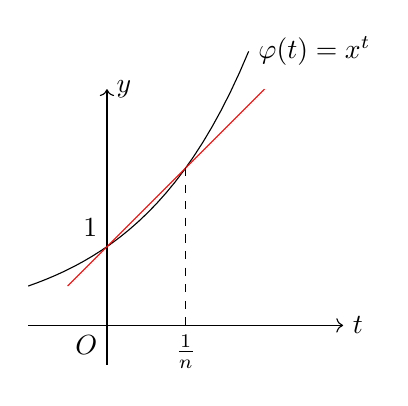
\begin{tikzpicture}
            \draw[->] (-1,0)--(3,0) node [right] {$t$};
            \draw[->] (0,-0.5)--(0,3) node [right] {$y$};
            \node at (0,0) [below left] {$O$};
            \node at (0,1) [above left] {$1$};
            \draw[domain=-1:1.8] plot(\x,{2^\x}) node [right] {$\varphi(t)=x^t$};
            \draw[-,red] (-0.5,0.5)--(2,3);
            \draw[-,dashed] (1,2)--(1,0) node [below] {$\frac{1}{n}$};
        \end{tikzpicture}
    \end{center}

    从而 $f_n(x)$ 单调不降且 $f_n(x)\to -\varphi'(0)=-\ln x=\ln\frac{1}{x}$.

    由 Dini 定理知在任何紧区间 $[a,b]\subset(0,\infty)$ 上有 $f_n\rightrightarrows\ln\frac{1}{x}$.

    但另一方面,若取定义域为 $(0,+\infty)$,则
$$
\Delta_n=\sup_{x\in(0,\infty)}\abs{f(x)-f_n(x)}=+\infty
$$

    从而 $\Delta_n\not\to 0$. 故 $f_n\not\rightrightarrows\ln\frac{1}{x}$.
\end{proof}

\mysubsection{极限与积分运算}

\begin{theorem}
    设 $f_t:[a,b]\to\RR,t\in T$ 是一族函数. 设 $\mathcal{B}_T$ 是 $T$ 的一个基. 若

    \begin{enumerate}
        \item $f_t\underset{\mathcal{B}_T}{\rightrightarrows}f$
        
        \item $\forall t\in T,f_t\in\mathcal{R}[a,b]$
    \end{enumerate}

    则 $f\in\mathcal{R}[a,b]$ 且
$$
\int_a^bf(x)\dd x=\lim_{\mathcal{B}_T}\int_a^bf_t(x)\dd x
$$
\end{theorem}
\begin{proof}
    我们希望使用第 2 节的抽象定理 \ref{sl}. 为此,我们必须找到一个合适的框架:回忆积分是一种特殊的极限,其是关于一个特殊的空间的一个特殊的基取极限.

    定义 $X=\set{(P,\xi)|(P,\xi)\text{ 为 }[a,b]\text{ 带标志点的分划}}$.

    对任意 $\delta>0$ 令 $B_\delta=\set{(P,\xi)\in X|\lambda(P)<\delta}$.
    
    则 $\mathcal{B}_X=\set{B_\delta|\delta>0}$ 构成 $X$ 的一个基.

    考虑一族函数 $F_t:X\to\RR$ 定义为
$$
F_t(P,\xi)\triangleq\sigma(f_t,P,\xi)=\sum_{j=1}^nf_t(\xi_j)\Delta_j
$$

    由 $f_t\underset{\mathcal{B}_T}{\rightrightarrows}f$ 知 $F_t\underset{\mathcal{B}_T}{\rightrightarrows}F$. 其中 $F(P,\xi)\triangleq\sigma(f,P,\xi)$.

    由 $f_t\in\mathcal{R}[a,b]$ 知
$$
\lim_{\mathcal{B}_X}F_t(P,\xi)=\int_a^bf_t(x)\dd x=A_t
$$

    存在. 从而抽象定理的条件满足. 由该定理可得 $\lim\limits_{\mathcal{B}_T}A_t$ 与 $\lim\limits_{\mathcal{B}_X}F(P,\xi)$ 均存在且
$$
\lim_{\mathcal{B}_T}\int_a^bf_t(x)\dd x=\lim_{\mathcal{B}_T}A_t=\lim_{\mathcal{B}_X}F(P,\xi)=\int_a^bf(x)\dd x
$$
\end{proof}

\begin{inference}
    设 $f_n:[a,b]\to\RR$ 满足 $f_n\in\mathcal{R}[a,b]$.

    且 $\sum\limits_{n=1}^\infty f_n(x)$ 在 $[a,b]$ 上一致收敛,则 $\sum\limits_{n=1}^\infty f_n\in\mathcal{R}[a,b]$ 且
$$
\int_a^b\sum\limits_{n=1}^\infty f_n(x)\dd x=\sum_{n=1}^\infty\int_a^b f_n(x)\dd x
$$
\end{inference}

\begin{example}
    在第一卷我们定义过函数
$$
\mathrm{Si}(x)\triangleq\int_0^x\frac{\sin t}{t}\dd t
$$

    现在利用刚证的性质我们可以给出 $\mathrm{Si}(x)$ 的一个幂级数公式. 事实上
$$
\frac{\sin x}{x}=\sum_{n=0}^\infty\frac{(-1)^nx^{2n}}{(2n+1)!}
$$

    由其收敛半径为 $+\infty$ 知该幂级数在任何有界区间上均一致收敛. 从而由推论可知
$$
\begin{aligned}
    \mathrm{Si}(x)&=\int_0^x\frac{\sin t}{t}\dd t=\sum_{n=0}^\infty\frac{(-1)^n}{(2n+1)!}\int_0^xt^{2n}\dd t\\
    &=\sum_{n=0}^\infty\frac{(-1)^nx^{2n+1}}{(2n+1)!(2n+1)}
\end{aligned}
$$

    其收敛半径仍为 $+\infty$.

    特别的,在任何有界区间上,我们可以用多项式来一致逼近 $\mathrm{Si}(x)$.
\end{example}

\mysubsection{极限与微分运算}

接下来,我们讨论可微函数列在取完极限之后保持可微性的条件.

\begin{theorem}
    设 $X\subset\RR^n$ 为有界凸集. 设 $f_t:X\to\RR,t\in T$ 是一族函数. 设 $\mathcal{B}$ 是 $T$ 的一个基.

    若以下三个条件成立

    \begin{enumerate}
        \item $\forall t\in T,f_t$ 均在 $X$ 上可导.
        
        \item $f_t'\underset{\mathcal{B}}{\rightrightarrows}\varphi:X\to\RR$.
        
        \item $\exists x_0\in X,\lim\limits_{\mathcal{B}}f_t(x_0)$ 存在.
    \end{enumerate}

    则 $f_t\underset{\mathcal{B}}{\rightrightarrows}{f}$ 且 $f$ 在 $X$ 上可导,$f'=\varphi$.
\end{theorem}
\begin{proof}
    先证 $f_t\underset{\mathcal{B}}{\rightrightarrows}f$. 为此我们验证 Cauchy 准则:

    任取 $x\in X,t_1,t_2\in T$. 由有限增量定理
$$
\abs{f_{t_1}(x)-f_{t_2}(x)-(f_{t_1}(x_0)-f_{t_2}(x_0))}\le\sup_{\xi\in[x_0,x]}\abs{f_{t_1}'(\xi)-f_{t_2}'(\xi)}\abs{x-x_0}
$$

    由 $f_t'\underset{\mathcal{B}}{\rightrightarrows}\varphi$ 以及 $\lim\limits_{\mathcal{B}}f_t(x_0)$ 存在知
$$
\forall\eps>0,\exists B\in\mathcal{B},\forall t_1,t_2\in B,\forall x\in K,\abs{f_{t_1}'(x)-f_{t_2}'(x)}<\eps,\abs{f_{t_1}(x)-f_{t_2}(x)}<\eps
$$

    从而对 $\forall x\in X$ 有
$$
\abs{f_{t_1}(x)-f_{t_2}(x)}<\eps+\eps d(X)
$$

    由 Cauchy 准则知 $\set{f_t}$ 在 $\mathcal{B}$ 下一致收敛.

    记 $f_t\underset{\mathcal{B}}{\rightrightarrows}f$. 下证 $f$ 在 $X$ 上可微且 $f'=\varphi$.

    为此我们需证:若 $x\in X,x+h\in X$ 有
$$
F(h)\triangleq\frac{\abs{f(x+h)-f(x)-\varphi(x)h}}{\abs{h}}\to 0\quad(h\to 0)
$$

    我们希望使用定理 \ref{sl} 来证明该结论. 为此考虑
$$
F_t(h)\triangleq\frac{\abs{f_t(x+h)-f_t(x)-f_t'(x)h}}{\abs{h}}
$$

    一方面,对于固定的 $t\in T$ 由 $f_t$ 在 $x$ 处可导知
$$
\lim_{h\to 0}F_t(h)=0
$$

    另一方面,我们来验证 $F_t(h)\underset{\mathcal{B}}{\rightrightarrows}F(h)$.

    首先显然有 $F_t(h)\xrightarrow[\mathcal{B}]{}F(h)$.

    从而只需对 $\set{F_t(h):t\in T}$ 验证 Cauchy 准则.

    任取 $t_1,t_2\in T$ 由有限增量定理有
$$
\begin{aligned}
    &\abs{(f_{t_1}(x+h)-f_{t_1}(x)-f_{t_1}'(x)h)-(f_{t_2}(x+h)-f_{t_2}(x)-f_{t_2}'(x)h)}\\
    \le&\sup_{\xi\in[x,x+h]}\abs{(f_{t_1}'(\xi)-f_{t_2}'(\xi))-(f_{t_1}'(x)-f_{t_2}'(x))}\abs{h}
\end{aligned}
$$

    由 $f_t'\underset{\mathcal{B}}{\rightrightarrows}\varphi$ 知
$$
\forall\eps>0,\exists B\in\mathcal{B},\forall t_1,t_2\in B,\forall x\in X,\abs{f_{t_1}'(x)-f_{t_2}'(x)}<\eps
$$

    从而对 $\forall h\ne 0$ 有
$$
\abs{F_{t_1}(h)-F_{t_2}(h)}<\frac{(\eps+\eps)\abs{h}}{\abs{h}}=2\eps
$$

    即 $\set{F_t}$ 在 $\mathcal{B}$ 下一致收敛. 从而 $F_t\underset{\mathcal{B}}{\rightrightarrows}F$.

    现在由定理 \ref{sl} 知 $\lim\limits_{h\to 0}F(h)$ 与 $\lim\limits_{\mathcal{B}}\lim\limits_{h\to 0}F_t(h)$ 均存在且二者相等.

    从而 $\lim\limits_{h\to 0}F(h)=0$. 即 $f$ 在 $x$ 处可导且 $f'(x)=\varphi(x)$.
\end{proof}

\begin{inference}
    设 $X\subset\RR^n$ 为有界凸集. 设 $f_n:X\to\RR$ 在 $X$ 上可微.

    设 $\sum\limits_{n=1}^\infty f_n'(x)$ 在 $X$ 上一致收敛,且 $\exists x_0\in X,\sum\limits_{n=1}^\infty f_n(x_0)$ 收敛.

    则 $\sum\limits_{n=1}^\infty f_n(x)$ 在 $X$ 上一致收敛,极限函数可微且满足
$$
\left(\sum\limits_{n=1}^\infty f_n(x)\right)'=\sum\limits_{n=1}^\infty f_n'(x)
$$
\end{inference}

\mysection{连续函数空间的紧子集与稠密子集}

本节,我们证明两个十分重要的定理. 它们分别刻画了紧空间上的连续函数空间的紧子集与稠密子集.

\mysubsection{Arzelà-Ascoli 定理}

\begin{definition}
    设 $X$ 为集合,$(Y,\rho)$ 为度量空间. 设 $\mathscr{F}=\set{f:X\to Y}$ 为一族函数.

    称 $\mathscr{F}$ 一致有界,若所有 $f\in\mathscr{F}$ 的值域之并在 $Y$ 中有界. 即
$$
V\triangleq\set{f(x)|x\in X,f\in\mathscr{F}}
$$

    在 $Y$ 中有界.

    称 $\mathscr{F}$ 完全有界,若 $V$ 是 $Y$ 中的完全有界集.
\end{definition}

\begin{hint}
    若 $Y=\RR^n$ 或 $\mathbb{C}^n$,则 $A\subset Y$ 有界 $\iff A$ 完全有界.

    从而在此时函数族 $\mathscr{F}$ 一致有界与完全有界等价.

    但若 $Y$ 为无穷维赋范线性空间,则完全有界的概念严格强于有界. 例如 $Y=C[a,b]$.
\end{hint}

\begin{definition}
    设 $(X,d),(Y,\rho)$ 均为度量空间,$\mathscr{F}=\set{f:X\to Y}$ 为一族函数.

    称 $\mathscr{F}$ 等度连续,若
$$
\forall\eps>0,\exists\delta>0,\forall x_1,x_2\in X,d(x_1,x_2)<\delta\implies\forall f\in\mathscr{F},\rho(f(x_1),f(x_2))<\eps
$$
\end{definition}

\begin{example}
    $\mathscr{F}=\set{x^n|n\ge 1},X=[0,1]$.

    则 $\mathscr{F}$ 一致有界,但不等度连续.
\end{example}

\begin{example}
    $\mathscr{F}=\set{\sin nx|n\in\mathbb{N}}$ 在任何区间 $[a,b]$ 上均不等度连续.
\end{example}

\begin{example}
    若 $\mathscr{F}$ 是一族从 $\RR$ 到 $\RR$ 的映射,且
$$
\exists L>0,\forall f\in\mathscr{F},\forall x,y\in\RR,\abs{f(x)-f(y)}\le L\abs{x-y}
$$

    则 $\mathscr{F}$ 等度连续.
\end{example}

如上的概念与一致收敛性有密切的连续:

\begin{lemma}
    设 $K$ 为紧度量空间,$Y$ 为完备度量空间.

    设 $f_n\in C(K;Y)$. 若 $\set{f_n}$ 在 $K$ 上一致收敛,则 $\set{f_n}$ 在 $K$ 上完全有界且等度连续.
\end{lemma}
\begin{proof}
    设 $f_n\rightrightarrows f:K\to Y$. 则 $f$ 也连续.

    \begin{itemize}
        \item 完全有界:
        
        由 $f_n,f$ 连续且 $K$ 紧知 $f_n(K),f(K)$ 均为 $Y$ 中的紧集. 从而完全有界. 由 $f(K)$ 完全有界知
$$
\forall\eps>0,\exists x_1,\cdots,x_k\in K,f(K)\subset\bigcup_{j=1}^kB\left(f(x_j),\frac{\eps}{2}\right)
$$

        由 $f_n\rightrightarrows f$ 知
$$
\begin{aligned}
    \exists N\in\mathbb{N},\forall n\ge N,&\forall x\in K,\abs{f_n(x)-f(x)}<\frac{\eps}{2}\\
    \implies&f_n(K)\subset\bigcup_{j=1}^kB(f(x_j),\eps)
\end{aligned}
$$

        故 $\bigcup\limits_{n\ge N}f_n(K)$ 完全有界.

        由 $f_1(K)\cup\cdots\cup f_N(K)$ 是有限个完全有界集之并,知其完全有界. 故
$$
V\triangleq\bigcup_{n=1}^\infty f_n(K)=\bigcup_{n=1}^Nf_n(K)\cup\bigcup_{n\ge N}f_n(K)
$$

        完全有界. 即 $\set{f_n}$ 完全有界.
        
        \item 等度连续:
        
        任取 $\eps>0$. 由 $f_n\rightrightarrows f$ 知
$$
\exists N\in\mathbb{N},\forall n\ge N,\forall x\in K,\abs{f_n(x)-f(x)}<\frac{\eps}{3}
$$

        由 $f_1,\cdots,f_N,f$ 在紧集 $K$ 上连续知它们一致连续. 从而
$$
\begin{aligned}
    \exists\delta>0,\forall x,x'\in K,d(x,x')<\delta\implies&\rho(f_j(x),f_j(x'))<\frac{\eps}{3},1\le j\le N\\
    &\rho(f(x),f(x'))<\frac{\eps}{3}
\end{aligned}
$$

        则对 $n\ge N$ 有
$$
\begin{aligned}
    \forall x,x'\in K,d(x,x')<\delta\implies&\rho(f_n(x),f_n(x'))\\
    \le&\rho(f_n(x),f(x))+\rho(f(x),f(x'))+\rho(f(x'),f_n(x'))\\
    <&\frac{\eps}{3}+\frac{\eps}{3}+\frac{\eps}{3}=\eps
\end{aligned}
$$

        即 $\set{f_n}$ 等度连续.
    \end{itemize}
\end{proof}

现在我们可以陈述 Arzelà-Ascoli 定理.

\begin{theorem}[Arzelà-Ascoli]
    设 $\mathscr{F}$ 是一族从紧度量空间 $K$ 到完备度量空间 $Y$ 的函数. 则

    $\forall\set{f_n}\subset\mathscr{F}$,存在子列 $n_k$ 使得 $\set{f_{n_k}}$ 一致收敛 $\iff\mathscr{F}$ 完全有界且等度连续.
\end{theorem}
\begin{proof}
    $\implies$:反证,设 $\mathscr{F}$ 不完全有界,即 $V=\set{f(x)|x\in K,f\in\mathscr{F}}$ 不完全有界.
    
    即存在 $\eps_0>0$ 使得 $V$ 不存在有限 $\eps_0$-网.

    则可以构造 $f_n\in\mathscr{F},x_n\in K$ 满足
$$
\rho(f_n(x_n),f_m(x_m))\ge\eps_0,\forall n\ne m
$$

    这说明 $\set{f_n}\subset\mathscr{F}$ 不完全有界,且 $\set{f_n}$ 的任何子列也不完全有界. 从而由引理知其不可能一致收敛.

    反证,设 $\mathscr{F}$ 不等度连续.

    则存在 $\eps_0>0$ 以及 $f_n\in\mathscr{F},x_n,x_n'\in K$ 满足
$$
\begin{cases}
    d(x_n,x_n')<\dfrac{1}{n}\\
    \rho(f_n(x_n),f_n(x_n'))\ge\eps_0
\end{cases},\forall n\in\mathbb{N}
$$

    则 $\set{f_n}$ 的任何子列都不等度连续. 从而不可能一致收敛.

    $\impliedby$:下设 $\mathscr{F}$ 完全有界且等度连续.

    设 $\set{f_n}\subset\mathscr{F}$. 由 $K$ 紧知:存在可数集 $D\subset K$ 使得 $\overline{D}=K$.

    可以这样构造:$\forall n\in\mathbb{N}$ 存在 $K$ 的有限 $\dfrac{1}{n}$-网 $D_n$. 令 $D=\bigcup\limits_{n\in\mathbb{N}}D_n$ 即可.

    现在对 $\set{f_n}$ 利用 Cantor 对角线法,可以选出子列 $\set{f_{n_k}}$ 使得 $\forall x\in D$ 有 $f_{n_k}(x)\to f_\infty(x),k\to\infty$.

    这里能选出子列的原因是 $\forall x\in D,\set{f_n(x)}$ 完全有界且 $Y$ 完备.

    下证:$\set{f_{n_k}}$ 一致收敛.

    任取 $\eps>0$. 由 $\mathscr{F}$ 等度连续知
$$
\exists\delta>0,\forall f\in\mathscr{F},\forall x,x'\in K,d(x,x')<\delta\implies\rho(f(x),f(x'))<\frac{\eps}{4}
$$

    由 $D\subset K$ 知 $D$ 完全有界. 从而其存在有限 $\dfrac{\delta}{2}$-网,记为 $\set{x_1,\cdots,x_m}\subset D$.

    由 $f_{n_k}(x_i)\to f_\infty(x_i),i=1,\cdots,m$ 知
$$
\exists K\in\mathbb{N},\forall k\ge K,\forall 1\le i\le m,\rho(f_{n_k}(x_i),f_\infty(x_i))<\frac{\eps}{4}
$$

    现任取 $k,l\ge K$. 则对 $\forall x\in K$ 可以选出 $x_i$ 使得 $d(x,x_i)<\delta$. 从而
$$
\begin{aligned}
    \rho(f_{n_k}(x),f_{n_l}(x))\le&\rho(f_{n_k}(x),f_{n_k}(x_i))+\rho(f_{n_k}(x_i),f_\infty(x_i))\\
    &+\rho(f_\infty(x_i),f_{n_l}(x_i))+\rho(f_{n_l}(x_i),f_{n_l}(x))\\
    <&\frac{\eps}{4}+\frac{\eps}{4}+\frac{\eps}{4}+\frac{\eps}{4}=\eps
\end{aligned}
$$

    即 $\set{f_{n_k}}$ 满足 Cauchy 准则,从而一致收敛.
\end{proof}

\end{document}